% Contents from body/native-chapter.tex.
% Chapter I opening, fixed to the original printed pages 1--14.
\pagenumbering{arabic}
\begingroup
\renewenvironment{problems}
  {\begin{description}[style=multiline,labelwidth=2.6em,labelsep=.35em,leftmargin=2.95em,itemsep=3.4pt,parsep=1pt,topsep=2pt]}
  {\end{description}}
\renewcommand{\Problem}[3][]{%
  \item[{\normalfont\bfseries\llap{#1}\Num{x#2}{#2}.}]\ignorespaces#3}
\renewcommand{\Figure}[4]{%
  \par\medskip
  {\centering\noindent\resizebox{#3\linewidth}{!}{\input{figures/#2.tex}}\par
  \smallskip\small\textbf{Figure \Num{fig#1}{#1}.}\quad #4\par}
  \medskip}
\newcommand{\OriginalSectionHeading}[2]{%
  \par\addvspace{14pt}\noindent
  \refstepcounter{section}%
  \textbf{\large\Num{#1}{\thesection}\quad #2}\par\smallskip\noindent}
\BookMark{0}{I  Varieties}{p-15}
\BookMark{1}{1.1  Affine Varieties}{sec-I-1}
\BeginTypeSheet{15}{1}{}{1}
\Opening{53}{577}{p-15}{I}{Varieties}
\put(53,399){\makebox(0,0)[lt]{\parbox[t]{333.37bp}{%
\normalfont\fontsize{10}{11.5}\selectfont
\setlength{\parindent}{11pt}%
\setlength{\parskip}{1.15pt}%
\noindent\refstepcounter{chapter}%
Our purpose in this chapter is to give an introduction to algebraic geometry with as little machinery as possible. We work over a fixed algebraically closed field $k$. We define the main objects of study, which are algebraic varieties in affine or projective space. We introduce some of the most important concepts, such as dimension, regular functions, rational maps, nonsingular varieties, and the degree of a projective variety. And most important, we give lots of specific examples, in the form of exercises at the end of each section. The examples have been selected to illustrate many interesting and important phenomena, beyond those mentioned in the text. The person who studies these examples carefully will not only have a good understanding of the basic concepts of algebraic geometry, but he will also have the background to appreciate some of the more abstract developments of modern algebraic geometry, and he will have a resource against which to check his intuition. We will continually refer back to this library of examples in the rest of the book.

The last section of this chapter is a kind of second introduction to the book. It contains a discussion of the \textquotedblleft{}classification problem,\textquotedblright{} which has motivated much of the development of algebraic geometry. It also contains a discussion of the degree of generality in which one should develop the foundations of algebraic geometry, and as such provides motivation for the theory of schemes.

\OriginalSectionHeading{s1}{Affine Varieties}
Let $k$ be a fixed algebraically closed field. We define \emph{affine $n$-space over $k$}, denoted $\AffSpace[k]{n}$ or simply $\AffSpace{n}$, to be the set of all $n$-tuples of elements of $k$. An element $P\in\AffSpace{n}$ will be called a \emph{point}, and if $P=(a_1,\ldots,a_n)$ with $a_i\in k$, then the $a_i$ will be called the \emph{coordinates} of $P$.
\par}}}
\EndSheet
\ChapterSheet{16}{2}{\Goto{p-15}{I\quad Varieties}}{%
\indent Let $A=k[x_1,\ldots,x_n]$ be the polynomial ring in $n$ variables over $k$. We will interpret the elements of $A$ as functions from the affine $n$-space to $k$, by defining $f(P)=f(a_1,\ldots,a_n)$, where $f\in A$ and $P\in\AffSpace{n}$. Thus if $f\in A$ is a polynomial, we can talk about the set of \emph{zeros} of $f$, namely $Z(f)=\{P\in\AffSpace{n}\mid f(P)=0\}$. More generally, if $T$ is any subset of $A$, we define the \emph{zero set} of $T$ to be the common zeros of all the elements of $T$, namely
\[
Z(T)=\{P\in\AffSpace{n}\mid f(P)=0\text{ for all }f\in T\}.
\]
Clearly if $\ideal$ is the ideal of $A$ generated by $T$, then $Z(T)=Z(\ideal)$. Furthermore, since $A$ is a noetherian ring, any ideal $\ideal$ has a finite set of generators $f_1,\ldots,f_r$. Thus $Z(T)$ can be expressed as the common zeros of the finite set of polynomials $f_1,\ldots,f_r$.

\Dfn A subset $Y$ of $\AffSpace{n}$ is an \emph{algebraic set} if there exists a subset $T\subseteq A$ such that $Y=Z(T)$.

\begin{result}{Proposition}{1.1}{r1.1}
The union of two algebraic sets is an algebraic set. The intersection of any family of algebraic sets is an algebraic set. The empty set and the whole space are algebraic sets.
\end{result}
\Proof If $Y_1=Z(T_1)$ and $Y_2=Z(T_2)$, then $Y_1\cup Y_2=Z(T_1T_2)$, where $T_1T_2$ denotes the set of all products of an element of $T_1$ by an element of $T_2$. Indeed, if $P\in Y_1\cup Y_2$, then either $P\in Y_1$ or $P\in Y_2$, so $P$ is a zero of every polynomial in $T_1T_2$. Conversely, if $P\in Z(T_1T_2)$, and $P\notin Y_1$ say, then there is an $f\in T_1$ such that $f(P)\ne 0$. Now for any $g\in T_2$, $(fg)(P)=0$ implies that $g(P)=0$, so that $P\in Y_2$.

If $Y_\alpha=Z(T_\alpha)$ is any family of algebraic sets, then $\bigcap Y_\alpha=Z(\bigcup T_\alpha)$, so $\bigcap Y_\alpha$ is also an algebraic set. Finally, the empty set $\varnothing=Z(1)$, and the whole space $\AffSpace{n}=Z(0)$.

\Dfn We define the \emph{Zariski topology} on $\AffSpace{n}$ by taking the open subsets to be the complements of the algebraic sets. This is a topology, because according to the proposition, the intersection of two open sets is open, and the union of any family of open sets is open. Furthermore, the empty set and the whole space are both open.

\Observation{Example}{1.1.1}{r1.1.1} Let us consider the Zariski topology on the affine line $\AffSpace{1}$. Every ideal in $A=k[x]$ is principal, so every algebraic set is the set of zeros of a single polynomial. Since $k$ is algebraically closed, every nonzero polynomial $f(x)$ can be written $f(x)=c(x-a_1)\cdots(x-a_n)$ with $c,a_1,\ldots,a_n\in k$. Then $Z(f)=\{a_1,\ldots,a_n\}$. Thus the algebraic sets in $\AffSpace{1}$ are just the finite subsets (including the empty set) and the whole space (corresponding to $f=0$). Thus the open sets are the empty set and the complements of finite subsets. Notice in particular that this topology is not Hausdorff.
}

\ChapterSheet{17}{3}{\Goto{sec-I-1}{1\quad Affine Varieties}}{%
\Dfn A nonempty subset $Y$ of a topological space $X$ is \emph{irreducible} if it cannot be expressed as the union $Y=Y_1\cup Y_2$ of two proper subsets, each one of which is closed in $Y$. The empty set is not considered to be irreducible.

\Observation{Example}{1.1.2}{r1.1.2} $\AffSpace{1}$ is irreducible, because its only proper closed subsets are finite, yet it is infinite (because $k$ is algebraically closed, hence infinite).

\Observation{Example}{1.1.3}{r1.1.3} Any nonempty open subset of an irreducible space is irreducible and dense.

\Observation{Example}{1.1.4}{r1.1.4} If $Y$ is an irreducible subset of $X$, then its closure $\overline Y$ in $X$ is also irreducible.

\Dfn An \emph{affine algebraic variety} (or simply \emph{affine variety}) is an irreducible closed subset of $\AffSpace{n}$ (with the induced topology). \hypertarget{err-I-quasiaffine}{}\EditionText{A nonempty open subset of an affine variety} is a \emph{quasi-affine variety}.

These affine and quasi-affine varieties are our first objects of study. But before we can go further, in fact before we can even give any interesting examples, we need to explore the relationship between subsets of $\AffSpace{n}$ and ideals in $A$ more deeply. So for any subset $Y\subseteq\AffSpace{n}$, let us define the \emph{ideal} of $Y$ in $A$ by
\[
I(Y)=\{f\in A\mid f(P)=0\text{ for all }P\in Y\}.
\]
Now we have a function $Z$ which maps subsets of $A$ to algebraic sets, and a function $I$ which maps subsets of $\AffSpace{n}$ to ideals. Their properties are summarized in the following proposition.

\begin{result}{Proposition}{1.2}{r1.2}
\begin{parts}
\Part{r1.2a}{a} If $T_1\subseteq T_2$ are subsets of $A$, then $Z(T_1)\supseteq Z(T_2)$.
\Part{r1.2b}{b} If $Y_1\subseteq Y_2$ are subsets of $\AffSpace{n}$, then $I(Y_1)\supseteq I(Y_2)$.
\Part{r1.2c}{c} For any two subsets $Y_1,Y_2$ of $\AffSpace{n}$, we have $I(Y_1\cup Y_2)=I(Y_1)\cap I(Y_2)$.
\Part{r1.2d}{d} For any ideal $\ideal\subseteq A$, $I(Z(\ideal))=\sqrt{\ideal}$, the radical of $\ideal$.
\Part{r1.2e}{e} For any subset $Y\subseteq\AffSpace{n}$, $Z(I(Y))=\overline Y$, the closure of $Y$.
\end{parts}
\end{result}
\Proof \BookLink{r1.2a}{(a)}, \BookLink{r1.2b}{(b)} and \BookLink{r1.2c}{(c)} are obvious. \BookLink{r1.2d}{(d)} is a direct consequence of Hilbert's Nullstellensatz, stated below, since the radical of $\ideal$ is defined as
\[
\sqrt{\ideal}=\{f\in A\mid f^r\in\ideal\text{ for some }r>0\}.
\]
To prove \BookLink{r1.2e}{(e)}, we note that $Y\subseteq Z(I(Y))$, which is a closed set, so clearly $\overline Y\subseteq Z(I(Y))$. On the other hand, let $W$ be any closed set containing $Y$. Then $W=Z(\ideal)$ for some ideal $\ideal$. So $Z(\ideal)\supseteq Y$, and by \BookLink{r1.2b}{(b)}, $IZ(\ideal)\subseteq I(Y)$. But certainly $\ideal\subseteq IZ(\ideal)$, so by \BookLink{r1.2a}{(a)} we have $W=Z(\ideal)\supseteq ZI(Y)$. Thus $ZI(Y)=\overline Y$.
}

\ChapterSheet{18}{4}{\Goto{p-15}{I\quad Varieties}}{%
\begin{namedresult}{Theorem}{1.3A}{r1.3A}{Hilbert's Nullstellensatz}
Let $k$ be an algebraically closed field, let $\ideal$ be an ideal in $A=k[x_1,\ldots,x_n]$, and let $f\in A$ be a polynomial which vanishes at all points of $Z(\ideal)$. Then $f^r\in\ideal$ for some integer $r>0$.
\end{namedresult}
\Proof Lang \BookLink{b-lang}{[2, p.~256]} or Atiyah--Macdonald \BookLink{b-am}{[1, p.~85]} or Zariski--Samuel \BookLink{b-zs}{[1, vol.~2, p.~164]}.

\begin{result}{Corollary}{1.4}{r1.4}
There is a one-to-one inclusion-reversing correspondence between algebraic sets in $\AffSpace{n}$ and radical ideals (i.e., ideals which are equal to their own radical) in $A$, given by $Y\mapsto I(Y)$ and $\ideal\mapsto Z(\ideal)$. Furthermore, an algebraic set is irreducible if and only if its ideal is a prime ideal.
\end{result}
\Proof Only the last part is new. If $Y$ is irreducible, we show that $I(Y)$ is prime. Indeed, if $fg\in I(Y)$, then $Y\subseteq Z(fg)=Z(f)\cup Z(g)$. Thus $Y=(Y\cap Z(f))\cup(Y\cap Z(g))$, both being closed subsets of $Y$. Since $Y$ is irreducible, we have either $Y=Y\cap Z(f)$, in which case $Y\subseteq Z(f)$, or $Y\subseteq Z(g)$. Hence either $f\in I(Y)$ or $g\in I(Y)$.

Conversely, let $\mathfrak p$ be a prime ideal, and suppose that $Z(\mathfrak p)=Y_1\cup Y_2$. Then $\mathfrak p=I(Y_1)\cap I(Y_2)$, so either $\mathfrak p=I(Y_1)$ or $\mathfrak p=I(Y_2)$. Thus $Z(\mathfrak p)=Y_1$ or $Y_2$, hence it is irreducible.

\Observation{Example}{1.4.1}{r1.4.1} $\AffSpace{n}$ is irreducible, since it corresponds to the zero ideal in $A$, which is prime.

\Observation{Example}{1.4.2}{r1.4.2} Let $f$ be an irreducible polynomial in $A=k[x,y]$. Then $f$ generates a prime ideal in $A$, since $A$ is a unique factorization domain, so the zero set $Y=Z(f)$ is irreducible. We call it the \emph{affine curve} defined by the equation $f(x,y)=0$. If $f$ has degree $d$, we say that $Y$ is a curve of \emph{degree} $d$.

\Observation{Example}{1.4.3}{r1.4.3} More generally, if $f$ is an irreducible polynomial in $A=k[x_1,\ldots,x_n]$, we obtain an affine variety $Y=Z(f)$, which is called a \emph{surface} if $n=3$, or a \emph{hypersurface} if $n>3$.

\Observation{Example}{1.4.4}{r1.4.4} A maximal ideal $\mathfrak m$ of $A=k[x_1,\ldots,x_n]$ corresponds to a minimal irreducible closed subset of $\AffSpace{n}$, which must be a point, say $P=(a_1,\ldots,a_n)$. This shows that every maximal ideal of $A$ is of the form $\mathfrak m=(x_1-a_1,\ldots,x_n-a_n)$, for some $a_1,\ldots,a_n\in k$.

\Observation{Example}{1.4.5}{r1.4.5} If $k$ is not algebraically closed, these results do not hold. For example, if $k=\RR$, the curve $x^2+y^2+1=0$ in $\AffSpace[\RR]{2}$ has no points. So \BookLink{r1.2d}{(1.2d)} is false. See also (Ex.~\BookLink{x1.12}{1.12}).

\Dfn If $Y\subseteq\AffSpace{n}$ is an affine algebraic set, we define the \emph{affine coordinate ring} $A(Y)$ of $Y$, to be $A/I(Y)$.

\Observation{Remark}{1.4.6}{r1.4.6} If $Y$ is an affine variety, then $A(Y)$ is an integral domain. Furthermore, $A(Y)$ is a finitely generated $k$-algebra. Conversely, any
}

\ChapterSheet{19}{5}{\Goto{sec-I-1}{1\quad Affine Varieties}}{%
finitely generated $k$-algebra $B$ which is a domain is the affine coordinate ring of some affine variety. Indeed, write $B$ as the quotient of a polynomial ring $A=k[x_1,\ldots,x_n]$ by an ideal $\ideal$, and let $Y=Z(\ideal)$.

Next we will study the topology of our varieties. To do so we introduce an important class of topological spaces which includes all varieties.

\Dfn A topological space $X$ is called \emph{noetherian} if it satisfies the \emph{descending chain condition} for closed subsets: for any sequence $Y_1\supseteq Y_2\supseteq\cdots$ of closed subsets, there is an integer $r$ such that $Y_r=Y_{r+1}=\cdots$.

\Observation{Example}{1.4.7}{r1.4.7} $\AffSpace{n}$ is a noetherian topological space. Indeed, if $Y_1\supseteq Y_2\supseteq\cdots$ is a descending chain of closed subsets, then $I(Y_1)\subseteq I(Y_2)\subseteq\cdots$ is an ascending chain of ideals in $A=k[x_1,\ldots,x_n]$. Since $A$ is a noetherian ring, this chain of ideals is eventually stationary. But for each $i$, $Y_i=Z(I(Y_i))$, so the chain $Y_i$ is also stationary.

\begin{result}{Proposition}{1.5}{r1.5}
In a noetherian topological space $X$, every nonempty closed subset $Y$ can be expressed as a finite union $Y=Y_1\cup\cdots\cup Y_r$ of irreducible closed subsets $Y_i$. If we require that $Y_i\not\supseteq Y_j$ for $i\ne j$, then the $Y_i$ are uniquely determined. They are called the \textup{irreducible components} of $Y$.
\end{result}
\Proof First we show the existence of such a representation of $Y$. Let $\mathfrak S$ be the set of nonempty closed subsets of $X$ which \emph{cannot} be written as a finite union of irreducible closed subsets. If $\mathfrak S$ is nonempty, then since $X$ is noetherian, it must contain a minimal element, say $Y$. Then $Y$ is not irreducible, by construction of $\mathfrak S$. Thus we can write $Y=Y'\cup Y''$, where $Y'$ and $Y''$ are proper closed subsets of $Y$. By minimality of $Y$, each of $Y'$ and $Y''$ can be expressed as a finite union of closed irreducible subsets, hence $Y$ also, which is a contradiction. We conclude that every closed set $Y$ can be written as a union $Y=Y_1\cup\cdots\cup Y_r$ of irreducible subsets. By throwing away a few if necessary, we may assume $Y_i\not\supseteq Y_j$ for $i\ne j$.

Now suppose $Y=Y'_1\cup\cdots\cup Y'_s$ is another such representation. Then $Y'_1\subseteq Y=Y_1\cup\cdots\cup Y_r$, so $Y'_1=\bigcup(Y'_1\cap Y_i)$. But $Y'_1$ is irreducible, so $Y'_1\subseteq Y_i$ for some $i$, say $i=1$. Similarly, $Y_1\subseteq Y'_j$ for some $j$. Then $Y'_1\subseteq Y'_j$, so $j=1$, and we find that $Y_1=Y'_1$. Now let $Z=\overline{(Y-Y_1)}$. Then $Z=Y_2\cup\cdots\cup Y_r$ and also $Z=Y'_2\cup\cdots\cup Y'_s$. So proceeding by induction on $r$, we obtain the uniqueness of the $Y_i$.

\begin{result}{Corollary}{1.6}{r1.6}
Every algebraic set in $\AffSpace{n}$ can be expressed uniquely as a union of varieties, no one containing another.
\end{result}

\Dfn If $X$ is a topological space, we define the \emph{dimension} of $X$ (denoted $\dim X$) to be the supremum of all integers $n$ such that there exists a chain $Z_0\subset Z_1\subset\cdots\subset Z_n$ of distinct irreducible closed subsets of $X$. We define the \emph{dimension} of an affine or quasi-affine variety to be its dimension as a topological space.
}

\ChapterSheet{20}{6}{\Goto{p-15}{I\quad Varieties}}{%
\Observation{Example}{1.6.1}{r1.6.1} The dimension of $\AffSpace{1}$ is $1$. Indeed, the only irreducible closed subsets of $\AffSpace{1}$ are the whole space and single points.

\Dfn In a ring $A$, the \emph{height} of a prime ideal $\mathfrak p$ is the supremum of all integers $n$ such that there exists a chain $\mathfrak p_0\subset\mathfrak p_1\subset\cdots\subset\mathfrak p_n=\mathfrak p$ of distinct prime ideals. We define the \emph{dimension} (or \emph{Krull dimension}) of $A$ to be the supremum of the heights of all prime ideals.

\begin{result}{Proposition}{1.7}{r1.7}
If $Y$ is an affine algebraic set, then the dimension of $Y$ is equal to the dimension of its affine coordinate ring $A(Y)$.
\end{result}
\Proof If $Y$ is an affine algebraic set in $\AffSpace{n}$, then the closed irreducible subsets of $Y$ correspond to prime ideals of $A=k[x_1,\ldots,x_n]$ containing $I(Y)$. These in turn correspond to prime ideals of $A(Y)$. Hence $\dim Y$ is the length of the longest chain of prime ideals in $A(Y)$, which is its dimension.

This proposition allows us to apply results from the dimension theory of noetherian rings to algebraic geometry.

\begin{result}{Theorem}{1.8A}{r1.8A}
Let $k$ be a field, and let $B$ be an integral domain which is a finitely generated $k$-algebra. Then:
\begin{parts}
\Part{r1.8Aa}{a} the dimension of $B$ is equal to the transcendence degree of the quotient field $K(B)$ of $B$ over $k$;
\Part{r1.8Ab}{b} For any prime ideal $\mathfrak p$ in $B$, we have
\[
\textup{height }\mathfrak p+\dim B/\mathfrak p=\dim B.
\]
\end{parts}
\end{result}
\Proof Matsumura \BookLink{b-mat}{[2, Ch.~5, \S14]} or, in the case $k$ is algebraically closed, Atiyah--Macdonald \BookLink{b-am}{[1, Ch.~11]}

\begin{result}{Proposition}{1.9}{r1.9}
The dimension of $\AffSpace{n}$ is $n$.
\end{result}
\Proof According to \BookLink{r1.7}{(1.7)} this says that the dimension of the polynomial ring $k[x_1,\ldots,x_n]$ is $n$, which follows from part \BookLink{r1.8Aa}{(a)} of the theorem.

\begin{result}{Proposition}{1.10}{r1.10}
If $Y$ is a quasi-affine variety, then $\dim Y=\dim\overline Y$.
\end{result}
\Proof If $Z_0\subset Z_1\subset\cdots\subset Z_n$ is a sequence of distinct closed irreducible subsets of $Y$, then $\overline{Z}_0\subset\overline{Z}_1\subset\cdots\subset\overline{Z}_n$ is a sequence of distinct closed irreducible subsets of $\overline Y$ \BookLink{r1.1.4}{(1.1.4)}, so we have $\dim Y\leqslant\dim\overline Y$. In particular, $\dim Y$ is finite, so we can choose a maximal such chain $Z_0\subset\cdots\subset Z_n$, with $n=\dim Y$. In that case $Z_0$ must be a point $P$, and the chain $P=\overline{Z}_0\subset\cdots\subset\overline{Z}_n$ will also be maximal \BookLink{r1.1.3}{(1.1.3)}. Now $P$ corresponds to a maximal ideal $\mathfrak m$ of the affine coordinate ring $A(\overline Y)$ of $\overline Y$. The $\overline{Z}_i$ correspond to prime ideals contained in $\mathfrak m$, so $\textup{height }\mathfrak m=n$. On the other hand, since $P$ is a point in affine space, $A(\overline Y)/\mathfrak m\cong k$ \BookLink{r1.4.4}{(1.4.4)}. Hence by \BookLink{r1.8Ab}{(1.8Ab)} we find that $n=\dim A(\overline Y)=\dim\overline Y$. Thus $\dim Y=\dim\overline Y$.
}

\ChapterSheet{21}{7}{\Goto{sec-I-1}{1\quad Affine Varieties}}{%
\begin{namedresult}{Theorem}{1.11A}{r1.11A}{Krull's Hauptidealsatz}
Let $A$ be a noetherian ring, and let $f\in A$ be an element which is neither a zero divisor nor a unit. Then every minimal prime ideal $\mathfrak p$ containing $f$ has height $1$.
\end{namedresult}
\Proof Atiyah--Macdonald \BookLink{b-am}{[1, p.~122]}.

\begin{result}{Proposition}{1.12A}{r1.12A}
A noetherian integral domain $A$ is a unique factorization domain if and only if every prime ideal of height $1$ is principal.
\end{result}
\Proof Matsumura \BookLink{b-mat}{[2, p.~141]}, or Bourbaki \BookLink{b-bour}{[1, Ch.~7, \S3]}.

\begin{result}{Proposition}{1.13}{r1.13}
A variety $Y$ in $\AffSpace{n}$ has dimension $n-1$ if and only if it is the zero set $Z(f)$ of a single nonconstant irreducible polynomial in $A=k[x_1,\ldots,x_n]$.
\end{result}
\Proof If $f$ is an irreducible polynomial, we have already seen that $Z(f)$ is a variety. Its ideal is the prime ideal $\mathfrak p=(f)$. By \BookLink{r1.11A}{(1.11A)}, $\mathfrak p$ has height $1$, so by \BookLink{r1.8A}{(1.8A)}, $Z(f)$ has dimension $n-1$. Conversely, a variety of dimension $n-1$ corresponds to a prime ideal $\mathfrak p$ of height $1$. Now the polynomial ring $A$ is a unique factorization domain, so by \BookLink{r1.12A}{(1.12A)}, $\mathfrak p$ is principal, necessarily generated by an irreducible polynomial $f$. Hence $Y=Z(f)$.

\Observation{Remark}{1.13.1}{r1.13.1} A prime ideal of height $2$ in a polynomial ring cannot necessarily be generated by two elements (Ex.~\BookLink{x1.11}{1.11}).

{\small\Exercises
\begin{problems}
\Problem{1.1}{\begin{parts}
\Part{x1.1a}{a} Let $Y$ be the plane curve $y=x^2$ (i.e., $Y$ is the zero set of the polynomial $f=y-x^2$). Show that $A(Y)$ is isomorphic to a polynomial ring in one variable over $k$.
\Part{x1.1b}{b} Let $Z$ be the plane curve $xy=1$. Show that $A(Z)$ is not isomorphic to a polynomial ring in one variable over $k$.
\item[{*\Num{x1.1c}{(c)}}] Let $f$ be any irreducible quadratic polynomial in $k[x,y]$, and let $W$ be the conic defined by $f$. Show that $A(W)$ is isomorphic to $A(Y)$ or $A(Z)$. Which one is it when?
\end{parts}}
\Problem{1.2}{\emph{The Twisted Cubic Curve.} Let $Y\subseteq\AffSpace{3}$ be the set $Y=\{(t,t^2,t^3)\mid t\in k\}$. Show that $Y$ is an affine variety of dimension $1$. Find generators for the ideal $I(Y)$. Show that $A(Y)$ is isomorphic to a polynomial ring in one variable over $k$. We say that $Y$ is given by the \emph{parametric representation} $x=t$, $y=t^2$, $z=t^3$.}
\Problem{1.3}{Let $Y$ be the algebraic set in $\AffSpace{3}$ defined by the two polynomials $x^2-yz$ and $xz-x$. Show that $Y$ is a union of three irreducible components. Describe them and find their prime ideals.}
\Problem{1.4}{If we identify $\AffSpace{2}$ with $\AffSpace{1}\times\AffSpace{1}$ in the natural way, show that the Zariski topology on $\AffSpace{2}$ is not the product topology of the Zariski topologies on the two copies of $\AffSpace{1}$.}
\end{problems}}
}

\BookMark{1}{1.2  Projective Varieties}{sec-I-2}
\ChapterSheet{22}{8}{\Goto{p-15}{I\quad Varieties}}{%
{\small\begin{problems}
\Problem{1.5}{Show that a $k$-algebra $B$ is isomorphic to the affine coordinate ring of some algebraic set in $\AffSpace{n}$, for some $n$, if and only if $B$ is a finitely generated $k$-algebra with no nilpotent elements.}
\Problem{1.6}{Any nonempty open subset of an irreducible topological space is dense and irreducible. If $Y$ is a subset of a topological space $X$, which is irreducible in its induced topology, then the closure $\overline Y$ is also irreducible.}
\Problem{1.7}{\begin{parts}
\Part{x1.7a}{a} Show that the following conditions are equivalent for a topological space $X$: \Num{x1.7ai}{(i)} $X$ is noetherian; \Num{x1.7aii}{(ii)} every nonempty family of closed subsets has a minimal element; \Num{x1.7aiii}{(iii)} $X$ satisfies the ascending chain condition for open subsets; \Num{x1.7aiv}{(iv)} every nonempty family of open subsets has a maximal element.
\Part{x1.7b}{b} A noetherian topological space is \emph{quasi-compact}, i.e., every open cover has a finite subcover.
\Part{x1.7c}{c} Any subset of a noetherian topological space is noetherian in its induced topology.
\Part{x1.7d}{d} A noetherian space which is also Hausdorff must be a finite set with the discrete topology.
\end{parts}}
\Problem{1.8}{Let $Y$ be an affine variety of dimension $r$ in $\AffSpace{n}$. Let $H$ be a hypersurface in $\AffSpace{n}$, and assume that $Y\not\subseteq H$. Then every irreducible component of $Y\cap H$ has dimension $r-1$. (See \BookLink{r7.1}{(7.1)} for a generalization.)}
\Problem{1.9}{Let $\ideal\subseteq A=k[x_1,\ldots,x_n]$ be an ideal which can be generated by $r$ elements. Then every irreducible component of $Z(\ideal)$ has dimension $\geqslant n-r$.}
\Problem{1.10}{\begin{parts}
\Part{x1.10a}{a} If $Y$ is any subset of a topological space $X$, then $\dim Y\leqslant\dim X$.
\Part{x1.10b}{b} If $X$ is a topological space which is covered by a family of open subsets $\{U_i\}$, then $\dim X=\sup\dim U_i$.
\Part{x1.10c}{c} Give an example of a topological space $X$ and a dense open subset $U$ with $\dim U<\dim X$.
\Part{x1.10d}{d} If $Y$ is a closed subset of an irreducible finite-dimensional topological space $X$, and if $\dim Y=\dim X$, then $Y=X$.
\Part{x1.10e}{e} Give an example of a noetherian topological space of infinite dimension.
\end{parts}}
\Problem[*]{1.11}{Let $Y\subseteq\AffSpace{3}$ be the curve given parametrically by $x=t^3$, $y=t^4$, $z=t^5$. Show that $I(Y)$ is a prime ideal of height $2$ in $k[x,y,z]$ \hypertarget{err-I-1-11}{}\EditionText{which cannot be generated by $2$ elements even after localization at the origin.} We say $Y$ is \emph{not a local complete intersection}---cf.~(Ex.~\BookLink{x2.17}{2.17}).}
\Problem{1.12}{Give an example of an irreducible polynomial $f\in\RR[x,y]$, whose zero set $Z(f)$ in $\AffSpace[\RR]{2}$ is not irreducible (cf.~\BookLink{r1.4.2}{1.4.2}).}
\end{problems}

}
\OriginalSectionHeading{s2}{Projective Varieties}
To define projective varieties, we proceed in a manner analogous to the definition of affine varieties, except that we work in projective space.

Let $k$ be our fixed algebraically closed field. We \hypertarget{err-1}{}defined \emph{projective $n$-space over $k$}, denoted $\Proj^n_k$, or simply $\Proj^n$, to be the set of equivalence classes of $(n+1)$-tuples $(a_0,\ldots,a_n)$ of elements of $k$, not all zero, under the equivalence relation given by $(a_0,\ldots,a_n)\sim(\lambda a_0,\ldots,\lambda a_n)$ for all $\lambda\in k$, $\lambda\ne 0$. Another way of saying this is that $\Proj^n$ as a set is the quotient of the set
}

\ChapterSheet{23}{9}{\Goto{sec-I-2}{2\quad Projective Varieties}}{%
$\AffSpace{n+1}-\{(0,\ldots,0)\}$ under the equivalence relation which identifies points lying on the same line through the origin.

An element of $\Proj^n$ is called a \emph{point}. If $P$ is a point, then any $(n+1)$-tuple $(a_0,\ldots,a_n)$ in the equivalence class $P$ is called a \emph{set of homogeneous coordinates} for $P$.

Let $S$ be the polynomial ring $k[x_0,\ldots,x_n]$. We want to regard $S$ as a graded ring, so we recall briefly the notion of a graded ring.

A \emph{graded ring} is a ring $S$, together with a decomposition $S=\bigoplus_{d\geqslant0}S_d$ of $S$ into a direct sum of abelian groups $S_d$, such that for any $d,e\geqslant0$, $S_d\cdot S_e\subseteq S_{d+e}$. An element of $S_d$ is called a \emph{homogeneous element of degree $d$}. Thus any element of $S$ can be written uniquely as a (finite) sum of homogeneous elements. An ideal $\ideal\subseteq S$ is a \emph{homogeneous ideal} if $\ideal=\bigoplus_{d\geqslant0}(\ideal\cap S_d)$. We will need a few basic facts about homogeneous ideals (see, for example, Matsumura \BookLink{b-mat}{[2, \S10]} or Zariski--Samuel \BookLink{b-zs}{[1, vol.~2, Ch.~VII, \S2]}). An ideal is homogeneous if and only if it can be generated by homogeneous elements. The sum, product, intersection, and radical of homogeneous ideals are homogeneous. To test whether a \hypertarget{err-2}{}\EditionText{proper homogeneous} ideal is prime, it is sufficient to show for any two \emph{homogeneous} elements $f,g$, that $fg\in\ideal$ implies $f\in\ideal$ or $g\in\ideal$.

We make the polynomial ring $S=k[x_0,\ldots,x_n]$ into a graded ring by taking $S_d$ to be the set of all linear combinations of monomials of total weight $d$ in $x_0,\ldots,x_n$. If $f\in S$ is a polynomial, we cannot use it to define a function on $\Proj^n$, because of the nonuniqueness of the homogeneous coordinates. However, if $f$ is a homogeneous polynomial of degree $d$, then $f(\lambda a_0,\ldots,\lambda a_n)=\lambda^d f(a_0,\ldots,a_n)$, so that the property of $f$ being zero or not depends only on the equivalence class of $(a_0,\ldots,a_n)$. Thus $f$ gives a function from $\Proj^n$ to $\{0,1\}$ by $f(P)=0$ if $f(a_0,\ldots,a_n)=0$, and $f(P)=1$ if $f(a_0,\ldots,a_n)\ne0$.

Thus we can talk about the \emph{zeros} of a homogeneous polynomial, namely $Z(f)=\{P\in\Proj^n\mid f(P)=0\}$. If $T$ is any set of homogeneous elements of $S$, we define the \emph{zero set} of $T$ to be
\[
Z(T)=\{P\in\Proj^n\mid f(P)=0\text{ for all } f\in T\}.
\]
If $\ideal$ is a homogeneous ideal of $S$, we define $Z(\ideal)=Z(T)$, where $T$ is the set of all homogeneous elements in $\ideal$. Since $S$ is a noetherian ring, any set of homogeneous elements $T$ has a finite subset $f_1,\ldots,f_r$ such that $Z(T)=Z(f_1,\ldots,f_r)$.

\Dfn A subset $Y$ of $\Proj^n$ is an \emph{algebraic set} if there exists a set $T$ of homogeneous elements of $S$ such that $Y=Z(T)$.

\begin{result}{Proposition}{2.1}{r2.1}
The union of two algebraic sets is an algebraic set. The intersection of any family of algebraic sets is an algebraic set. The empty set and the whole space are algebraic sets.
\end{result}
\Proof Left to reader (it is similar to the proof of \BookLink{r1.1}{(1.1)} above).
}

\ChapterSheet{24}{10}{\Goto{p-15}{I\quad Varieties}}{%
\Dfn We define the \emph{Zariski topology} on $\Proj^n$ by taking the open sets to be the complements of algebraic sets.

Once we have a topological space, the notions of irreducible subset and the dimension of a subset, which were defined in \BookLink{s1}{\S1}, will apply.

\Dfn A \emph{projective algebraic variety} (or simply \emph{projective variety}) is an irreducible algebraic set in $\Proj^n$, with the induced topology. \hypertarget{err-I-quasiprojective}{}\EditionText{A nonempty open subset of a projective variety} is a \emph{quasi-projective variety}. The \emph{dimension} of a projective or quasi-projective variety is its dimension as a topological space.

If $Y$ is any subset of $\Proj^n$, we define the \emph{homogeneous ideal} of $Y$ in $S$, denoted $I(Y)$, to be the ideal generated by $\{f\in S\mid f\text{ is homogeneous and } f(P)=0\text{ for all }P\in Y\}$. If $Y$ is an algebraic set, we define the \emph{homogeneous coordinate ring} of $Y$ to be $S(Y)=S/I(Y)$. We refer to (Ex.~\BookLink{x2.1}{2.1}--\BookLink{x2.7}{2.7}) below for various properties of algebraic sets in projective space and their homogeneous ideals.

Our next objective is to show that projective $n$-space has an open covering by affine $n$-spaces, and hence that every projective (respectively, quasi-projective) variety has an open covering by affine (respectively, quasi-affine) varieties. First we introduce some notation.

If $f\in S$ is a linear homogeneous polynomial, then the zero set of $f$ is called a \emph{hyperplane}. In particular we denote the zero set of $x_i$ by $H_i$, for $i=0,\ldots,n$. Let $U_i$ be the open set $\Proj^n-H_i$. Then $\Proj^n$ is covered by the open sets $U_i$, because if $P=(a_0,\ldots,a_n)$ is a point, then at least one $a_i\ne0$, hence $P\in U_i$. We define a mapping $\varphi_i\colon U_i\to\AffSpace{n}$ as follows: if $P=(a_0,\ldots,a_n)\in U_i$, then $\varphi_i(P)=Q$, where $Q$ is the point with affine coordinates
\[
\left(\frac{a_0}{a_i},\ldots,\frac{a_n}{a_i}\right),
\]
with $a_i/a_i$ omitted. Note that $\varphi_i$ is well-defined since the ratios $a_j/a_i$ are independent of the choice of homogeneous coordinates.

\begin{result}{Proposition}{2.2}{r2.2}
The map $\varphi_i$ is a homeomorphism of $U_i$ with its induced topology to $\AffSpace{n}$ with its Zariski topology.
\end{result}
\Proof $\varphi_i$ is clearly bijective, so it will be sufficient to show that the closed sets of $U_i$ are identified with the closed sets of $\AffSpace{n}$ by $\varphi_i$. We may assume $i=0$, and we write simply $U$ for $U_0$ and $\varphi\colon U\to\AffSpace{n}$ for $\varphi_0$.

Let $A=k[y_1,\ldots,y_n]$. We define a map $\alpha$ from the set $S^h$ of homogeneous elements of $S$ to $A$, and a map $\beta$ from $A$ to $S^h$. Given $f\in S^h$, we set $\alpha(f)=f(1,y_1,\ldots,y_n)$. On the other hand, given $g\in A$ of degree $e$, then
}

\ChapterSheet{25}{11}{\Goto{sec-I-2}{2\quad Projective Varieties}}{%
$x_0^eg(x_1/x_0,\ldots,x_n/x_0)$ is a homogeneous polynomial of degree $e$ in the $x_i$, which we call $\beta(g)$.

Now let $Y\subseteq U$ be a closed subset. Let $\overline Y$ be its closure in $\Proj^n$. This is an algebraic set, so $\overline Y=Z(T)$ for some subset $T\subseteq S^h$. Let $T'=\alpha(T)$. Then straightforward checking shows that $\varphi(Y)=Z(T')$. Conversely, let $W$ be a closed subset of $\AffSpace{n}$. Then $W=Z(T')$ for some subset $T'$ of $A$, and one checks easily that $\varphi^{-1}(W)=Z(\beta(T'))\cap U$. Thus $\varphi$ and $\varphi^{-1}$ are both closed maps, so $\varphi$ is a homeomorphism.

\begin{result}{Corollary}{2.3}{r2.3}
If $Y$ is a projective (respectively, quasi-projective) variety, then $Y$ is covered \hypertarget{err-I-2-3}{}\EditionText{by the nonempty open sets $Y\cap U_i$}, $i=0,\ldots,n$, which are homeomorphic to affine (respectively, quasi-affine) varieties via the mapping $\varphi_i$ defined above.
\end{result}

{\fontsize{9}{10.5}\selectfont\Exercises
\begin{problems}
\Problem{2.1}{Prove the \textquotedblleft{}homogeneous Nullstellensatz,\textquotedblright{} which says if $\ideal\subseteq S$ is a homogeneous ideal, and if $f\in S$ is a homogeneous polynomial with $\deg f>0$, such that $f(P)=0$ for all $P\in Z(\ideal)$ in $\Proj^n$, then $f^q\in\ideal$ for some $q>0$. [\emph{Hint:} Interpret the problem in terms of the affine $(n+1)$-space whose affine coordinate ring is $S$, and use the usual Nullstellensatz, \BookLink{r1.3A}{(1.3A)}.]}
\Problem{2.2}{For a homogeneous ideal $\ideal\subseteq S$, show that the following conditions are equivalent:
\begin{parts}
\Part{x2.2i}{i} $Z(\ideal)=\varnothing$ (the empty set);
\Part{x2.2ii}{ii} $\sqrt{\ideal}$ is either $S$ or the ideal $S_+=\bigoplus_{d>0}S_d$;
\Part{x2.2iii}{iii} $\ideal\supseteq S_d$ for some $d>0$.
\end{parts}}
\Problem{2.3}{\begin{parts}
\Part{x2.3a}{a} If $T_1\subseteq T_2$ are subsets of $S^h$, then $Z(T_1)\supseteq Z(T_2)$.
\Part{x2.3b}{b} If $Y_1\subseteq Y_2$ are subsets of $\Proj^n$, then $I(Y_1)\supseteq I(Y_2)$.
\Part{x2.3c}{c} For any two subsets $Y_1,Y_2$ of $\Proj^n$, $I(Y_1\cup Y_2)=I(Y_1)\cap I(Y_2)$.
\Part{x2.3d}{d} If $\ideal\subseteq S$ is a homogeneous ideal with $Z(\ideal)\ne\varnothing$, then $I(Z(\ideal))=\sqrt{\ideal}$.
\Part{x2.3e}{e} For any subset $Y\subseteq\Proj^n$, $Z(I(Y))=\overline Y$.
\end{parts}}
\Problem{2.4}{\begin{parts}
\Part{x2.4a}{a} There is a 1-1 inclusion-reversing correspondence between algebraic sets in $\Proj^n$, and homogeneous radical ideals of $S$ not equal to $S_+$, given by $Y\mapsto I(Y)$ and $\ideal\mapsto Z(\ideal)$. \emph{Note:} Since $S_+$ does not occur in this correspondence, it is sometimes called the \emph{irrelevant maximal ideal} of $S$.
\Part{x2.4b}{b} An algebraic set $Y\subseteq\Proj^n$ is irreducible if and only if $I(Y)$ is a prime ideal.
\Part{x2.4c}{c} Show that $\Proj^n$ itself is irreducible.
\end{parts}}
\Problem{2.5}{\begin{parts}
\Part{x2.5a}{a} $\Proj^n$ is a noetherian topological space.
\Part{x2.5b}{b} Every algebraic set in $\Proj^n$ can be written uniquely as a finite union of irreducible algebraic sets, no one containing another. These are called its \emph{irreducible components}.
\end{parts}}
\Problem{2.6}{If $Y$ is a projective variety with homogeneous coordinate ring $S(Y)$, show that $\dim S(Y)=\dim Y+1$. [\emph{Hint:} Let $\varphi_i\colon U_i\to\AffSpace{n}$ be the homeomorphism of \BookLink{r2.2}{(2.2)}, \hypertarget{err-I-2-6}{}\EditionText{for each $i$ with $Y\cap U_i\ne\varnothing$, let $Y_i$ be the affine variety $\varphi_i(Y\cap U_i)$}, and let $A(Y_i)$ be its affine coordinate ring.}
\end{problems}}
}

\ChapterSheet{26}{12}{\Goto{p-15}{I\quad Varieties}}{%
{\fontsize{9}{10}\selectfont \noindent\hspace*{2.95em}\parbox[t]{\dimexpr\linewidth-2.95em\relax}{Show that $A(Y_i)$ can be identified with the subring of elements of degree $0$ of the localized ring $S(Y)_{x_i}$. Then show that $S(Y)_{x_i}\cong A(Y_i)[x_i,x_i^{-1}]$. Now use \BookLink{r1.7}{(1.7)}, \BookLink{r1.8A}{(1.8A)}, and (Ex~\BookLink{x1.10}{1.10}), and look at transcendence degrees. Conclude also that $\dim Y=\dim Y_i$ whenever $Y_i$ is nonempty.]}
\par\smallskip
\begin{problems}
\Problem{2.7}{\begin{parts}
\Part{x2.7a}{a} $\dim\Proj^n=n$.
\Part{x2.7b}{b} If $Y\subseteq\Proj^n$ is a quasi-projective variety, then $\dim Y=\dim\overline Y$. [\emph{Hint:} Use (Ex.~\BookLink{x2.6}{2.6}) to reduce to \BookLink{r1.10}{(1.10)}.]
\end{parts}}
\Problem{2.8}{A projective variety $Y\subseteq\Proj^n$ has dimension $n-1$ if and only if it is the zero set of a single irreducible homogeneous polynomial $f$ of positive degree. $Y$ is called a \emph{hypersurface} in $\Proj^n$.}
\Problem{2.9}{\emph{Projective Closure of an Affine Variety.} If $Y\subseteq\AffSpace{n}$ is an affine variety, we identify $\AffSpace{n}$ with an open set $U_0\subseteq\Proj^n$ by the homeomorphism $\varphi_0$. Then we can speak of $\overline Y$, the closure of $Y$ in $\Proj^n$, which is called the \emph{projective closure} of $Y$.
\begin{parts}
\Part{x2.9a}{a} Show that $I(\overline Y)$ is the ideal generated by $\beta(I(Y))$, using the notation of the proof of \BookLink{r2.2}{(2.2)}.
\Part{x2.9b}{b} Let $Y\subseteq\AffSpace{3}$ be the twisted cubic of (Ex.~\BookLink{x1.2}{1.2}). Its projective closure $\overline Y\subseteq\Proj^3$ is called the \emph{twisted cubic curve} in $\Proj^3$. Find generators for $I(Y)$ and $I(\overline Y)$, and use this example to show that if $f_1,\ldots,f_r$ generate $I(Y)$, then $\beta(f_1),\ldots,\beta(f_r)$ do \emph{not} necessarily generate $I(\overline Y)$.
\end{parts}}
\Problem{2.10}{\emph{The Cone Over a Projective Variety} (Fig.~\BookLink{fig1}{1}). Let $Y\subseteq\Proj^n$ be a nonempty algebraic set, and let $\theta\colon \AffSpace{n+1}-\{(0,\ldots,0)\}\to\Proj^n$ be the map which sends the point with affine coordinates $(a_0,\ldots,a_n)$ to the point with homogeneous coordinates $(a_0,\ldots,a_n)$. We define the \emph{affine cone} over $Y$ to be
\[
C(Y)=\theta^{-1}(Y)\cup\{(0,\ldots,0)\}.
\]
\begin{parts}
\Part{x2.10a}{a} Show that $C(Y)$ is an algebraic set in $\AffSpace{n+1}$, whose ideal is equal to $I(Y)$, considered as an ordinary ideal in $k[x_0,\ldots,x_n]$.
\Part{x2.10b}{b} $C(Y)$ is irreducible if and only if $Y$ is.
\Part{x2.10c}{c} $\dim C(Y)=\dim Y+1$.
\end{parts}
Sometimes we consider the projective closure $\overline{C(Y)}$ of $C(Y)$ in $\Proj^{n+1}$. This is called the \emph{projective cone} over $Y$.}
\end{problems}
\Figure{1}{cone}{.72}{The cone over a curve in $\Proj^2$.}}
}

\ChapterSheet{27}{13}{\Goto{sec-I-2}{2\quad Projective Varieties}}{%
{\fontsize{9}{9.5}\selectfont \begin{problems}
\Problem{2.11}{\emph{Linear Varieties in $\Proj^n$.} A hypersurface defined by a linear polynomial is called a \emph{hyperplane}.
\begin{parts}
\Part{x2.11a}{a} Show that the following two conditions are equivalent for a variety $Y$ in $\Proj^n$:
\begin{parts}
\Part{x2.11ai}{i} $I(Y)$ can be generated by linear polynomials.
\Part{x2.11aii}{ii} $Y$ can be written as an intersection of hyperplanes.
\end{parts}
In this case we say that $Y$ is a \emph{linear variety} in $\Proj^n$.
\Part{x2.11b}{b} If $Y$ is a linear variety of dimension $r$ in $\Proj^n$, show that $I(Y)$ is minimally generated by $n-r$ linear polynomials.
\Part{x2.11c}{c} Let $Y,Z$ be linear varieties in $\Proj^n$, with $\dim Y=r$, $\dim Z=s$. If $r+s-n\geqslant0$, then $Y\cap Z\ne\varnothing$. Furthermore, if $Y\cap Z\ne\varnothing$, then $Y\cap Z$ is a linear variety of dimension $\geqslant r+s-n$. (Think of $\AffSpace{n+1}$ as a vector space over $k$, and work with its subspaces.)
\end{parts}}
\Problem{2.12}{\emph{The $d$-Uple Embedding.} For given $n,d>0$, let $M_0,M_1,\ldots,M_N$ be all the monomials of degree $d$ in the $n+1$ variables $x_0,\ldots,x_n$, where $N=\binom{n+d}{n}-1$. We define a mapping $\rho_d\colon\Proj^n\to\Proj^N$ by sending the point $P=(a_0,\ldots,a_n)$ to the point $\rho_d(P)=(M_0(a),\ldots,M_N(a))$ obtained by substituting the $a_i$ in the monomials $M_j$. This is called the \emph{$d$-uple embedding} of $\Proj^n$ in $\Proj^N$. For example, if $n=1$, $d=2$, then $N=2$, and the image $Y$ of the 2-uple embedding of $\Proj^1$ in $\Proj^2$ is a conic.
\begin{parts}
\Part{x2.12a}{a} Let $\theta\colon k[y_0,\ldots,y_N]\to k[x_0,\ldots,x_n]$ be the homomorphism defined by sending $y_i$ to $M_i$, and let $\ideal$ be the kernel of $\theta$. Then $\ideal$ is a homogeneous prime ideal, and so $Z(\ideal)$ is a projective variety in $\Proj^N$.
\Part{x2.12b}{b} Show that the image of $\rho_d$ is exactly $Z(\ideal)$. (One inclusion is easy. The other will require some calculation.)
\Part{x2.12c}{c} Now show that $\rho_d$ is a homeomorphism of $\Proj^n$ onto the projective variety $Z(\ideal)$.
\Part{x2.12d}{d} Show that the twisted cubic curve in $\Proj^3$ (Ex.~\BookLink{x2.9}{2.9}) is equal to the 3-uple embedding of $\Proj^1$ in $\Proj^3$, for suitable choice of coordinates.
\end{parts}}
\Problem{2.13}{Let $Y$ be the image of the 2-uple embedding of $\Proj^2$ in $\Proj^5$. This is the \emph{Veronese surface}. If $Z\subseteq Y$ is a closed curve (a \emph{curve} is a variety of dimension $1$), show that there exists a hypersurface $V\subseteq\Proj^5$ such that $V\cap Y=Z$.}
\Problem{2.14}{\emph{The Segre Embedding.} Let $\psi\colon\Proj^r\times\Proj^s\to\Proj^N$ be the map defined by sending the ordered pair $(a_0,\ldots,a_r)\times(b_0,\ldots,b_s)$ to $(\ldots,a_i b_j,\ldots)$ in lexicographic order, where $N=rs+r+s$. Note that $\psi$ is well-defined and injective. It is called the \emph{Segre embedding}. Show that the image of $\psi$ is a \emph{subvariety} of $\Proj^N$. [\emph{Hint:} Let the homogeneous coordinates of $\Proj^N$ be $\{z_{ij}\mid i=0,\ldots,r,\ j=0,\ldots,s\}$, and let $\ideal$ be the kernel of the homomorphism $k[\{z_{ij}\}]\to k[x_0,\ldots,x_r,y_0,\ldots,y_s]$ which sends $z_{ij}$ to $x_i y_j$. Then show that $\operatorname{Im}\psi=Z(\ideal)$.]}
\Problem{2.15}{\emph{The Quadric Surface in $\Proj^3$} (Fig.~\BookLink{fig2}{2}). Consider the surface $Q$ (a \emph{surface} is a variety of dimension $2$) in $\Proj^3$ defined by the equation $xy-zw=0$.
\begin{parts}
\Part{x2.15a}{a} Show that $Q$ is equal to the Segre embedding of $\Proj^1\times\Proj^1$ in $\Proj^3$, for suitable choice of coordinates.
\Part{x2.15b}{b} Show that $Q$ contains two families of lines (a \emph{line} is a linear variety of dimension $1$) $\{L_t\},\{M_t\}$, each parametrized by $t\in\Proj^1$, with the properties that if $L_t\ne L_u$, then $L_t\cap L_u=\varnothing$; if $M_t\ne M_u$, $M_t\cap M_u=\varnothing$, and for all $t,u$, $L_t\cap M_u=$ one point.
\Part{x2.15c}{c} Show that $Q$ contains other curves besides these lines, and deduce that the Zariski topology on $Q$ is not homeomorphic via $\psi$ to the product topology on $\Proj^1\times\Proj^1$ (where each $\Proj^1$ has its Zariski topology).
\end{parts}}
\end{problems}}
}

\BookMark{1}{1.3  Morphisms}{sec-I-3}
\ChapterSheet{28}{14}{\Goto{p-15}{I\quad Varieties}}{%
\Figure{2}{quadric}{.57}{The quadric surface in $\Proj^3$.}
{\small\begin{problems}
\Problem{2.16}{\begin{parts}
\Part{x2.16a}{a} The intersection of two varieties need not be a variety. For example, let $Q_1$ and $Q_2$ be the quadric surfaces in $\Proj^3$ given by the equations $x^2-yw=0$ and $xy-zw=0$, respectively. Show that $Q_1\cap Q_2$ is the union of a twisted cubic curve and a line.
\Part{x2.16b}{b} Even if the intersection of two varieties is a variety, the ideal of the intersection may not be the sum of the ideals. For example, let $C$ be the conic in $\Proj^2$ given by the equation $x^2-yz=0$. Let $L$ be the line given by $y=0$. Show that $C\cap L$ consists of one point $P$, but that $I(C)+I(L)\ne I(P)$.
\end{parts}}
\Problem{2.17}{\emph{Complete intersections.} A variety $Y$ of dimension $r$ in $\Proj^n$ is a (\emph{strict}) \emph{complete intersection} if $I(Y)$ can be generated by $n-r$ elements. $Y$ is a \emph{set-theoretic complete intersection} if $Y$ can be written as the intersection of $n-r$ hypersurfaces.
\begin{parts}
\Part{x2.17a}{a} Let $Y$ be a variety in $\Proj^n$, let $Y=Z(\ideal)$; and suppose that $\ideal$ can be generated by $q$ elements. Then show that $\dim Y\geqslant n-q$.
\Part{x2.17b}{b} Show that a strict complete intersection is a set-theoretic complete intersection.
\item[{*\Num{x2.17c}{(c)}}] The converse of \BookLink{x2.17b}{(b)} is false. For example let $Y$ be the twisted cubic curve in $\Proj^3$ (Ex.~\BookLink{x2.9}{2.9}). Show that $I(Y)$ cannot be generated by two elements. On the other hand, find hypersurfaces $H_1,H_2$ of degrees 2,3 respectively, such that $Y=H_1\cap H_2$.
\item[{**\Num{x2.17d}{(d)}}] It is an unsolved problem whether every closed irreducible curve in $\Proj^3$ is a set-theoretic intersection of two surfaces. See Hartshorne \BookLink{b-h1}{[1]} and Hartshorne \BookLink{b-h5}{[5, III, \S5]} for commentary.
\end{parts}}
\end{problems}

}
\OriginalSectionHeading{s3}{Morphisms}
So far we have defined affine and projective varieties, but we have not discussed what mappings are allowed between them. We have not even said when two are isomorphic. In this section we will discuss the regular functions on a variety, and then define a morphism of varieties. Thus we will have a good category in which to work.
}

\endgroup
% Contents from body/page-029.tex.
% Original PDF page 30, printed page 15. Transcribed from the printed image.
\BeginTypeSheet{29}{15}{\Goto{sec-I-3}{3\quad Morphisms}}{0}
\FrontBlock{53}{599}{333.37}{\FrontProse
Let $Y$ be a quasi-affine variety in $\AffSpace{n}$. We will consider functions $f$ from $Y$ to $k$.

\smallskip
\noindent\textbf{Definition.}\enspace A function $f\colon Y\to k$ is \emph{regular at a point} $P\in Y$ if there is an open neighborhood $U$ with $P\in U\subseteq Y$, and polynomials $g,h\in A=k[x_1,\ldots,x_n]$, such that $h$ is nowhere zero on $U$, and $f=g/h$ on $U$. (Here of course we interpret the polynomials as functions on $\AffSpace{n}$, hence on $Y$.) We say that $f$ is \emph{regular on} $Y$ if it is regular at every point of $Y$.

\smallskip
\noindent\hypertarget{result-I-3.1}{}\textbf{Lemma 3.1.}\enspace \emph{A regular function is continuous, when $k$ is identified with $\AffSpace[k]{1}$ in its Zariski topology.}

\smallskip
\noindent\textsc{Proof.}\enspace
It is enough to show that $f^{-1}$ of a closed set is closed.
\hypertarget{err-3}{}\EditionText{The inverse image of $\AffSpace[k]{1}$ is all of $Y$, and every proper closed subset of $\AffSpace[k]{1}$ is a finite set of points,}
so it is sufficient to show that $f^{-1}(a)=\{P\in Y\mid f(P)=a\}$ is closed for any $a\in k$. This can be checked locally: a subset $Z$ of a topological space $Y$ is closed if and only if $Y$ can be covered by open subsets $U$ such that $Z\cap U$ is closed in $U$ for each $U$. So let $U$ be an open set on which $f$ can be represented as $g/h$, with $g,h\in A$, and $h$ nowhere $0$ on $U$. Then $f^{-1}(a)\cap U=\{P\in U\mid g(P)/h(P)=a\}$. But $g(P)/h(P)=a$ if and only if $(g-ah)(P)=0$. So $f^{-1}(a)\cap U=Z(g-ah)\cap U$ which is closed. Hence $f^{-1}(a)$ is closed in $Y$.

\smallskip
Now let us consider a quasi-projective variety $Y\subseteq\Proj^n$.

\smallskip
\noindent\textbf{Definition.}\enspace A function $f\colon Y\to k$ is \emph{regular at a point} $P\in Y$ if there is an open neighborhood $U$ with $P\in U\subseteq Y$, and homogeneous polynomials $g,h\in S=k[x_0,\ldots,x_n]$, of the same degree, such that $h$ is nowhere zero on $U$, and $f=g/h$ on $U$. (Note that in this case, even though $g$ and $h$ are not functions on $\Proj^n$, their quotient is a well-defined function whenever $h\ne 0$, since they are homogeneous of the same degree.) We say that $f$ is \emph{regular on} $Y$ if it is regular at every point.

\smallskip
\noindent\hypertarget{result-I-3.1.1}{}\textbf{Remark 3.1.1.}\enspace As in the quasi-affine case, a regular function is necessarily continuous (proof left to reader). An important consequence of this is the fact that if $f$ and $g$ are regular functions on a variety $X$, and if $f=g$ on some nonempty open subset $U\subseteq X$, then $f=g$ everywhere. Indeed, the set of points where $f-g=0$ is closed and dense, hence equal to $X$.

\smallskip
Now we can define the category of varieties.

\smallskip
\noindent\textbf{Definition.}\enspace Let $k$ be a fixed algebraically closed field. A \emph{variety over $k$} (or simply \emph{variety}) is any affine, quasi-affine, projective, or quasi-projective variety as defined above. If $X,Y$ are two varieties, a \emph{morphism} $\varphi\colon X\to Y$}
\EndSheet
% Contents from body/page-030.tex.
\ChapterSheet{30}{16}{I\quad Varieties}{%
\noindent is a continuous map such that for every open set $V\subseteq Y$, and for every regular function $f\colon V\to k$, the function $f\circ\varphi\colon\varphi^{-1}(V)\to k$ is regular.

\smallskip
Clearly the composition of two morphisms is a morphism, so we have a category. In particular, we have the notion of isomorphism: an \emph{isomorphism} $\varphi\colon X\to Y$ of two varieties is a morphism which admits an inverse morphism $\psi\colon Y\to X$ with $\psi\circ\varphi=\operatorname{id}_X$ and $\varphi\circ\psi=\operatorname{id}_Y$. Note that an isomorphism is necessarily bijective and bicontinuous, but a bijective bicontinuous morphism need not be an isomorphism (Ex.~\Goto{ex-I-3.2}{3.2}).

\smallskip
Now we introduce some rings of functions associated with any variety.

\smallskip
\noindent\textbf{Definition.}\enspace Let $Y$ be a variety. We denote by $\mathcal O(Y)$ the ring of all regular functions on $Y$. If $P$ is a point of $Y$, we define the \emph{local ring of $P$ on $Y$}, $\mathcal O_{P,Y}$ (or simply $\mathcal O_P$) to be the ring of germs of regular functions on $Y$ near $P$. In other words, an element of $\mathcal O_P$ is a pair $\langle U,f\rangle$ where $U$ is an open subset of $Y$ containing $P$, and $f$ is a regular function on $U$, and where we identify two such pairs $\langle U,f\rangle$ and $\langle V,g\rangle$ if $f=g$ on $U\cap V$. (Use \Goto{result-I-3.1.1}{(3.1.1)} to verify that this is an equivalence relation!)

\smallskip
Note that $\mathcal O_P$ is indeed a local ring: its maximal ideal $\mathfrak m$ is the set of germs of regular functions which vanish at $P$. For if $f(P)\ne0$, then $1/f$ is regular in some neighborhood of $P$. The residue field $\mathcal O_P/\mathfrak m$ is isomorphic to $k$.

\smallskip
\noindent\textbf{Definition.}\enspace If $Y$ is a variety, we define the \emph{function field $K(Y)$ of $Y$} as follows: an element of $K(Y)$ is an equivalence class of pairs $\langle U,f\rangle$ where $U$ is a nonempty open subset of $Y$, $f$ is a regular function on $U$, and where we identify two pairs $\langle U,f\rangle$ and $\langle V,g\rangle$ if $f=g$ on $U\cap V$. The elements of $K(Y)$ are called \emph{rational functions} on $Y$.

\smallskip
Note that $K(Y)$ is in fact a field. Since $Y$ is irreducible, any two nonempty open sets have a nonempty intersection. Hence we can define addition and multiplication in $K(Y)$, making it a ring. Then if $\langle U,f\rangle\in K(Y)$ with $f\ne0$, we can restrict $f$ to the open set $V=U-U\cap Z(f)$ where it never vanishes, so that $1/f$ is regular on $V$, hence $\langle V,1/f\rangle$ is an inverse for $\langle U,f\rangle$.

Now we have defined, for any variety $Y$, the ring of global functions $\mathcal O(Y)$, the local ring $\mathcal O_P$ at a point of $Y$, and the function field $K(Y)$. By restricting functions we obtain natural maps $\mathcal O(Y)\to\mathcal O_P\to K(Y)$ which in fact are injective by \Goto{result-I-3.1.1}{(3.1.1)}. Hence we will usually treat $\mathcal O(Y)$ and $\mathcal O_P$ as subrings of $K(Y)$.

If we replace $Y$ by an isomorphic variety, then the corresponding rings are isomorphic. Thus we can say that $\mathcal O(Y)$, $\mathcal O_P$, and $K(Y)$ are \emph{invariants} of the variety $Y$ (and the point $P$) up to isomorphism.

Our next task is to relate $\mathcal O(Y)$, $\mathcal O_P$, and $K(Y)$ to the affine coordinate ring $A(Y)$ of an affine variety, and the homogeneous coordinate ring $S(Y)$%
}
% Contents from body/page-031.tex.
\ChapterSheet{31}{17}{3\quad Morphisms}{%
\noindent of a projective variety, which were introduced earlier. We will find that for an affine variety $Y$, $A(Y)=\mathcal O(Y)$, so it is an invariant up to isomorphism. However, for a projective variety $Y$, $S(Y)$ is not an invariant: it depends on the embedding of $Y$ in projective space (Ex.~\Goto{ex-I-3.9}{3.9}).

\smallskip
\noindent\hypertarget{result-I-3.2}{}\textbf{Theorem 3.2.}\enspace {\itshape Let $Y\subseteq\AffSpace{n}$ be an affine variety with affine coordinate ring $A(Y)$. Then:

(a) $\mathcal O(Y)\cong A(Y)$;

(b) for each point $P\in Y$, let $\mathfrak m_P\subseteq A(Y)$ be the ideal of functions vanishing at $P$. Then $P\mapsto\mathfrak m_P$ gives a $1$-$1$ correspondence between the points of $Y$ and the maximal ideals of $A(Y)$;

(c) for each $P$, $\mathcal O_P\cong A(Y)_{\mathfrak m_P}$, and $\dim\mathcal O_P=\dim Y$;

(d) $K(Y)$ is isomorphic to the quotient field of $A(Y)$, and hence $K(Y)$ is a finitely generated extension field of $k$, of transcendence degree $=\dim Y$.}

\smallskip
\noindent\textsc{Proof.}\enspace We will proceed in several steps. First we define a map $\alpha\colon A(Y)\to\mathcal O(Y)$. Every polynomial $f\in A=k[x_1,\ldots,x_n]$ defines a regular function on $\AffSpace{n}$ and hence on $Y$. Thus we have a homomorphism $A\to\mathcal O(Y)$. Its kernel is just $I(Y)$, so we obtain an injective homomorphism $\alpha\colon A(Y)\to\mathcal O(Y)$.

From \Goto{result-I-1.4}{(1.4)} we know there is a $1$-$1$ correspondence between points of $Y$ (which are the minimal algebraic subsets of $Y$) and maximal ideals of $A$ containing $I(Y)$. Passing to the quotient by $I(Y)$, these correspond to the maximal ideals of $A(Y)$. Furthermore, using $\alpha$ to identify elements of $A(Y)$ with regular functions on $Y$, the maximal ideal corresponding to $P$ is just $\mathfrak m_P=\{f\in A(Y)\mid f(P)=0\}$. This proves (b).

For each $P$ there is a natural map $A(Y)_{\mathfrak m_P}\to\mathcal O_P$. It is injective because $\alpha$ is injective, and it is surjective by definition of a regular function! This shows that $\mathcal O_P\cong A(Y)_{\mathfrak m_P}$. Now $\dim\mathcal O_P=\operatorname{height}\mathfrak m_P$. Since $A(Y)/\mathfrak m_P\cong k$, we conclude from \Goto{result-I-1.7}{(1.7)} and \Goto{result-I-1.8A}{(1.8A)} that $\dim\mathcal O_P=\dim Y$.

From (c) it follows that the quotient field of $A(Y)$ is isomorphic to the quotient field of $\mathcal O_P$ for every $P$, and this is equal to $K(Y)$, because every rational function is actually in some $\mathcal O_P$. Now $A(Y)$ is a finitely generated $k$-algebra, so $K(Y)$ is a finitely generated field extension of $k$. Furthermore, the transcendence degree of $K(Y)/k$ is equal to $\dim Y$ by \Goto{result-I-1.7}{(1.7)} and \Goto{result-I-1.8A}{(1.8A)}. This proves (d).

To prove (a) we note that $\mathcal O(Y)\subseteq\bigcap_{P\in Y}\mathcal O_P$, where all our rings are regarded as subrings of $K(Y)$.

Using (b) and (c) we have
\[
A(Y)\subseteq\mathcal O(Y)\subseteq\bigcap_{\mathfrak m} A(Y)_{\mathfrak m},
\]
where $\mathfrak m$ runs over all the maximal ideals of $A(Y)$. The equality now follows from the simple algebraic fact that if $B$ is an integral domain, then $B$ is equal to the intersection (inside its quotient field) of its localizations at all maximal ideals.%
}
% Contents from body/page-032.tex.
\ChapterSheet{32}{18}{I\quad Varieties}{%
\noindent\hypertarget{result-I-3.3}{}\textbf{Proposition 3.3.}\enspace \textit{Let $U_i\subseteq\Proj^n$ be the open set defined by the equation $x_i\ne0$. Then the mapping $\varphi_i\colon U_i\to\AffSpace{n}$ of \Goto{result-I-2.2}{(2.2)} above is an isomorphism of varieties.}

\smallskip
\noindent\textsc{Proof.}\enspace We have already shown that it is a homeomorphism, so we need only check that the regular functions are the same on any open set. On $U_i$ the regular functions are locally quotients of homogeneous polynomials in $x_0,\ldots,x_n$ of the same degree. On $\AffSpace{n}$ the regular functions are locally quotients of polynomials in $y_1,\ldots,y_n$. One can check easily that these two concepts are identified by the maps $\alpha$ and $\beta$ of the proof of \Goto{result-I-2.2}{(2.2)}.

\smallskip
Before stating the next result, we introduce some notation. If $S$ is a graded ring, and $\mathfrak p$ a homogeneous prime ideal in $S$, then we denote by $S_{(\mathfrak p)}$ the subring of elements of degree $0$ in the localization of $S$ with respect to the multiplicative subset $T$ consisting of the homogeneous elements of $S$ not in $\mathfrak p$. Note that $T^{-1}S$ has a natural grading given by $\deg(f/g)=\deg f-\deg g$ for $f$ homogeneous in $S$ and $g\in T$. $S_{(\mathfrak p)}$ is a local ring, with maximal ideal $(\mathfrak p\cdot T^{-1}S)\cap S_{(\mathfrak p)}$. In particular, if $S$ is a domain, then for $\mathfrak p=(0)$ we obtain a field $S_{((0))}$. Similarly, if $f\in S$ is a homogeneous element, we denote by $S_{(f)}$ the subring of elements of degree $0$ in the localized ring $S_f$.

\smallskip
\noindent\hypertarget{result-I-3.4}{}\textbf{Theorem 3.4.}\enspace {\itshape Let $Y\subseteq\Proj^n$ be a projective variety with homogeneous coordinate ring $S(Y)$. Then:

(a) $\mathcal O(Y)=k$;

(b) for any point $P\in Y$, let $\mathfrak m_P\subseteq S(Y)$ be the ideal generated by the set of homogeneous $f\in S(Y)$ such that $f(P)=0$. Then $\mathcal O_P=S(Y)_{(\mathfrak m_P)}$;

(c) $K(Y)\cong S(Y)_{((0))}$.}

\smallskip
\noindent\textsc{Proof.}\enspace \hypertarget{err-I-3.4-charts}{}\EditionText{Choose homogeneous coordinates in which a fixed point of $Y$ has all coordinates nonzero. }To begin with, let $U_i\subseteq\Proj^n$ be the open set $x_i\ne0$, and let $Y_i=Y\cap U_i$. Then $U_i$ is isomorphic to $\AffSpace{n}$ by the isomorphism $\varphi_i$ of \Goto{result-I-3.3}{(3.3)}, so we can consider $Y_i$ as an affine variety. There is a natural isomorphism $\varphi_i^*$ of the affine coordinate ring $A(Y_i)$ with the localization $S(Y)_{(x_i)}$ of the homogeneous coordinate ring of $Y$. We first make an isomorphism of $k[y_1,\ldots,y_n]$ with $k[x_0,\ldots,x_n]_{(x_i)}$ by sending $f(y_1,\ldots,y_n)$ to $f(x_0/x_i,\ldots,x_n/x_i)$, leaving out $x_i/x_i$, as in the proof of \Goto{result-I-2.2}{(2.2)}. This isomorphism sends $I(Y_i)$ to \hypertarget{err-I-3.4-localization}{}\EditionText{$(I(Y)S_{x_i})_0$} (cf. Ex.~\Goto{ex-I-2.6}{2.6}), so passing to the quotient, we obtain the desired isomorphism $\varphi_i^*\colon A(Y_i)\cong S(Y)_{(x_i)}$.

Now to prove (b), let $P\in Y$ be any point, and choose $i$ so that $P\in Y_i$. Then by \Goto{result-I-3.2}{(3.2)}, $\mathcal O_P\cong A(Y_i)_{\mathfrak m'_P}$, where $\mathfrak m'_P$ is the maximal ideal of $A(Y_i)$ corresponding to $P$. One checks easily that $\varphi_i^*(\mathfrak m'_P)=\EditionText{(\mathfrak m_P S(Y)_{x_i})_0}$. Now $x_i\notin\mathfrak m_P$, and localization is transitive, so we find that $A(Y_i)_{\mathfrak m'_P}\cong S(Y)_{(\mathfrak m_P)}$, which proves (b).

To prove (c), we use \Goto{result-I-3.2}{(3.2)} again to see that $K(Y)$, which is equal to $K(Y_i)$, is the quotient field of $A(Y_i)$. But by $\varphi_i^*$, this is isomorphic to $S(Y)_{((0))}$.

To prove (a), let $f\in\mathcal O(Y)$ be a global regular function. Then for each $i$, $f$ is regular on $Y_i$, so by \Goto{result-I-3.2}{(3.2)}, $f\in A(Y_i)$. But we have just seen that $A(Y_i)\cong S(Y)_{(x_i)}$, so we conclude that $f$ can be written as $g_i/x_i^{N_i}$ where $g_i\in S(Y)$ is%
}
% Contents from body/page-033.tex.
\ChapterSheet{33}{19}{3\quad Morphisms}{%
\noindent homogeneous of degree $N_i$. Thinking of $\mathcal O(Y)$, $K(Y)$ and $S(Y)$ all as subrings of the quotient field $L$ of $S(Y)$, this means that $x_i^{N_i}f\in S(Y)_{N_i}$ for each $i$.

Now choose $N\geqslant\sum N_i$. Then $S(Y)_N$ is spanned as a $k$-vector space by monomials of degree $N$ in $x_0,\ldots,x_n$, and in any such monomial, at least one $x_i$ occurs to a power $\geqslant N_i$. Thus we have $S(Y)_N\cdot f\subseteq S(Y)_N$. Iterating, we have $S(Y)_N\cdot f^q\subseteq S(Y)_N$ for all $q>0$. In particular, $x_0^N f^q\in S(Y)$ for all $q>0$. This shows that the subring $S(Y)[f]$ of $L$ is contained in $x_0^{-N}S(Y)$, which is a finitely generated $S(Y)$-module. Since $S(Y)$ is a noetherian ring, $S(Y)[f]$ is a finitely generated $S(Y)$-module, and therefore $f$ is \emph{integral} over $S(Y)$ (see, e.g., Atiyah--Macdonald \Goto{legacy-b-am}{[1, p.~59]}). This means that there are elements $a_1,\ldots,a_m\in S(Y)$ such that
\[
f^m+a_1f^{m-1}+\cdots+a_m=0.
\]
Since $f$ has degree $0$, we can replace the $a_i$ by their homogeneous components of degree $0$, and still have a valid equation. But $S(Y)_0=k$, so the $a_i\in k$, and $f$ is algebraic over $k$. But $k$ is algebraically closed, so $f\in k$, which completes the proof.

\smallskip
Our next result shows that if $X$ and $Y$ are affine varieties, then $X$ is isomorphic to $Y$ if and only if $A(X)$ is isomorphic to $A(Y)$ as a $k$-algebra. Actually the proof gives more, so we state the stronger result.

\smallskip
\noindent\hypertarget{result-I-3.5}{}\textbf{Proposition 3.5.}\enspace \textit{Let $X$ be any variety and let $Y$ be an affine variety. Then there is a natural bijective mapping of sets}
\[
\alpha\colon\operatorname{Hom}(X,Y)\xrightarrow{\sim}\operatorname{Hom}(A(Y),\mathcal O(X))
\]
\noindent\textit{where the left $\operatorname{Hom}$ means morphisms of varieties, and the right $\operatorname{Hom}$ means homomorphisms of $k$-algebras.}

\smallskip
\noindent\textsc{Proof.}\enspace Given a morphism $\varphi\colon X\to Y$, $\varphi$ carries regular functions on $Y$ to regular functions on $X$. Hence $\varphi$ induces a map $\mathcal O(Y)$ to $\mathcal O(X)$, which is clearly a homomorphism of $k$-algebras. But we have seen \Goto{result-I-3.2}{(3.2)} that $\mathcal O(Y)\cong A(Y)$, so we get a homomorphism $A(Y)\to\mathcal O(X)$. This defines $\alpha$.

Conversely, suppose given a homomorphism $h\colon A(Y)\to\mathcal O(X)$ of $k$-algebras. Suppose that $Y$ is a closed subset of $\AffSpace{n}$, so that $A(Y)=k[x_1,\ldots,x_n]/I(Y)$. Let $\bar x_i$ be the image of $x_i$ in $A(Y)$, and consider the elements $\xi_i=h(\bar x_i)\in\mathcal O(X)$. These are global functions on $X$, so we can use them to define a mapping $\psi\colon X\to\AffSpace{n}$ by $\psi(P)=(\xi_1(P),\ldots,\xi_n(P))$ for $P\in X$.

We show next that the image of $\psi$ is contained in $Y$. Since $Y=Z(I(Y))$, it is sufficient to show that for any $P\in X$ and any $f\in I(Y)$, $f(\psi(P))=0$. But
\[
f(\psi(P))=f(\xi_1(P),\ldots,\xi_n(P)).
\]
Now $f$ is a polynomial, and $h$ is a homomorphism of $k$-algebras, so we have
\[
f(\xi_1(P),\ldots,\xi_n(P))=h(f(\bar x_1,\ldots,\bar x_n))(P)=0.
\]%
}
% Contents from body/page-034.tex.
\ChapterSheet{34}{20}{I\quad Varieties}{%
\noindent since $f\in I(Y)$. So $\psi$ defines a map from $X$ to $Y$, which induces the given homomorphism $h$.

To complete the proof, we must show that $\psi$ is a morphism. This is a consequence of the following lemma.

\smallskip
\noindent\hypertarget{result-I-3.6}{}\textbf{Lemma 3.6.}\enspace \textit{Let $X$ be any variety, and let $Y\subseteq\AffSpace{n}$ be an affine variety. A map of sets $\psi\colon X\to Y$ is a morphism if and only if $x_i\circ\psi$ is a regular function on $X$ for each $i$, where $x_1,\ldots,x_n$ are the coordinate functions on $\AffSpace{n}$.}

\smallskip
\noindent\textsc{Proof.}\enspace If $\psi$ is a morphism, the $x_i\circ\psi$ must be regular functions, by definition of a morphism. Conversely, suppose the $x_i\circ\psi$ are regular. Then for any polynomial $f=f(x_1,\ldots,x_n)$, $f\circ\psi$ is also regular on $X$. Since the closed sets of $Y$ are defined by the vanishing of polynomial functions, and since regular functions are continuous, we see that $\psi^{-1}$ takes closed sets to closed sets, so $\psi$ is continuous. Finally, since regular functions on open subsets of $Y$ are locally quotients of polynomials, $g\circ\psi$ is regular for any regular function $g$ on any open subset of $Y$. Hence $\psi$ is a morphism.

\smallskip
\noindent\hypertarget{result-I-3.7}{}\textbf{Corollary 3.7.}\enspace \textit{If $X,Y$ are two affine varieties, then $X$ and $Y$ are isomorphic if and only if $A(X)$ and $A(Y)$ are isomorphic as $k$-algebras.}

\smallskip
\noindent\textsc{Proof.}\enspace Immediate from the proposition.

\smallskip
In the language of categories, we can express the above result as follows:

\smallskip
\noindent\hypertarget{result-I-3.8}{}\textbf{Corollary 3.8.}\enspace \textit{The functor $X\mapsto A(X)$ induces an arrow-reversing equivalence of categories between the category of affine varieties over $k$ and the category of finitely generated integral domains over $k$.}

\smallskip
We include here an algebraic result which will be used in the exercises.

\smallskip
\noindent\hypertarget{result-I-3.9A}{}\textbf{Theorem 3.9A} (Finiteness of Integral Closure). \textit{Let $A$ be an integral domain which is a finitely generated algebra over a field $k$. Let $K$ be the quotient field of $A$, and let $L$ be a finite algebraic extension of $K$. Then the integral closure $A'$ of $A$ in $L$ is a finitely generated $A$-module, and is also a finitely generated $k$-algebra.}

\smallskip
\noindent\textsc{Proof.}\enspace Zariski--Samuel \Goto{legacy-b-zs}{[1, vol.~1, Ch.~V., Thm.~9, p.~267.]}

\smallskip
\noindent\textsc{Exercises}

\begingroup\small
\noindent\hypertarget{ex-I-3.1}{}\textbf{3.1.}\enspace (a) Show that any conic in $\AffSpace{2}$ is isomorphic either to $\AffSpace{1}$ or $\AffSpace{1}-\{0\}$ (cf. Ex.~\Goto{ex-I-1.1}{1.1}).

(b) Show that $\AffSpace{1}$ is \emph{not} isomorphic to any proper open subset of itself. (This result is generalized by (Ex.~\Goto{ex-I-6.7}{6.7}) below.)

(c) Any conic in $\Proj^2$ is isomorphic to $\Proj^1$.

(d) We will see later (Ex.~\Goto{ex-I-4.8}{4.8}) that any two curves are homeomorphic. But show now that $\AffSpace{2}$ is not even homeomorphic to $\Proj^2$.
\par\endgroup%
}
% Contents from body/page-035.tex.
\ChapterSheet{35}{21}{3\quad Morphisms}{%
\small
\noindent (e) If an affine variety is isomorphic to a projective variety, then it consists of only one point.

\smallskip
\noindent\hypertarget{ex-I-3.2}{}\textbf{3.2.}\enspace A morphism whose underlying map on the topological spaces is a homeomorphism need not be an isomorphism.

(a) For example, let $\varphi\colon\AffSpace{1}\to\AffSpace{2}$ be defined by $t\mapsto(t^2,t^3)$. Show that $\varphi$ defines a bijective bicontinuous morphism of $\AffSpace{1}$ onto the curve $y^2=x^3$, but that $\varphi$ is not an isomorphism.

(b) For another example, let the characteristic of the base field $k$ be $p>0$, and define a map $\varphi\colon\AffSpace{1}\to\AffSpace{1}$ by $t\mapsto t^p$. Show that $\varphi$ is bijective and bicontinuous but not an isomorphism. This is called the \emph{Frobenius morphism}.

\smallskip
\noindent\hypertarget{ex-I-3.3}{}\textbf{3.3.}\enspace (a) Let $\varphi\colon X\to Y$ be a morphism. Then for each $P\in X$, $\varphi$ induces a homomorphism of local rings $\varphi_P^{\#}\colon\mathcal O_{\varphi(P),Y}\to\mathcal O_{P,X}$.

(b) Show that a morphism $\varphi$ is an isomorphism if and only if $\varphi$ is a homeomorphism, and the induced map $\varphi_P^{\#}$ on local rings is an isomorphism, for all $P\in X$.

(c) Show that if $\varphi(X)$ is dense in $Y$, then the map $\varphi_P^{\#}$ is \emph{injective} for all $P\in X$.

\smallskip
\noindent\hypertarget{ex-I-3.4}{}\textbf{3.4.}\enspace Show that the $d$-uple embedding of $\Proj^n$ (Ex.~\Goto{ex-I-2.12}{2.12}) is an isomorphism onto its image.

\smallskip
\noindent\hypertarget{ex-I-3.5}{}\textbf{3.5.}\enspace By abuse of language, we will say that a variety \textquotedblleft{}is affine\textquotedblright{} if it is isomorphic to an affine variety. If $H\subseteq\Proj^n$ is any hypersurface, show that $\Proj^n-H$ is affine. [Hint: Let $H$ have degree $d$. Then consider the $d$-uple embedding of $\Proj^n$ in $\Proj^N$ and use the fact that $\Proj^N$ minus a hyperplane is affine.]

\smallskip
\noindent\hypertarget{ex-I-3.6}{}\textbf{3.6.}\enspace There are quasi-affine varieties which are not affine. For example, show that $X=\AffSpace{2}-\{(0,0)\}$ is not affine. [Hint: Show that $\mathcal O(X)\cong k[x,y]$ and use \Goto{result-I-3.5}{(3.5)}. See (III, Ex.~\Goto{ex-III-4.3}{4.3}) for another proof.]

\smallskip
\noindent\hypertarget{ex-I-3.7}{}\textbf{3.7.}\enspace (a) Show that any two curves in $\Proj^2$ have a nonempty intersection.

(b) More generally, show that if $Y\subseteq\Proj^n$ is a projective variety of dimension $\geqslant1$, and if $H$ is a hypersurface, then $Y\cap H\ne\varnothing$. [Hint: Use (Ex.~\Goto{ex-I-3.5}{3.5}) and (Ex.~\Goto{ex-I-3.1}{3.1e}). See \Goto{result-I-7.2}{(7.2)} for a generalization.]

\smallskip
\noindent\hypertarget{ex-I-3.8}{}\textbf{3.8.}\enspace Let $H_i$ and $H_j$ be the hyperplanes in $\Proj^n$ defined by $x_i=0$ and $x_j=0$, with $i\ne j$. Show that any regular function on $\Proj^n-(H_i\cap H_j)$ is constant. (This gives an alternate proof of \Goto{result-I-3.4}{(3.4a)} in the case $Y=\Proj^n$.)

\smallskip
\noindent\hypertarget{ex-I-3.9}{}\textbf{3.9.}\enspace The homogeneous coordinate ring of a projective variety is not invariant under isomorphism. For example, let $X=\Proj^1$, and let $Y$ be the $2$-uple embedding of $\Proj^1$ in $\Proj^2$. Then $X\cong Y$ (Ex.~\Goto{ex-I-3.4}{3.4}). But show that $S(X)\not\cong S(Y)$.

\smallskip
\noindent\hypertarget{ex-I-3.10}{}\textbf{3.10.}\enspace \emph{Subvarieties.} A subset of a topological space is \emph{locally closed} if it is an open subset of its closure, or, equivalently, if it is the intersection of an open set with a closed set.

If $X$ is a quasi-affine or quasi-projective variety and $Y$ is an irreducible locally closed subset, then $Y$ is also a quasi-affine (respectively, quasi-projective) variety, by virtue of being a locally closed subset of the same affine or projective space. We call this the \emph{induced structure} on $Y$, and we call $Y$ a \emph{subvariety} of $X$.

Now let $\varphi\colon X\to Y$ be a morphism, let $X'\subseteq X$ and $Y'\subseteq Y$ be irreducible locally closed subsets such that $\varphi(X')\subseteq Y'$. Show that $\varphi|_{X'}\colon X'\to Y'$ is a morphism.%
}
% Contents from body/page-036.tex.
\ChapterSheet{36}{22}{I\quad Varieties}{%
\small
\noindent\hypertarget{ex-I-3.11}{}\textbf{3.11.}\enspace Let $X$ be any variety and let $P\in X$. Show there is a $1$-$1$ correspondence between the prime ideals of the local ring $\mathcal O_P$ and the closed subvarieties of $X$ containing $P$.

\smallskip
\noindent\hypertarget{ex-I-3.12}{}\textbf{3.12.}\enspace If $P$ is a point on a variety $X$, then $\dim\mathcal O_P=\dim X$. [\emph{Hint:} Reduce to the affine case and use \Goto{result-I-3.2}{(3.2c)}.]

\smallskip
\noindent\hypertarget{ex-I-3.13}{}\textbf{3.13.}\enspace \emph{The Local Ring of a Subvariety.} Let $Y\subseteq X$ be a subvariety. Let $\mathcal O_{Y,X}$ be the set of equivalence classes $\langle U,f\rangle$ where $U\subseteq X$ is open, $U\cap Y\ne\varnothing$, and $f$ is a regular function on $U$. We say $\langle U,f\rangle$ is equivalent to $\langle V,g\rangle$, if $f=g$ on $U\cap V$. Show that $\mathcal O_{Y,X}$ is a local ring, with residue field $K(Y)$ and dimension $=\dim X-\dim Y$. It is the \emph{local ring of $Y$ on $X$}. Note if $Y=P$ is a point we get $\mathcal O_P$, and if $Y=X$ we get $K(X)$. Note also that if $Y$ is not a point, then $K(Y)$ is not algebraically closed, so in this way we get local rings whose residue fields are not algebraically closed.

\smallskip
\noindent\hypertarget{ex-I-3.14}{}\textbf{3.14.}\enspace \emph{Projection from a Point.} Let $\Proj^n$ be a hyperplane in $\Proj^{n+1}$ and let $P\in\Proj^{n+1}-\Proj^n$. Define a mapping $\varphi\colon\Proj^{n+1}-\{P\}\to\Proj^n$ by $\varphi(Q)=$ the intersection of the unique line containing $P$ and $Q$ with $\Proj^n$.

(a) Show that $\varphi$ is a morphism.

(b) Let $Y\subseteq\Proj^3$ be the twisted cubic curve which is the image of the $3$-uple embedding of $\Proj^1$ (Ex.~\Goto{ex-I-2.12}{2.12}). If $t,u$ are the homogeneous coordinates on $\Proj^1$, we say that $Y$ is the curve given \emph{parametrically} by $(x,y,z,w)=(t^3,t^2u,tu^2,u^3)$. Let $P=(0,0,1,0)$, and let $\Proj^2$ be the hyperplane $z=0$. Show that the projection of $Y$ from $P$ is a cuspidal cubic curve in the plane, and find its equation.

\smallskip
\noindent\hypertarget{ex-I-3.15}{}\textbf{3.15.}\enspace \emph{Products of Affine Varieties.} Let $X\subseteq\AffSpace{n}$ and $Y\subseteq\AffSpace{m}$ be affine varieties.

(a) Show that $X\times Y\subseteq\AffSpace{n+m}$ with its induced topology is irreducible. [\emph{Hint:} Suppose that $X\times Y$ is a union of two closed subsets $Z_1\cup Z_2$. Let $X_i=\{x\in X\mid x\times Y\subseteq Z_i\}$, $i=1,2$. Show that $X=X_1\cup X_2$ and $X_1,X_2$ are closed. Then $X=X_1$ or $X_2$ so $X\times Y=Z_1$ or $Z_2$.] The affine variety $X\times Y$ is called the \emph{product} of $X$ and $Y$. Note that its topology is in general not equal to the product topology (Ex.~\Goto{ex-I-1.4}{1.4}).

(b) Show that $A(X\times Y)\cong A(X)\otimes_k A(Y)$.

(c) Show that $X\times Y$ is a product in the category of varieties, i.e., show (i) the projections $X\times Y\to X$ and $X\times Y\to Y$ are morphisms, and (ii) given a variety $Z$, and the morphisms $Z\to X$, $Z\to Y$, there is a unique morphism $Z\to X\times Y$ making a commutative diagram
\[
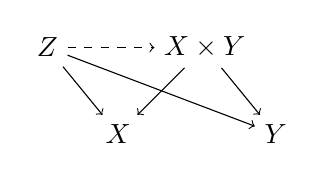
\begin{tikzpicture}[baseline=(current bounding box.center)]
\node (Z) at (0,1.1) {$Z$};
\node (P) at (2.0,1.1) {$X\times Y$};
\node (X) at (.9,0) {$X$};
\node (Y) at (2.9,0) {$Y$};
\draw[->,dashed] (Z)--(P);
\draw[->] (Z)--(X);
\draw[->] (Z)--(Y);
\draw[->] (P)--(X);
\draw[->] (P)--(Y);
\end{tikzpicture}
\]

(d) Show that $\dim X\times Y=\dim X+\dim Y$.

\smallskip
\noindent\hypertarget{ex-I-3.16}{}\textbf{3.16.}\enspace \emph{Products of Quasi-Projective Varieties.} Use the Segre embedding (Ex.~\Goto{ex-I-2.14}{2.14}) to identify $\Proj^n\times\Proj^m$ with its image and hence give it a structure of projective variety. Now for any two quasi-projective varieties $X\subseteq\Proj^n$ and $Y\subseteq\Proj^m$, consider $X\times Y\subseteq\Proj^n\times\Proj^m$.

(a) Show that $X\times Y$ is a quasi-projective variety.

(b) If $X,Y$ are both projective, show that $X\times Y$ is projective.

*(c) Show that $X\times Y$ is a product in the category of varieties.%
}
% Contents from body/page-037.tex.
\ChapterSheet{37}{23}{3\quad Morphisms}{%
\fontsize{9}{10.75}\selectfont\setlength{\parskip}{.75pt}
\noindent\hypertarget{ex-I-3.17}{}\textbf{3.17.}\enspace \emph{Normal Varieties.} A variety $Y$ is \emph{normal at a point} $P\in Y$ if $\mathcal O_P$ is an integrally closed ring. $Y$ is \emph{normal} if it is normal at every point.

(a) Show that every conic in $\Proj^2$ is normal.

(b) Show that the quadric surfaces $Q_1,Q_2$ in $\Proj^3$ given by equations $Q_1\colon xy=zw$; $Q_2\colon xy=z^2$ are normal (cf. (II, Ex.~\Goto{ex-II-6.4}{6.4}) for the latter.)

(c) Show that the cuspidal cubic $y^2=x^3$ in $\AffSpace{2}$ is not normal.

(d) If $Y$ is affine, then $Y$ is normal $\Leftrightarrow A(Y)$ is integrally closed.

(e) Let $Y$ be an affine variety. Show that there is a normal affine variety $\widetilde Y$, and a morphism $\pi\colon\widetilde Y\to Y$, with the property that whenever $Z$ is a normal variety, and $\varphi\colon Z\to Y$ is a \emph{dominant} morphism (i.e., $\varphi(Z)$ is dense in $Y$), then there is a unique morphism $\theta\colon Z\to\widetilde Y$ such that $\varphi=\pi\circ\theta$. $\widetilde Y$ is called the \emph{normalization} of $Y$. You will need \Goto{result-I-3.9A}{(3.9A)} above.

\smallskip
\noindent\hypertarget{ex-I-3.18}{}\textbf{3.18.}\enspace \emph{Projectively Normal Varieties.} A projective variety $Y\subseteq\Proj^n$ is \emph{projectively normal} (with respect to the given embedding) if its homogeneous coordinate ring $S(Y)$ is integrally closed.

(a) If $Y$ is projectively normal, then $Y$ is normal.

(b) There are normal varieties in projective space which are not projectively normal. For example, let $Y$ be the twisted quartic curve in $\Proj^3$ given parametrically by $(x,y,z,w)=(t^4,t^3u,tu^3,u^4)$. Then $Y$ is normal but not projectively normal. See (III, Ex.~\Goto{ex-III-5.6}{5.6}) for more examples.

(c) Show that the twisted quartic curve $Y$ above is isomorphic to $\Proj^1$, which is projectively normal. Thus projective normality depends on the embedding.

\smallskip
\noindent\hypertarget{ex-I-3.19}{}\textbf{3.19.}\enspace \emph{Automorphisms of $\AffSpace{n}$.} Let $\varphi\colon\AffSpace{n}\to\AffSpace{n}$ be a morphism of $\AffSpace{n}$ to $\AffSpace{n}$ given by $n$ polynomials $f_1,\ldots,f_n$ of $n$ variables $x_1,\ldots,x_n$. Let $J=\det\lvert\partial f_i/\partial x_j\rvert$ be the \emph{Jacobian} polynomial of $\varphi$.

(a) If $\varphi$ is an isomorphism (in which case we call $\varphi$ an \emph{automorphism} of $\AffSpace{n}$) show that $J$ is a nonzero constant polynomial.

**(b) \hypertarget{err-I-3.19}{}\EditionText{In characteristic zero and for $n=2$, the converse of (a) is an unsolved problem.} See, for example, Vitushkin \Goto{bib-vitushkin-1-item-1}{[1]}.

\smallskip
\noindent\hypertarget{ex-I-3.20}{}\textbf{3.20.}\enspace Let $Y$ be a variety of dimension $\geqslant2$, and let $P\in Y$ be a normal point. Let $f$ be a regular function on $Y-P$.

(a) Show that $f$ extends to a regular function on $Y$.

(b) Show this would be false for $\dim Y=1$.

See (III, Ex.~\Goto{ex-III-3.5}{3.5}) for generalization.

\smallskip
\noindent\hypertarget{ex-I-3.21}{}\textbf{3.21.}\enspace \emph{Group Varieties.} A \emph{group variety} consists of a variety $Y$ together with a morphism $\mu\colon Y\times Y\to Y$, such that the set of points of $Y$ with the operation given by $\mu$ is a group, and such that the inverse map $y\mapsto y^{-1}$ is also a morphism of $Y\to Y$.

(a) The \emph{additive group} $G_a$ is given by the variety $\AffSpace{1}$ and the morphism $\mu\colon\AffSpace{2}\to\AffSpace{1}$ defined by $\mu(a,b)=a+b$. Show it is a group variety.

(b) The \emph{multiplicative group} $G_m$ is given by the variety $\AffSpace{1}-\{(0)\}$ and the morphism $\mu(a,b)=ab$. Show it is a group variety.

(c) If $G$ is a group variety, and $X$ is any variety, show that the set $\operatorname{Hom}(X,G)$ has a natural group structure.

(d) For any variety $X$, show that $\operatorname{Hom}(X,G_a)$ is isomorphic to $\mathcal O(X)$ as a group under addition.

(e) For any variety $X$, show that $\operatorname{Hom}(X,G_m)$ is isomorphic to the group of units in $\mathcal O(X)$, under multiplication.%
}
% Contents from body/page-038.tex.
\BookMark{1}{1.4 Rational Maps}{sec-I-4}
\ChapterSheet{38}{24}{I\quad Varieties}{%
\noindent\hypertarget{sec-I-4}{}\textbf{\large 4\enspace Rational Maps}

\smallskip
In this section we introduce the notions of rational map and birational equivalence, which are important for the classification of varieties. A rational map is a morphism which is only defined on some open subset. Since an open subset of a variety is dense, this already carries a lot of information. In this respect algebraic geometry is more \textquotedblleft{}rigid\textquotedblright{} than differential geometry or topology. In particular, the concept of birational equivalence is unique to algebraic geometry.

\smallskip
\noindent\hypertarget{result-I-4.1}{}\textbf{Lemma 4.1.}\enspace \textit{Let $X$ and $Y$ be varieties, let $\varphi$ and $\psi$ be two morphisms from $X$ to $Y$, and suppose there is a nonempty open subset $U\subseteq X$ such that $\varphi|_U=\psi|_U$. Then $\varphi=\psi$.}

\smallskip
\noindent\textsc{Proof.}\enspace We may assume that $Y\subseteq\Proj^n$ for some $n$. Then by composing with the inclusion morphism $Y\to\Proj^n$, we reduce to the case $Y=\Proj^n$. We consider the product $\Proj^n\times\Proj^n$, which has a structure of projective variety given by its Segre embedding (Ex.~\Goto{ex-I-3.16}{3.16}). The morphisms $\varphi$ and $\psi$ determine a map $\varphi\times\psi\colon X\to\Proj^n\times\Proj^n$, which in fact is a morphism (Ex.~\Goto{ex-I-3.16}{3.16c}). Let $\Delta=\{P\times P\mid P\in\Proj^n\}$ be the \emph{diagonal} subset of $\Proj^n\times\Proj^n$. It is defined by the equations $\{x_i y_j=x_j y_i\mid i,j=0,1,\ldots,n\}$ and so is a closed subset of $\Proj^n\times\Proj^n$. By hypothesis $\varphi\times\psi(U)\subseteq\Delta$. But $U$ is dense in $X$, and $\Delta$ is closed, so $\varphi\times\psi(X)\subseteq\Delta$. This says that $\varphi=\psi$.

\smallskip
\noindent\textbf{Definition.}\enspace Let $X,Y$ be varieties. A \emph{rational map} $\varphi\colon X\to Y$ is an equivalence class of pairs $\langle U,\varphi_U\rangle$ where $U$ is a nonempty open subset of $X$, $\varphi_U$ is a morphism of $U$ to $Y$, and where $\langle U,\varphi_U\rangle$ and $\langle V,\varphi_V\rangle$ are equivalent if $\varphi_U$ and $\varphi_V$ agree on $U\cap V$. The rational map $\varphi$ is \emph{dominant} if for some (and hence every) pair $\langle U,\varphi_U\rangle$, the image of $\varphi_U$ is dense in $Y$.

\smallskip
Note that the lemma implies that the relation on pairs $\langle U,\varphi_U\rangle$ just described is an equivalence relation. Note also that a rational map $\varphi\colon X\to Y$ is \emph{not} in general a map of the set $X$ to $Y$. Clearly one can compose \emph{dominant} rational maps, so we can consider the category of varieties and dominant rational maps. An \textquotedblleft{}isomorphism\textquotedblright{} in this category is called a birational map:

\smallskip
\noindent\textbf{Definition.}\enspace A \emph{birational map} $\varphi\colon X\to Y$ is a rational map which admits an inverse, namely a rational map $\psi\colon Y\to X$ such that $\psi\circ\varphi=\operatorname{id}_X$ and $\varphi\circ\psi=\operatorname{id}_Y$ as rational maps. If there is a birational map from $X$ to $Y$, we say that $X$ and $Y$ are \emph{birationally equivalent}, or simply \emph{birational}.

\smallskip
The main result of this section is that the category of varieties and dominant rational maps is equivalent to the category of finitely generated field%
}
% Contents from body/page-039.tex.
\ChapterSheet{39}{25}{4\quad Rational Maps}{%
\noindent extensions of $k$, with the arrows reversed. Before giving this result, we need a couple of lemmas which show that on any variety, the open affine subsets form a base for the topology. We say loosely that a variety is \emph{affine} if it is isomorphic to an affine variety.

\smallskip
\noindent\hypertarget{result-I-4.2}{}\textbf{Lemma 4.2.}\enspace \textit{Let $Y$ be a hypersurface in $\AffSpace{n}$ given by the equation $f(x_1,\ldots,x_n)=0$. Then $\AffSpace{n}-Y$ is isomorphic to the hypersurface $H$ in $\AffSpace{n+1}$ given by $x_{n+1}f=1$. In particular, $\AffSpace{n}-Y$ is affine, and its affine ring is $k[x_1,\ldots,x_n]_f$.}

\smallskip
\noindent\textsc{Proof.}\enspace For $P=(a_1,\ldots,a_{n+1})\in H$, let $\varphi(P)=(a_1,\ldots,a_n)$. Then clearly $\varphi$ is a morphism from $H$ to $\AffSpace{n}$, corresponding to the homomorphism of rings $A\to A_f$, where $A=k[x_1,\ldots,x_n]$. It is also clear that $\varphi$ gives a bijective mapping of $H$ onto its image, which is $\AffSpace{n}-Y$. To show that $\varphi$ is an isomorphism, it is sufficient to show that $\varphi^{-1}$ is a morphism. But $\varphi^{-1}(a_1,\ldots,a_n)=(a_1,\ldots,a_n,1/f(a_1,\ldots,a_n))$, so the fact that $\varphi^{-1}$ is a morphism on $\AffSpace{n}-Y$ follows from \Goto{result-I-3.6}{(3.6)}.

\smallskip
\noindent\hypertarget{result-I-4.3}{}\textbf{Proposition 4.3.}\enspace \textit{On any variety $Y$, there is a base for the topology consisting of open affine subsets.}

\smallskip
\noindent\textsc{Proof.}\enspace We must show for any point $P\in Y$ and any open set $U$ containing $P$, that there exists an open affine set $V$ with $P\in V\subseteq U$. First, since $U$ is also a variety, we may assume $U=Y$. Secondly, since any variety is covered by quasi-affine varieties \Goto{result-I-2.3}{(2.3)}, we may assume that $Y$ is quasi-affine in $\AffSpace{n}$. Let $Z=\overline Y-Y$, which is a closed set in $\AffSpace{n}$, and let $\mathfrak a\subseteq A=k[x_1,\ldots,x_n]$ be the ideal of $Z$. Then, since $Z$ is closed, and $P\notin Z$, we can find a polynomial $f\in\mathfrak a$ such that $f(P)\ne0$. Let $H$ be the hypersurface $f=0$ in $\AffSpace{n}$. Then $Z\subseteq H$ but $P\notin H$. Thus $P\in Y-Y\cap H$, which is an open subset of $Y$. Furthermore, $Y-Y\cap H$ is a closed subset of $\AffSpace{n}-H$, which is affine by \Goto{result-I-4.2}{(4.2)}, hence $Y-Y\cap H$ is affine. This is the required affine neighborhood of $P$.

\smallskip
Now we come to the main result of this section. Let $\varphi\colon X\to Y$ be a dominant rational map, represented by $\langle U,\varphi_U\rangle$. Let $f\in K(Y)$ be a rational function, represented by $\langle V,f\rangle$ where $V$ is an open set in $Y$, and $f$ is a regular function on $V$. Since $\varphi_U(U)$ is dense in $Y$, $\varphi_U^{-1}(V)$ is a nonempty open subset of $X$, so $f\circ\varphi_U$ is a regular function on $\varphi_U^{-1}(V)$. This gives us a rational function on $X$, and in this manner we have defined a homomorphism of $k$-algebras from $K(Y)$ to $K(X)$.

\smallskip
\noindent\hypertarget{result-I-4.4}{}\textbf{Theorem 4.4.}\enspace {\itshape For any two varieties $X$ and $Y$, the above construction gives a bijection between

(i) the set of dominant rational maps from $X$ to $Y$, and

(ii) the set of $k$-algebra homomorphisms from $K(Y)$ to $K(X)$.}%
}
% Contents from body/page-040.tex.
\ChapterSheet{40}{26}{I\quad Varieties}{%
\noindent\textit{Furthermore, this correspondence gives an arrow-reversing equivalence of categories of the category of varieties and dominant rational maps with the category of finitely generated field extensions of $k$.}

\smallskip
\noindent\textsc{Proof.}\enspace We will construct an inverse to the mapping given by the construction above. Let $\theta\colon K(Y)\to K(X)$ be a homomorphism of $k$-algebras. We wish to define a rational map from $X$ to $Y$. By \Goto{result-I-4.3}{(4.3)}, $Y$ is covered by affine varieties, so we may assume $Y$ is affine. Let $A(Y)$ be its affine coordinate ring, and let $y_1,\ldots,y_n$ be generators for $A(Y)$ as a $k$-algebra. Then $\theta(y_1),\ldots,\theta(y_n)$ are rational functions on $X$. We can find an open set $U\subseteq X$ such that the functions $\theta(y_i)$ are all regular on $U$. Then $\theta$ defines an injective homomorphism of $k$-algebras $A(Y)\to\mathcal O(U)$. By \Goto{result-I-3.5}{(3.5)} this corresponds to a morphism $\varphi\colon U\to Y$, which gives us a dominant rational map from $X$ to $Y$. It is easy to see that this gives a map of sets (ii) $\to$ (i) which is inverse to the one defined above.

To see that we have an equivalence of categories as stated, we need only check that for any variety $Y$, $K(Y)$ is finitely generated over $k$, and conversely, if $K/k$ is a finitely generated field extension, then $K=K(Y)$ for some $Y$. If $Y$ is a variety, then $K(Y)=K(U)$ for any open affine subset, so we may assume $Y$ affine. Then by \Goto{result-I-3.2}{(3.2d)}, $K(Y)$ is a finitely generated field extension of $k$. On the other hand, let $K$ be a finitely generated field extension of $k$. Let $y_1,\ldots,y_n\in K$ be a set of generators, and let $B$ be the sub-$k$-algebra of $K$ generated by $y_1,\ldots,y_n$. Then $B$ is a quotient of the polynomial ring $A=k[x_1,\ldots,x_n]$, so $B\cong A(Y)$ for some variety $Y$ in $\AffSpace{n}$. Then $K\cong K(Y)$ so we are done.

\smallskip
\noindent\hypertarget{result-I-4.5}{}\textbf{Corollary 4.5.}\enspace {\itshape For any two varieties $X,Y$ the following conditions are equivalent:

(i) $X$ and $Y$ are birationally equivalent;

(ii) there are \hypertarget{err-I-4.5}{}\EditionText{nonempty }open subsets $U\subseteq X$ and $V\subseteq Y$ with $U$ isomorphic to $V$,

(iii) $K(X)\cong K(Y)$ as $k$-algebras.}

\smallskip
\noindent\textsc{Proof.}

(i) $\Rightarrow$ (ii). Let $\varphi\colon X\to Y$ and $\psi\colon Y\to X$ be rational maps which are inverse to each other. Let $\varphi$ be represented by $\langle U,\varphi\rangle$ and let $\psi$ be represented by $\langle V,\psi\rangle$. Then $\psi\circ\varphi$ is represented by $\langle\varphi^{-1}(V),\psi\circ\varphi\rangle$, and since $\psi\circ\varphi=\operatorname{id}_X$ as a rational map, $\psi\circ\varphi$ is the identity on $\varphi^{-1}(V)$. Similarly $\varphi\circ\psi$ is the identity on $\psi^{-1}(U)$. We now take $\varphi^{-1}(\psi^{-1}(U))$ as our open set in $X$, and $\psi^{-1}(\varphi^{-1}(V))$ as our open set in $Y$. It follows from the construction that these two open sets are isomorphic via $\varphi$ and $\psi$.

(ii) $\Rightarrow$ (iii) follows from the definition of function field.

(iii) $\Rightarrow$ (i) follows from the theorem.

\smallskip
As an illustration of the notion of birational correspondence, we will use some algebraic results on field extensions to show that every variety is bi-%
}
% Contents from body/page-041.tex.
\ChapterSheet{41}{27}{4\quad Rational Maps}{%
\noindent rational to a hypersurface. We assume familiarity with the notion of separable algebraic field extensions, and the notions of transcendence base and transcendence degree for infinite field extensions (see, e.g., Zariski--Samuel \Goto{legacy-b-zs}{[1, Ch.~II]}).

\smallskip
\noindent\hypertarget{result-I-4.6A}{}\textbf{Theorem 4.6A} (Theorem of the Primitive Element). \textit{Let $L$ be a finite separable extension field of a field $K$. Then there is an element $\alpha\in L$ which generates $L$ as an extension field of $K$. Furthermore, if $\beta_1,\ldots,\beta_n$ is any set of generators of $L$ over $K$, and if $K$ is infinite, then $\alpha$ can be taken to be a linear combination $\alpha=c_1\beta_1+\cdots+c_n\beta_n$ of the $\beta_i$ with coefficients $c_i\in K$.}

\smallskip
\noindent\textsc{Proof.}\enspace Zariski--Samuel \Goto{legacy-b-zs}{[1, Ch.~II, Theorem 19, p.~84]}. The second statement follows from the proof given there.

\smallskip
\noindent\textbf{Definition.}\enspace A field extension $K/k$ is \emph{separably generated} if there is a transcendence base $\{x_i\}$ for $K/k$ such that $K$ is a separable algebraic extension of $k(\{x_i\})$. Such a transcendence base is called a \emph{separating transcendence base}.

\smallskip
\noindent\hypertarget{result-I-4.7A}{}\textbf{Theorem 4.7A.}\enspace \textit{If a field extension $K/k$ is finitely generated and separably generated, then any set of generators contains a subset which is a separating transcendence base.}

\smallskip
\noindent\textsc{Proof.}\enspace Zariski--Samuel \Goto{legacy-b-zs}{[1, Ch.~II, Theorem 30, p.~104]}.

\smallskip
\noindent\hypertarget{result-I-4.8A}{}\textbf{Theorem 4.8A.}\enspace \textit{If $k$ is a perfect field (hence in particular if $k$ is algebraically closed), any finitely generated field extension $K/k$ is separably generated.}

\smallskip
\noindent\textsc{Proof.}\enspace Zariski--Samuel \Goto{legacy-b-zs}{[1, Ch.~II, Theorem 31, p.~105]}, or Matsumura \Goto{legacy-b-mat}{[2, Ch.~10, Corollary, p.~194]}.

\smallskip
\noindent\hypertarget{result-I-4.9}{}\textbf{Proposition 4.9.}\enspace \textit{Any variety $X$ of dimension $r$ is birational to a hypersurface $Y$ in $\Proj^{r+1}$.}

\smallskip
\noindent\textsc{Proof.}\enspace The function field $K$ of $X$ is a finitely generated extension field of $k$. By \Goto{result-I-4.8A}{(4.8A)}, $K$ is separably generated over $k$. Hence we can find a transcendence base $x_1,\ldots,x_r\in K$ such that $K$ is a finite separable extension of $k(x_1,\ldots,x_r)$. Then by \Goto{result-I-4.6A}{(4.6A)} we can find one further element $y\in K$ such that $K=k(x_1,\ldots,x_r,y)$. Now $y$ is algebraic over $k(x_1,\ldots,x_r)$, so it satisfies a \hypertarget{err-I-4.9}{}\EditionText{minimal polynomial equation} with coefficients which are rational functions in $x_1,\ldots,x_r$. Clearing denominators\EditionText{ and removing the common factor of the coefficients}, we get an irreducible polynomial $f(x_1,\ldots,x_r,y)=0$. This defines a hypersurface in $\AffSpace{r+1}$ with function field $K$, which, according to \Goto{result-I-4.5}{(4.5)}, is birational to $X$. Its projective closure (Ex.~\Goto{ex-I-2.9}{2.9}) is the required hypersurface $Y\subseteq\Proj^{r+1}$.%
}
% Contents from body/page-042.tex.
\ChapterSheet{42}{28}{I\quad Varieties}{%
\noindent\emph{Blowing Up}

\smallskip
As another example of a birational map, we will now construct the blowing-up of a variety at a point. This important construction is the main tool in the resolution of singularities of an algebraic variety.

First we will construct the blowing-up of $\AffSpace{n}$ at the point $O=(0,\ldots,0)$. Consider the product $\AffSpace{n}\times\Proj^{n-1}$, which is a quasi-projective variety (Ex.~\Goto{ex-I-3.16}{3.16}). If $x_1,\ldots,x_n$ are the affine coordinates of $\AffSpace{n}$, and if $y_1,\ldots,y_n$ are the homogeneous coordinates of $\Proj^{n-1}$ (observe the unusual notation!), then the closed subsets of $\AffSpace{n}\times\Proj^{n-1}$ are defined by polynomials in the $x_i,y_j$, which are homogeneous with respect to the $y_j$.

We now define the \emph{blowing-up of $\AffSpace{n}$ at the point $O$} to be the closed subset $X$ of $\AffSpace{n}\times\Proj^{n-1}$ defined by the equations $\{x_i y_j=x_j y_i\mid i,j=1,\ldots,n\}$.
\[
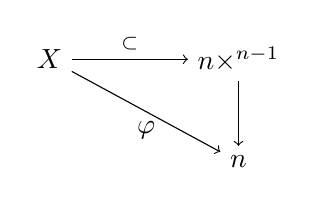
\begin{tikzpicture}[baseline=(current bounding box.center)]
\node (X) at (0,1.3) {$X$};
\node (P) at (2.4,1.3) {$\AffSpace{n}\times\Proj^{n-1}$};
\node (A) at (2.4,0) {$\AffSpace{n}$};
\draw[->] (X)--node[above] {$\scriptstyle\subset$} (P);
\draw[->] (X)--node[below] {$\varphi$} (A);
\draw[->] (P)--(A);
\end{tikzpicture}
\]
We have a natural morphism $\varphi\colon X\to\AffSpace{n}$ obtained by restricting the projection map of $\AffSpace{n}\times\Proj^{n-1}$ onto the first factor. We will now study the properties of $X$.

(1) If $P\in\AffSpace{n}$, $P\ne O$, then $\varphi^{-1}(P)$ consists of a single point. In fact, $\varphi$ gives an isomorphism of $X-\varphi^{-1}(O)$ onto $\AffSpace{n}-O$. Indeed, let $P=(a_1,\ldots,a_n)$, with some $a_i\ne0$. Now if $P\times(y_1,\ldots,y_n)\in\varphi^{-1}(P)$, then for each $j$, $y_j=(a_j/a_i)y_i$, so $(y_1,\ldots,y_n)$ is uniquely determined as a point in $\Proj^{n-1}$. In fact, setting $y_i=a_i$, we can take $(y_1,\ldots,y_n)=(a_1,\ldots,a_n)$. Thus $\varphi^{-1}(P)$ consists of a single point. Furthermore, for $P\in\AffSpace{n}-O$, setting $\psi(P)=(a_1,\ldots,a_n)\times(a_1,\ldots,a_n)$ defines an inverse morphism to $\varphi$, showing $X-\varphi^{-1}(O)$ is isomorphic to $\AffSpace{n}-O$.

(2) $\varphi^{-1}(O)\cong\Proj^{n-1}$. Indeed, $\varphi^{-1}(O)$ consists of all points $O\times Q$, with $Q=(y_1,\ldots,y_n)\in\Proj^{n-1}$, subject to no restriction.

(3) The points of $\varphi^{-1}(O)$ are in $1$-$1$ correspondence with the set of lines through $O$ in $\AffSpace{n}$. Indeed, a line $L$ through $O$ in $\AffSpace{n}$ can be given by parametric equations $x_i=a_i t$, $i=1,\ldots,n$, where $a_i\in k$ are not all zero, and $t\in\AffSpace{1}$. Now consider the line $L'=\varphi^{-1}(L-O)$ in $X-\varphi^{-1}(O)$. It is given parametrically by $x_i=a_i t$, $y_i=a_i t$, with $t\in\AffSpace{1}-O$. But the $y_i$ are homogeneous coordinates in $\Proj^{n-1}$, so we can equally well describe $L'$ be the equations $x_i=a_i t,y_i=a_i$, for $t\in\AffSpace{1}-O$. These equations make sense also for $t=0$, and give the closure $\overline{L'}$ of $L'$ in $X$. Now $\overline{L'}$ meets $\varphi^{-1}(O)$ in the point $Q=(a_1,\ldots,a_n)\in\Proj^{n-1}$, so we see that sending $L$ to $Q$ gives a $1$-$1$ correspondence between lines through $O$ in $\AffSpace{n}$ and points of $\varphi^{-1}(O)$.

(4) $X$ is irreducible. Indeed, $X$ is the union of $X-\varphi^{-1}(O)$ and $\varphi^{-1}(O)$. The first piece is isomorphic to $\AffSpace{n}-O$, hence irreducible. On the other hand, we have just seen that every point of $\varphi^{-1}(O)$ is in the closure of some%
}
% Contents from body/page-043.tex.
\ChapterSheet{43}{29}{4\quad Rational Maps}{%
{\centering
\noindent\hypertarget{fig-book-3}{}\par\nobreak\noindent\resizebox{.97\linewidth}{!}{% Figure 3. Blowing up (printed page 29).
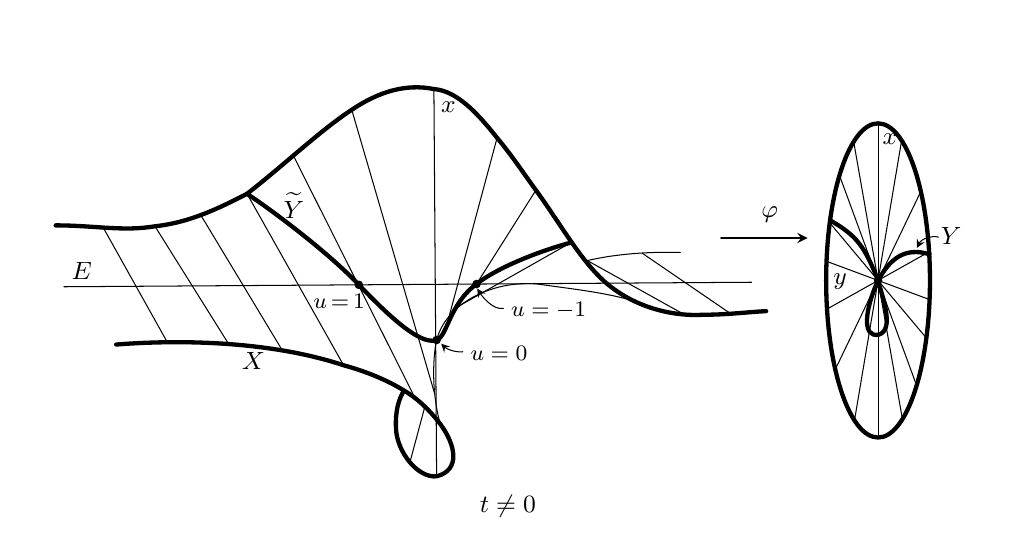
\begin{tikzpicture}[
    x=.325bp, y=-.325bp,
    line cap=round, line join=round, >=stealth,
    ruling/.style={line width=.37bp},
    contour/.style={line width=1.55bp},
    every node/.style={inner sep=0pt, font=\small}
  ]
  \path[use as bounding box] (-25,-14) rectangle (1048.846,535.538);

  \coordinate (turn) at (428,332);
  \coordinate (left-tip) at (218,170);
  \coordinate (right-tip) at (577,224);
  \coordinate (fold) at (392,388);

  % Exceptional curve, x-direction, and straight rulings on X.
  \draw[ruling] (15,273) -- coordinate[pos=.429] (positive)
    coordinate[pos=.600] (negative) (777,268);
  \draw[ruling] (425,54) -- (428,483);
  % The fold hides this ruling between its two visible pieces.
  \path (495,108) -- coordinate[pos=.600] (ruling-hidden)
    coordinate[pos=.824] (ruling-visible) (398,469);
  \draw[ruling]
    (59,208) -- (130,335)
    (116,206) -- (198,337)
    (167,194) -- (258,345)
    (left-tip) -- (325,360)
    (270,129) -- (405,398)
    (334,77) -- (426,392)
    (495,108) -- (ruling-hidden)
    (ruling-visible) -- (398,469)
    (538,166) -- (negative)
    (right-tip) -- (448,297)
    (595,244) -- (701,303)
    (656,236) -- (754,303);
  \draw[ruling]
    (fold) -- (384,405)
    (432,425) .. controls (422,389) and (424,350) .. (turn)
      .. controls (440,286) and (501,263) .. (547,271)
      .. controls (583,276) and (618,280) .. (647,289)
    (595,244) .. controls (625,237) and (660,234) .. (698,235);

  % Upper and lower rims of X, and the strict transform of Y.
  \draw[contour]
    (6,205) .. controls (49,205) and (81,212) .. (116,206)
    .. controls (154,202) and (187,186) .. (left-tip)
    .. controls (258,139) and (300,99) .. (334,77)
    .. controls (365,56) and (395,48) .. (425,54)
    .. controls (453,56) and (478,87) .. (495,108)
    .. controls (514,131) and (524,147) .. (538,166)
    .. controls (565,203) and (588,245) .. (616,269)
    .. controls (649,297) and (691,306) .. (724,304)
    .. controls (750,304) and (773,301) .. (793,300);
  \draw[contour]
    (73,337) .. controls (164,330) and (256,337) .. (325,360)
    .. controls (351,367) and (374,377) .. (fold)
    .. controls (409,398) and (423,413) .. (432,425)
    .. controls (449,448) and (455,476) .. (428,483)
    .. controls (407,485) and (384,456) .. (383,430)
    .. controls (382,411) and (386,397) .. (fold);
  \draw[contour]
    (left-tip) .. controls (251,192) and (310,237) .. (positive)
    .. controls (370,300) and (409,339) .. (turn)
    .. controls (440,328) and (442,292) .. (negative)
    .. controls (495,252) and (540,234) .. (right-tip);

  \fill (positive) circle[radius=1.55bp];
  \fill (negative) circle[radius=1.55bp];
  \fill (turn) circle[radius=1.55bp];
  \node at (441,74) {$x$};
  \node at (270,183) {$\widetilde{Y}$};
  \node at (35,256) {$E$};
  \node[font=\footnotesize] at (320,289) {$u\,{=}\,1$};
  \node[anchor=west,font=\footnotesize] at (510,299) {$u=-1$};
  \node[anchor=west,font=\footnotesize] at (465,347) {$u=0$};
  \node at (225,355) {$X$};
  \node at (507,516) {$t\ne 0$};
  \draw[ruling,->] (502,297)
    .. controls (490,299) and (478,283) .. (473,275);
  \draw[ruling,->] (457,345)
    .. controls (447,346) and (438,341) .. (433,336);

  \draw[->,line width=.65bp] (743,219) -- (839,219);
  \node at (797,193) {$\varphi$};

  % Target: the directions through the node of the plane cubic.
  \coordinate (O) at (917,266);
  \foreach \angle in {7,21.5,42,62,90,117,145.5,169.5} {
    \pgfmathsetmacro{\dx}{57.5*cos(\angle)}
    \pgfmathsetmacro{\dy}{174*sin(\angle)}
    \draw[ruling] (O) ++({-\dx},{-\dy}) -- ++({2*\dx},{2*\dy});
  }
  \draw[contour] (O) ellipse[x radius=57.5, y radius=174];
  \draw[contour]
    (864,199.5) .. controls (893,216) and (902,228) .. (O)
    .. controls (921,282) and (936,320) .. (918,326)
    .. controls (899,330) and (902,299) .. (O)
    .. controls (931,241) and (947,229) .. (974,237);
  \fill (O) circle[radius=1.55bp];
  \node at (930,110) {$x$};
  \node at (875,267) {$y$};
  \node[anchor=west] at (986,217) {$Y$};
  \draw[ruling,->] (984,218)
    .. controls (976,216) and (965,220) .. (960,230);
\end{tikzpicture}
}\par
\small\textbf{Figure 3.}\enspace Blowing up.\par}

\smallskip
\noindent subset (the line $L'$) of $X-\varphi^{-1}(O)$. Hence $X-\varphi^{-1}(O)$ is dense in $X$, and $X$ is irreducible.

\smallskip
\noindent\textbf{Definition.}\enspace If $Y$ is a closed subvariety of $\AffSpace{n}$ passing through $O$, we define the \emph{blowing-up of $Y$ at the point $O$} to be $\widetilde Y=\overline{\varphi^{-1}(Y-O)}$, where $\varphi\colon X\to\AffSpace{n}$ is the blowing-up of $\AffSpace{n}$ at the point $O$ described above. We denote also by $\varphi\colon\widetilde Y\to Y$ the morphism obtained by restricting $\varphi\colon X\to\AffSpace{n}$ to $\widetilde Y$. To blow up at any other point $P$ of $\AffSpace{n}$, \hypertarget{err-I-4-translation}{}\EditionText{translate the coordinates to send $P$ to $O$.}

\smallskip
Note that $\varphi$ induces an isomorphism of $\widetilde Y-\varphi^{-1}(O)$ to $Y-O$, so that \hypertarget{err-I-4-blowup-point}{}\EditionText{if $Y\ne\{O\}$, }$\varphi$ is a birational morphism of $\widetilde Y$ to $Y$. Note also that this definition apparently depends on the embedding of $Y$ in $\AffSpace{n}$, but in fact, we will see later that blowing-up is intrinsic \Goto{result-II-7.15.1}{(II, 7.15.1)}.

The effect of blowing up a point of $Y$ is to \textquotedblleft{}pull apart\textquotedblright{} $Y$ near $O$ according to the different directions of lines through $O$. We will illustrate this with an example.

\smallskip
\noindent\hypertarget{result-I-4.9.1}{}\textbf{Example 4.9.1.}\enspace \hypertarget{err-I-4.9.1}{}\EditionText{Assume that $\operatorname{char} k\ne2$. }Let $Y$ be the plane cubic curve given by the equation $y^2=x^2(x+1)$. We will blow up $Y$ at $O$ (Fig.~\Goto{fig-book-3}{3}). Let $t,u$ be homogeneous coordinates for $\Proj^1$. Then $X$, the blowing-up of $\AffSpace{2}$ at $O$, is defined by the equation $xu=ty$ inside $\AffSpace{2}\times\Proj^1$. It looks like $\AffSpace{2}$, except that the point $O$ has been replaced by a $\Proj^1$ corresponding to the slopes of lines through $O$. We will call this $\Proj^1$ the \emph{exceptional curve}, and denote it by $E$.

We obtain the total inverse image of $Y$ in $X$ by considering the equations $y^2=x^2(x+1)$ and $xu=ty$ in $\AffSpace{2}\times\Proj^1$. Now $\Proj^1$ is covered by the open sets $t\ne0$ and $u\ne0$, which we consider separately. If $t\ne0$, we can set $t=1$, and use $u$ as an affine parameter. Then we have the equations
\[
\begin{gathered}
y^2=x^2(x+1)\\
y=xu
\end{gathered}
\]%
}
% Contents from body/page-044.tex.
\ChapterSheet{44}{30}{I\quad Varieties}{%
\noindent in $\AffSpace{3}$ with coordinates $x,y,u$. Substituting, we get $x^2u^2-x^2(x+1)=0$, which factors. Thus we obtain two irreducible components, one defined by $x=0,y=0,u$ arbitrary, which is $E$, and the other defined by $u^2=x+1,y=xu$. This is $\widetilde Y$. Note that $\widetilde Y$ meets $E$ at the points $u=\pm1$. These points correspond to the slopes of the two branches of $Y$ at $O$.

Similarly one can check that the total inverse image of the $x$-axis consists of $E$ and one other irreducible curve, which we call the \emph{strict transform of the $x$-axis} (it is the curve $\overline{L'}$ described earlier corresponding to the line $L=x$-axis). This strict transform meets $E$ at the point $u=0$. By considering the other open set $u\ne0$ in $\AffSpace{2}\times\Proj^1$, one sees that the strict transform of the $y$-axis meets $E$ at the point $t=0,u=1$.

These conclusions are summarized in Figure~\Goto{fig-book-3}{3}. The effect of blowing up is thus to separate out branches of curves passing through $O$ according to their slopes. If the slopes are different, their strict transforms \hypertarget{err-I-4-meet-over-center}{}\EditionText{do not meet over $O$.} Instead, they meet $E$ at points corresponding to the different slopes.

\smallskip
\noindent\textsc{Exercises}

\begingroup\small
\noindent\hypertarget{ex-I-4.1}{}\textbf{4.1.}\enspace If $f$ and $g$ are regular functions on open subsets $U$ and $V$ of a variety $X$, and if $f=g$ on $U\cap V$, show that the function which is $f$ on $U$ and $g$ on $V$ is a regular function on $U\cup V$. Conclude that if $f$ is a rational function on $X$, then there is a largest open subset $U$ of $X$ on which $f$ is represented by a regular function. We say that $f$ is \emph{defined} at the points of $U$.

\smallskip
\noindent\hypertarget{ex-I-4.2}{}\textbf{4.2.}\enspace Same problem for rational maps. If $\varphi$ is a rational map of $X$ to $Y$, show there is a largest open set on which $\varphi$ is represented by a morphism. We say the rational map is \emph{defined} at the points of that open set.

\smallskip
\noindent\hypertarget{ex-I-4.3}{}\textbf{4.3.}\enspace (a) Let $f$ be the rational function on $\Proj^2$ given by $f=x_1/x_0$. Find the set of points where $f$ is defined and describe the corresponding regular function.

(b) Now think of this function as a rational map from $\Proj^2$ to $\AffSpace{1}$. Embed $\AffSpace{1}$ in $\Proj^1$, and let $\varphi\colon\Proj^2\to\Proj^1$ be the resulting rational map. Find the set of points where $\varphi$ is defined, and describe the corresponding morphism.

\smallskip
\noindent\hypertarget{ex-I-4.4}{}\textbf{4.4.}\enspace A variety $Y$ is \emph{rational} if it is birationally equivalent to $\Proj^n$ for some $n$ (or, equivalently by \Goto{result-I-4.5}{(4.5)}, if $K(Y)$ is a pure transcendental extension of $k$).

(a) Any conic in $\Proj^2$ is a rational curve.

(b) The cuspidal cubic $y^2=x^3$ is a rational curve.

(c) Let $Y$ be the \hypertarget{err-I-4.4c}{}\EditionText{cubic curve} $y^2z=x^2(x+z)$ in $\Proj^2$\EditionText{ (nodal if $\operatorname{char} k\ne2$)}. Show that the projection $\varphi$ from the point $P=(0,0,1)$ to the line $z=0$ (Ex.~\Goto{ex-I-3.14}{3.14}) induces a birational map from $Y$ to $\Proj^1$. Thus $Y$ is a rational curve.

\smallskip
\noindent\hypertarget{ex-I-4.5}{}\textbf{4.5.}\enspace Show that the quadric surface $Q\colon xy=zw$ in $\Proj^3$ is birational to $\Proj^2$, but not isomorphic to $\Proj^2$ (cf. Ex.~\Goto{ex-I-2.15}{2.15}).

\smallskip
\noindent\hypertarget{ex-I-4.6}{}\textbf{4.6.}\enspace \emph{Plane Cremona Transformations.} A birational map of $\Proj^2$ into itself is called a \emph{plane Cremona transformation}. We give an example, called a \emph{quadratic transformation}. It is the rational map $\varphi\colon\Proj^2\to\Proj^2$ given by $(a_0,a_1,a_2)\mapsto (a_1a_2,a_0a_2,a_0a_1)$ when no two of $a_0,a_1,a_2$ are $0$.
\par\endgroup%
}
% Contents from body/page-045.tex.
% Printed p. 31 (source PDF p. 46).
\BookMark{1}{1.5 Nonsingular Varieties}{sec-I-5}
\ChapterSheet{45}{31}{\Goto{sec-I-5}{5\quad Nonsingular Varieties}}{%
(a) Show that $\varphi$ is birational, and is its own inverse.\par
(b) Find open sets $U,V\subseteq\Proj^2$ such that $\varphi\colon U\to V$ is an isomorphism.\par
(c) Find the open sets where $\varphi$ and $\varphi^{-1}$ are defined, and describe the corresponding morphisms. See also \Goto{result-V-4.2.3}{(V, 4.2.3)}.

\AuditItem{ex-I-4.7}{4.7.} Let $X$ and $Y$ be two varieties. Suppose there are points $P\in X$ and $Q\in Y$ such that the local rings $\mathcal O_{P,X}$ and $\mathcal O_{Q,Y}$ are isomorphic as $k$-algebras. Then show that there are open sets $P\in U\subseteq X$ and $Q\in V\subseteq Y$ and an isomorphism of $U$ to $V$ which sends $P$ to $Q$.

\AuditItem{ex-I-4.8}{4.8.} (a) Show that any variety of positive dimension over $k$ has the same cardinality as $k$. [\emph{Hints:} Do $\AffSpace{n}$ and $\Proj^n$ first. Then for any $X$, use induction on the dimension $n$. Use \Goto{result-I-4.9}{(4.9)} to make $X$ birational to a hypersurface $H\subseteq\Proj^{n+1}$. Use \Goto{ex-I-3.7}{(Ex. 3.7)} to show that the projection of $H$ to $\Proj^n$ from a point not on $H$ is finite-to-one and surjective.]\par
(b) Deduce that any two curves over $k$ are homeomorphic (cf. \Goto{ex-I-3.1}{Ex. 3.1}).

\AuditItem{ex-I-4.9}{4.9.} Let $X$ be a projective variety of dimension $r$ in $\Proj^n$, with $n\geqslant r+2$. Show that for suitable choice of $P\notin X$, and a linear $\Proj^{n-1}\subseteq\Proj^n$, the projection from $P$ to $\Proj^{n-1}$ \Goto{ex-I-3.14}{(Ex. 3.14)} induces a \emph{birational morphism} of $X$ onto its image $X'\subseteq\Proj^{n-1}$. You will need to use \Goto{result-I-4.6A}{(4.6A)}, \Goto{result-I-4.7A}{(4.7A)}, and \Goto{result-I-4.8A}{(4.8A)}. This shows in particular that the birational map of \Goto{result-I-4.9}{(4.9)} can be obtained by a finite number of such projections.

\AuditItem{ex-I-4.10}{4.10.} Let $Y$ be the cuspidal cubic curve $y^2=x^3$ in $\AffSpace{2}$. Blow up the point $O=(0,0)$, let $E$ be the exceptional curve, and let $\widetilde Y$ be the strict transform of $Y$. Show that $E$ meets $\widetilde Y$ in one point, and that $\widetilde Y\cong\AffSpace{1}$. In this case the morphism $\varphi\colon\widetilde Y\to Y$ is bijective and bicontinuous, but it is not an isomorphism.

\medskip\noindent\hypertarget{sec-I-5}{}\large\textbf{5\quad Nonsingular Varieties}\normalsize\par\smallskip
The notion of nonsingular variety in algebraic geometry corresponds to the notion of manifold in topology. Over the complex numbers, for example, the nonsingular varieties are those which in the \textquotedblleft{}usual\textquotedblright{} topology are complex manifolds. Accordingly, the most natural (and historically first) definition of nonsingularity uses the derivatives of the functions defining the variety:

\smallskip\noindent\textbf{Definition.}\enspace Let $Y\subseteq\AffSpace{n}$ be an affine variety, and let $f_1,\ldots,f_t\in A=k[x_1,\ldots,x_n]$ be a set of generators for the ideal of $Y$. $Y$ is \emph{nonsingular at a point} $P\in Y$ if the rank of the matrix $\lVert(\partial f_i/\partial x_j)(P)\rVert$ is $n-r$, where $r$ is the dimension of $Y$. $Y$ is \emph{nonsingular} if it is nonsingular at every point.

A few comments are in order. In the first place, the notion of partial derivative of a polynomial with respect to one of its variables makes sense over any field. One just applies the usual rules for differentiation. Thus no limiting process is needed. But funny things can happen in characteristic $p>0$. For example, if $f(x)=x^p$, then $df/dx=px^{p-1}=0$, since $p=0$ in $k$. In any case, if $f\in A$ is a polynomial, then for each $i$, $\partial f/\partial x_i$ is a polynomial.}
% Contents from body/page-046.tex.
\ChapterSheet{46}{32}{\Goto{p-15}{I\quad Varieties}}{%
The matrix $\lVert(\partial f_i/\partial x_j)(P)\rVert$ is called the \emph{Jacobian matrix at} $P$. One can show easily that this definition of nonsingularity is independent of the set of generators of the ideal of $Y$ chosen.

One drawback of our definition is that it apparently depends on the embedding of $Y$ in affine space. However, it was shown in a fundamental paper, Zariski \Goto{bib-483-12}{[1]}, that nonsingularity could be described intrinsically in terms of the local rings. In our case the result is this.

\smallskip
\noindent\textbf{Definition.} Let $A$ be a noetherian local ring with maximal ideal $\mathfrak m$ and residue field $k=A/\mathfrak m$. $A$ is a \emph{regular local ring} if $\dim_k\mathfrak m/\mathfrak m^2=\dim A$.

\smallskip
\noindent\hypertarget{result-I-5.1}{}\textbf{Theorem 5.1.} \emph{Let $Y\subseteq\AffSpace{n}$ be an affine variety. Let $P\in Y$ be a point. Then $Y$ is nonsingular at $P$ if and only if the local ring $\mathcal O_{P,Y}$ is a regular local ring.}

\smallskip
\noindent\textsc{Proof.} Let $P$ be the point $(a_1,\ldots,a_n)$ in $\AffSpace{n}$, and let $\mathfrak a_P=(x_1-a_1,\ldots,x_n-a_n)$ be the corresponding maximal ideal in $A=k[x_1,\ldots,x_n]$. We define a linear map $\theta\colon A\to k^n$ by
\[
\theta(f)=\left\langle\frac{\partial f}{\partial x_1}(P),\ldots,\frac{\partial f}{\partial x_n}(P)\right\rangle
\]
for any $f\in A$. Now it is clear that $\theta(x_i-a_i)$ for $i=1,\ldots,n$ form a basis of $k^n$, and that $\theta(\mathfrak a_P^2)=0$. Thus $\theta$ induces an isomorphism $\theta'\colon\mathfrak a_P/\mathfrak a_P^2\to k^n$.

Now let $\mathfrak b$ be the ideal of $Y$ in $A$, and let $f_1,\ldots,f_t$ be a set of generators of $\mathfrak b$. Then the rank of the Jacobian matrix $J=\lVert(\partial f_i/\partial x_j)(P)\rVert$ is just the dimension of $\theta(\mathfrak b)$ as a subspace of $k^n$. Using the isomorphism $\theta'$, this is the same as the dimension of the subspace $(\mathfrak b+\mathfrak a_P^2)/\mathfrak a_P^2$ of $\mathfrak a_P/\mathfrak a_P^2$. On the other hand, the local ring $\mathcal O_P$ of $P$ on $Y$ is obtained from $A$ by dividing by $\mathfrak b$ and localizing at the maximal ideal $\mathfrak a_P$. Thus if $\mathfrak m$ is the maximal ideal of $\mathcal O_P$, we have
\[
\mathfrak m/\mathfrak m^2\cong\mathfrak a_P/(\mathfrak b+\mathfrak a_P^2).
\]
Counting dimensions of vector spaces, we have $\dim\mathfrak m/\mathfrak m^2+\operatorname{rank}J=n$.

Now let $\dim Y=r$. Then $\mathcal O_P$ is a local ring of dimension $r$ \Goto{result-I-3.2}{(3.2)}, so $\mathcal O_P$ is regular if and only if $\dim_k\mathfrak m/\mathfrak m^2=r$. But this is equivalent to $\operatorname{rank}J=n-r$, which says that $P$ is a nonsingular point of $Y$.

\emph{Note.} Later we will give another characterization of nonsingular points in terms of the sheaf of differential forms on $Y$ \Goto{result-II-8.15}{(II, 8.15)}.

\smallskip
Now that we know the concept of nonsingularity is intrinsic, we can extend the definition to arbitrary varieties.

\smallskip
\noindent\textbf{Definition.} Let $Y$ be any variety. $Y$ is \emph{nonsingular} at a point $P\in Y$ if the local ring $\mathcal O_{P,Y}$ is a regular local ring. $Y$ is \emph{nonsingular} if it is nonsingular at every point. $Y$ is \emph{singular} if it is not nonsingular.

\smallskip
Our next objective is to show that most points of a variety are nonsingular. We need an algebraic preliminary.}
% Contents from body/page-047.tex.
\ChapterSheet{47}{33}{\Goto{sec-I-5}{5\quad Nonsingular Varieties}}{%
\noindent\hypertarget{result-I-5.2A}{}\textbf{Proposition 5.2A.} \emph{If $A$ is a noetherian local ring with maximal ideal $\mathfrak m$ and residue field $k$, then $\dim_k\mathfrak m/\mathfrak m^2\ge\dim A$.}

\smallskip
\noindent\textsc{Proof.} Atiyah--Macdonald \Goto{legacy-b-am}{[1, Cor. 11.15, p. 121]} or Matsumura \Goto{legacy-b-mat}{[2, p. 78]}.

\medskip
\noindent\hypertarget{result-I-5.3}{}\textbf{Theorem 5.3.} \emph{Let $Y$ be a variety. Then the set $\operatorname{Sing}Y$ of singular points of $Y$ is a proper closed subset of $Y$.}

\smallskip
\noindent\textsc{Proof.} (See also \Goto{result-II-8.16}{II, 8.16}.) First we show $\operatorname{Sing}Y$ is a closed subset. It is sufficient to show for some open covering $Y=\bigcup Y_i$ of $Y$, that $\operatorname{Sing}Y_i$ is closed for each $i$. Hence by \Goto{result-I-4.3}{(4.3)} we may assume that $Y$ is affine. By \Goto{result-I-5.2A}{(\EditionText{5.2A})} and the proof of \Goto{result-I-5.1}{(5.1)} we know that the rank of the Jacobian matrix is always $\le n-r$. Hence the set of singular points is the set of points where the rank is $<n-r$. Thus $\operatorname{Sing}Y$ is the algebraic set defined by the ideal generated by $I(Y)$ together with all determinants of $(n-r)\times(n-r)$ submatrices of the matrix $\lVert\partial f_i/\partial x_j\rVert$. Hence $\operatorname{Sing}Y$ is closed.

To show that $\operatorname{Sing}Y$ is a proper subset of $Y$, we first apply \Goto{result-I-4.9}{(4.9)} to get $Y$ birational to a hypersurface in $\Proj^n$. Since birational varieties have isomorphic open subsets, we reduce to the case of a hypersurface. It is enough to consider any open affine subset of $Y$, so we may assume that $Y$ is a hypersurface in $\AffSpace{n}$, defined by a single irreducible polynomial $f(x_1,\ldots,x_n)=0$.

Now $\operatorname{Sing}Y$ is the set of points $P\in Y$ such that $(\partial f/\partial x_i)(P)=0$ for $i=1,\ldots,n$. If $\operatorname{Sing}Y=Y$, then the functions $\partial f/\partial x_i$ are zero on $Y$, and hence $\partial f/\partial x_i\in I(Y)$ for each $i$. But $I(Y)$ is the principal ideal generated by $f$, and $\deg(\partial f/\partial x_i)\le\deg f-1$ for each $i$, so we must have $\partial f/\partial x_i=0$ for each $i$.

In characteristic $0$ this is already impossible, because if $x_i$ occurs in $f$, then $\partial f/\partial x_i\ne0$. So we must have $\operatorname{char}k=p>0$, and then the fact that $\partial f/\partial x_i=0$ implies that $f$ is actually a polynomial in $x_i^p$. This is true for each $i$, so by taking $p$th roots of the coefficients (possible since $k$ is algebraically closed), we get a polynomial $g(x_1,\ldots,x_n)$ such that $f=g^p$. But this contradicts the hypothesis that $f$ was irreducible, so we conclude that $\operatorname{Sing}Y<Y$.

\medskip
\noindent\emph{Completion}\par
\noindent For the local analysis of singularities we will now describe the technique of \emph{completion}. Let $A$ be a local ring with maximal ideal $\mathfrak m$. The powers of $\mathfrak m$ define a topology on $A$, called the \emph{$\mathfrak m$-adic topology}. By completing with respect to this topology, one defines the \emph{completion} of $A$, denoted $\widehat A$. Alternatively, one can define $\widehat A$ as the inverse limit $\varprojlim A/\mathfrak m^n$. See Atiyah--Macdonald \Goto{legacy-b-am}{[1, Ch. 10]}, Matsumura \Goto{legacy-b-mat}{[2, Ch. 9]}, or Zariski--Samuel \Goto{legacy-b-zs}{[1, vol. 2, Ch. VIII]} for general information on completions.

The significance of completion in algebraic geometry is that by passing to the completion $\widehat{\mathcal O}_P$ of the local ring of a point $P$ on a variety $X$, one can study the very local behavior of $X$ near $P$. We have seen (Ex. \Goto{ex-I-4.7}{4.7}) that if}
% Contents from body/page-048.tex.
\ChapterSheet{48}{34}{\Goto{p-15}{I\quad Varieties}}{%
\noindent points $P\in X$ and $Q\in Y$ have isomorphic local rings, then already $P$ and $Q$ have isomorphic neighborhoods, so in particular $X$ and $Y$ are birational. Thus the ordinary local ring $\mathcal O_P$ carries information about almost all of $X$. However, the completion $\widehat{\mathcal O}_P$, as we will see, carries much more local information, closer to our intuition of what \textquotedblleft{}local\textquotedblright{} means in topology or differential geometry.

We will recall some of the algebraic properties of completion and then give some examples.

\smallskip
\noindent\hypertarget{result-I-5.4A}{}\textbf{Theorem 5.4A.} {\itshape Let $A$ be a noetherian local ring with maximal ideal $\mathfrak m$, and let $\widehat A$ be its completion.

(a) $\widehat A$ is a local ring, with maximal ideal $\widehat{\mathfrak m}=\mathfrak m\widehat A$, and there is a natural injective homomorphism $A\to\widehat A$.

(b) If $M$ is a finitely generated $A$-module, its completion $\widehat M$ with respect to its $\mathfrak m$-adic topology is isomorphic to $M\otimes_A\widehat A$.

(c) $\dim A=\dim\widehat A$.

(d) $A$ is regular if and only if $\widehat A$ is regular.}

\smallskip
\noindent\textsc{Proof.} See Atiyah--Macdonald \Goto{legacy-b-am}{[1, Ch. 10, 11]} or Zariski--Samuel \Goto{legacy-b-zs}{[1, vol. 2, Ch. VIII]}.

\smallskip
\noindent\hypertarget{result-I-5.5A}{}\textbf{Theorem 5.5A} (Cohen Structure Theorem). \emph{If $A$ is a complete regular local ring of dimension $n$ containing some field, then $A\cong k[[x_1,\ldots,x_n]]$, the ring of formal power series over the residue field $k$ of $A$.}

\smallskip
\noindent\textsc{Proof.} Matsumura \Goto{legacy-b-mat}{[2, Cor. 2, p. 206]} or Zariski--Samuel \Goto{legacy-b-zs}{[1, vol. 2, Cor., p. 307]}.

\smallskip
\noindent\textbf{Definition.} We say two points $P\in X$ and $Q\in Y$ are \emph{analytically isomorphic} if there is an isomorphism $\widehat{\mathcal O}_P\cong\widehat{\mathcal O}_Q$ as $k$-algebras.

\smallskip
\noindent\hypertarget{result-I-5.6.1}{}\textbf{Example 5.6.1.} If $P\in X$ and $Q\in Y$ are analytically isomorphic, then $\dim X=\dim Y$. This follows from \Goto{result-I-5.4A}{(5.4A)} and the fact that any local ring of a point on a variety has the same dimension as the variety (Ex. \Goto{ex-I-3.12}{3.12}).

\smallskip
\noindent\hypertarget{result-I-5.6.2}{}\textbf{Example 5.6.2.} If $P\in X$ and $Q\in Y$ are nonsingular points on varieties of the same dimension, then $P$ and $Q$ are analytically isomorphic. This follows from \Goto{result-I-5.4A}{(5.4A)} and \Goto{result-I-5.5A}{(5.5A)}. This example is the algebraic analogue of the fact that any two manifolds (topological, differentiable, or complex) of the same dimension are locally isomorphic.

\smallskip
\noindent\hypertarget{result-I-5.6.3}{}\textbf{Example 5.6.3.} Let $X$ be the plane nodal cubic curve given by the equation $y^2=x^2(x+1)$. Let $Y$ be the algebraic set in $\AffSpace{2}$ defined by the equation $xy=0$. We will show that the point $O=(0,0)$ on $X$ is analytically isomorphic to the point $O$ on $Y$. (Since we haven't yet developed the general theory of local rings of points on reducible algebraic sets, we use an ad hoc}
% Contents from body/page-049.tex.
\ChapterSheet{49}{35}{\Goto{sec-I-5}{5\quad Nonsingular Varieties}}{%
\noindent definition $\mathcal O_{O,Y}=(k[x,y]/(xy))_{(x,y)}$. Thus $\widehat{\mathcal O}_{O,Y}\cong k[[x,y]]/(xy)$.) This example corresponds to the geometric fact that near $O$, $X$ looks like two lines crossing.

To prove this result, we consider the completion $\widehat{\mathcal O}_{O,X}$ which is isomorphic to $k[[x,y]]/(y^2-x^2-x^3)$. The key point is that the \emph{leading form} of the equation, namely $y^2-x^2$, factors into two distinct factors $y+x$ and $y-x$ (we assume $\operatorname{char}k\ne2$). I claim there are formal power series
\[
\begin{aligned}
g&=y+x+g_2+g_3+\cdots,\\
h&=y-x+h_2+h_3+\cdots
\end{aligned}
\]
in $k[[x,y]]$, where $g_i,h_i$ are homogeneous of degree $i$, such that $y^2-x^2-x^3=gh$. We construct $g$ and $h$ step by step. To determine $g_2$ and $h_2$, we need to have
\[(y-x)g_2+(y+x)h_2=-x^3.\]
This is possible, because $y-x$ and $y+x$ generate the maximal ideal of $k[[x,y]]$. To determine $g_3$ and $h_3$, we need
\[(y-x)g_3+(y+x)h_3=-g_2h_2\]
which is again possible, and so on.

Thus $\widehat{\mathcal O}_{O,X}=k[[x,y]]/(gh)$. Since $g$ and $h$ begin with linearly independent linear terms, there is an automorphism of $k[[x,y]]$ sending $g$ and $h$ to $x$ and $y$, respectively. This shows that $\widehat{\mathcal O}_{O,X}\cong k[[x,y]]/(xy)$ as required.

Note in this example that $\mathcal O_{O,X}$ is an integral domain, but its completion is not.

\medskip
We state here an algebraic result which will be used in (Ex. \Goto{ex-I-5.15}{5.15}) below.

\smallskip
\noindent\hypertarget{result-I-5.7A}{}\hypertarget{err-I-5-7A}{}\textbf{Theorem 5.7A} (Elimination Theory). \emph{Let $f_1,\ldots,f_r$ be homogeneous polynomials in $x_0,\ldots,x_n$, having indeterminate coefficients $a_{ij}$. Then there is a set $g_1,\ldots,g_t$ of polynomials in the $a_{ij}$, with integer coefficients, which are homogeneous in the coefficients of each $f_i$ separately, with the following property: for any field $k$, and for any set of special values of the $a_{ij}\in k$, a necessary and sufficient condition for the $f_i$ to have \EditionText{a nonzero common zero over an algebraic closure of $k$} is that the $a_{ij}$ are a common zero of the polynomials $g_j$.}

\smallskip
\noindent\textsc{Proof.} Van der Waerden \Goto{bib-483-2-item-1}{[1, vol. II, \S80, p. 8]}.

\medskip
\noindent\textsc{Exercises}\par
\noindent\hypertarget{ex-I-5.1}{}\textbf{5.1.} Locate the singular points and sketch the following curves in $\AffSpace{2}$ (assume $\operatorname{char}k\ne2$). Which is which in Figure~\Goto{fig-book-4}{4}?
\begin{enumerate}[label=(\alph*),leftmargin=2.4em,nosep]
\item $x^2=x^4+y^4$;
\item $xy=x^6+y^6$;
\item $x^3=y^2+x^4+y^4$;
\item $x^2y+xy^2=x^4+y^4$.
\end{enumerate}}
% Contents from body/page-050.tex.
\ChapterSheet{50}{36}{\Goto{p-15}{I\quad Varieties}}{%
\noindent\hypertarget{fig-book-4}{}\resizebox{\linewidth}{!}{% Figure 4. Singularities of plane curves (printed page 36).
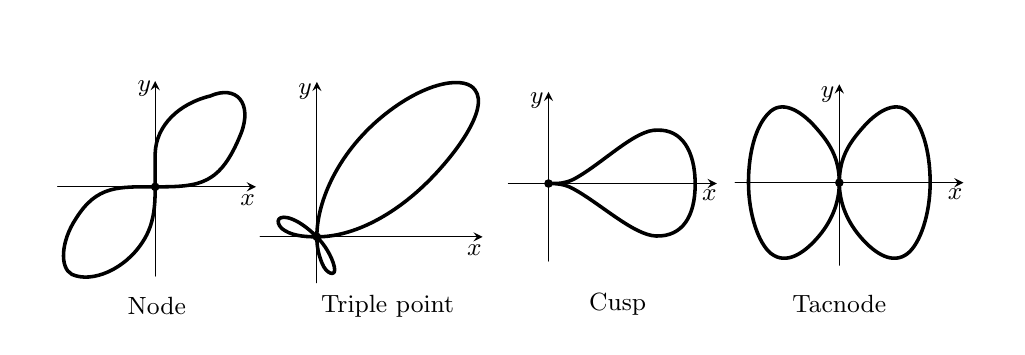
\begin{tikzpicture}[
    x=.3bp, y=-.3bp, line cap=round, line join=round, >=stealth,
    axis/.style={->,line width=.47bp},
    curve/.style={line width=1.28bp},
    every node/.style={inner sep=0pt,font=\small}
  ]
  \path[use as bounding box] (-24,-48) rectangle (1139.333,311.333);

  % At the node the two tangent lines are the coordinate axes.
  \coordinate (node) at (129,143);
  \draw[axis] (12,143) -- (250,143);
  \draw[axis] (129,250) -- (129,16);
  \draw[curve] (node)
    .. controls (183,143) and (207,141) .. (232,79)
    .. controls (246,43) and (227,20) .. (195,34)
    .. controls (158,43) and (130,69) .. (129,103)
    -- (node)
    .. controls (85,143) and (59,141) .. (34,181)
    .. controls (16,208) and (14,240) .. (29,248)
    .. controls (53,259) and (93,242) .. (114,209)
    .. controls (128,188) and (129,165) .. (node);
  \fill (node) circle[radius=1.55bp];
  \node at (116,25) {$y$};
  \node at (240,159) {$x$};
  \node at (131,286) {Node};

  % One lobe between each pair of adjacent tangents.
  \coordinate (triple) at (323,203);
  \draw[axis] (255,203) -- (522,203);
  \draw[axis] (323,258) -- (323,17);
  \draw[curve] (triple)
    .. controls (323,159) and (350,99) .. (406,55)
    .. controls (457,15) and (502,10) .. (513,27)
    .. controls (530,50) and (488,106) .. (454,139)
    .. controls (416,176) and (368,203) .. (triple);
  \draw[curve] (triple)
    .. controls (305,203) and (291,201) .. (281,193)
    .. controls (272,184) and (277,175) .. (294,182)
    .. controls (304,186) and (315,195) .. (triple)
    .. controls (332,212) and (341,226) .. (344,239)
    .. controls (347,252) and (334,248) .. (329,234)
    .. controls (325,224) and (323,215) .. (triple);
  \fill (triple) circle[radius=1.55bp];
  \node at (309,29) {$y$};
  \node at (512,219) {$x$};
  \node at (408,286) {Triple point};

  % The two halves of the cusp leave the origin along the positive x-axis.
  \coordinate (cusp) at (601,139);
  \draw[axis] (553,139) -- (803,139);
  \draw[axis] (601,232) -- (601,29);
  \draw[curve] (cusp)
    .. controls (615,139) and (620,139) .. (631,134)
    .. controls (665,116) and (706,73) .. (732,75)
    .. controls (761,74) and (777,100) .. (777,140)
    .. controls (777,178) and (762,203) .. (730,202)
    .. controls (703,201) and (662,162) .. (630,145)
    .. controls (621,140) and (612,139) .. (cusp);
  \fill (cusp) circle[radius=1.55bp];
  \node at (587,39) {$y$};
  \node at (794,153) {$x$};
  \node at (684,284) {Cusp};

  % The two lobes are both tangent to the vertical axis at the origin.
  \coordinate (tacnode) at (950,138);
  \draw[axis] (825,138) -- (1099,138);
  \draw[axis] (950,237) -- (950,20);
  \foreach \side in {-1,1} {
    \begin{scope}[shift={(tacnode)},xscale=\side]
      \draw[curve] (0,0)
        .. controls (0,-30) and (12,-48) .. (29,-67)
        .. controls (44,-84) and (66,-99) .. (82,-86)
        .. controls (99,-72) and (109,-39) .. (109,0)
        .. controls (109,38) and (97,73) .. (82,85)
        .. controls (64,99) and (43,85) .. (27,67)
        .. controls (10,48) and (0,25) .. (0,0);
    \end{scope}
  }
  \fill (tacnode) circle[radius=1.55bp];
  \node at (936,32) {$y$};
  \node at (1089,152) {$x$};
  \node at (950,284) {Tacnode};
\end{tikzpicture}
}\par
\noindent\makebox[\linewidth][c]{\small\textbf{Figure 4.}\quad Singularities of plane curves.}\par

\smallskip
\noindent\hypertarget{ex-I-5.2}{}\textbf{5.2.} Locate the singular points and describe the singularities of the following surfaces in $\AffSpace{3}$ (assume $\operatorname{char}k\ne2$). Which is which in Figure~\Goto{fig-book-5}{5}?
\begin{enumerate}[label=(\alph*),leftmargin=2.4em,nosep]
\item $xy^2=z^2$;
\item $x^2+y^2=z^2$;
\item $xy+x^3+y^3=0$.
\end{enumerate}

\noindent\hypertarget{fig-book-5}{}\resizebox{\linewidth}{!}{% Figure 5. Surface singularities (printed page 36).
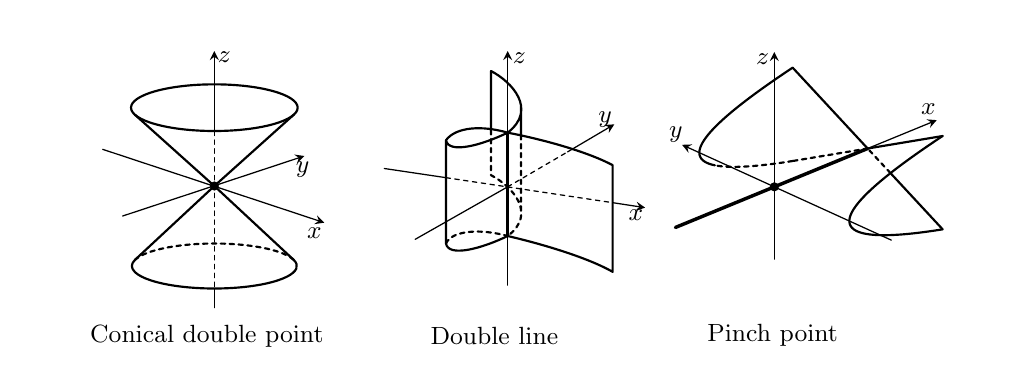
\begin{tikzpicture}[
    x=.3bp, y=-.3bp, line cap=round, line join=round, >=stealth,
    axis/.style={line width=.45bp},
    edge/.style={line width=.78bp},
    singular/.style={line width=1.24bp},
    hidden/.style={dash pattern=on 1.6bp off 1.6bp},
    every node/.style={inner sep=0pt,font=\small}
  ]
  \path[use as bounding box] (-34,-15) rectangle (1129.333,378.333);

  % Conical double point. The far rim of the lower cone is occluded.
  \coordinate (vertex) at (190,175);
  \draw[axis,->] (56,131) -- (322,219);
  \draw[axis,->] (80,211) -- (298,139);
  \draw[axis,->] (190,109) -- (190,13);
  \draw[axis,hidden] (190,109) -- (190,298);
  \draw[axis] (190,298) -- (190,321);
  \draw[edge] (190,81) ellipse[x radius=100, y radius=28];
  \draw[edge]
    (94.54,89.34) -- (vertex) -- (285.46,89.34)
    (95,263.41) -- (vertex) -- (285,263.41);
  \draw[edge,hidden] (285,263.41)
    arc[start angle=-16.33,end angle=-163.67,x radius=99,y radius=27];
  \draw[edge] (285,263.41)
    arc[start angle=-16.33,end angle=196.33,x radius=99,y radius=27];
  \fill (vertex) circle[radius=1.65bp];
  \node at (202,20) {$z$};
  \node at (296,155) {$y$};
  \node at (310,231) {$x$};
  \node at (181,355) {Conical double point};

  % Double line. The two sheets are drawn as vertical extrusions.
  \draw[axis] (394,154) -- (468,165);
  \draw[axis,hidden] (468,165) -- (668,195);
  \draw[axis,->] (668,195) -- (707,201);
  \draw[axis] (431,239) -- (542,176);
  \draw[axis,hidden] (542,176) -- (614,134);
  \draw[axis,->] (614,134) -- (670,101);
  \draw[axis,->] (542,294) -- (542,13);

  \draw[edge,hidden]
    (522,108) -- (522,162)
      .. controls (547,175) and (578,208) .. (542,235)
    (558,114) -- (558,207)
    (468,244) .. controls (475,228) and (510,226) .. (542,235);
  \draw[edge]
    (522,108) -- (522,37)
      .. controls (547,50) and (578,83) .. (542,111)
    (558,79) -- (558,114)
    (542,111) .. controls (589,120) and (640,135) .. (668,150)
      -- (668,278) .. controls (640,262) and (589,246) .. (542,235)
    (542,111) .. controls (511,102) and (480,104) .. (468,120)
      .. controls (471,137) and (511,126) .. (542,111)
    (468,120) -- (468,244)
      .. controls (471,261) and (511,250) .. (542,235);
  \draw[singular] (542,111) -- (542,235);
  \node at (556,21) {$z$};
  \node at (659,95) {$y$};
  \node at (696,210) {$x$};
  \node at (526,355) {Double line};

  % Pinch point. Orthographic projection of (x,y,z)=(s^2,t,st),
  % restricted to |s|,|t|<=1. Smaller x is closer in this view.
  \coordinate (pinch) at (862,176);
  \begin{scope}[
      shift={(pinch)},
      x={(33.6bp,13.8bp)}, y={(-27bp,12.3bp)}, z={(0bp,16.8bp)}
    ]
    \draw[axis,->] (0,-1.56,0) -- (0,1.23,0);
    \draw[axis,->] (0,0,-1.55) -- (0,0,2.89);
    \draw[axis,->] (1,0,0) -- (1.74,0,0);

    % The hidden part of the rim t=1, and the occluded ends at x=1.
    \draw[edge,hidden]
      plot[domain=-1:-.408,samples=24,variable=\s,smooth] ({\s*\s},1,{\s})
      (1,0,0) -- (1,1,-1)
      (1,-.304,-.304) -- (1,0,0);
    \draw[edge]
      plot[domain=-.408:1,samples=32,variable=\s,smooth] ({\s*\s},1,{\s});
    \draw[edge]
      plot[domain=-1:1,samples=42,variable=\s,smooth] ({\s*\s},-1,{-\s});
    \draw[edge]
      (1,-1,1) -- (1,0,0) -- (1,1,1)
      (1,-1,-1) -- (1,-.304,-.304);
    \draw[singular] (-1.06,0,0) -- (1,0,0);
    \fill (0,0,0) circle[radius=1.65bp];
  \end{scope}
  \node at (848,23) {$z$};
  \node at (744,113) {$y$};
  \node at (1047,83) {$x$};
  \node at (860,354) {Pinch point};
\end{tikzpicture}
}\par
\noindent\makebox[\linewidth][c]{\small\textbf{Figure 5.}\quad Surface singularities.}\par

\smallskip
\noindent\hypertarget{ex-I-5.3}{}\hypertarget{err-I-5-3-ex}{}\textbf{5.3.} \emph{Multiplicities.} Let $Y\subseteq\AffSpace{2}$ be a curve defined by the equation $f(x,y)=0$. Let $P=(a,b)$ be a point of $\AffSpace{2}$. \EditionText{Translate the coordinates so that $P$ becomes the point $(0,0)$.} Then write $f$ as a sum $f=f_0+f_1+\cdots+f_d$, where $f_i$ is a homogeneous polynomial of degree $i$ in $x$ and $y$. Then we define the \emph{multiplicity of $P$ on $Y$}, denoted $\mu_P(Y)$, to be the least $r$ such that $f_r\ne0$. (Note that $P\in Y\iff\mu_P(Y)>0$.) The linear factors of $f_r$ are called the \emph{tangent directions at $P$}.
\begin{enumerate}[label=(\alph*),leftmargin=2.4em,nosep]
\item Show that $\mu_P(Y)=1\iff P$ is a nonsingular point of $Y$.
\item Find the multiplicity of each of the singular points in (Ex. \Goto{ex-I-5.1}{5.1}) above.
\end{enumerate}

\smallskip
\noindent\hypertarget{ex-I-5.4}{}\textbf{5.4.} \emph{Intersection Multiplicity.} If $Y,Z\subseteq\AffSpace{2}$ are two distinct curves, given by equations $f=0$, $g=0$, and if $P\in Y\cap Z$, we define the \emph{intersection multiplicity} $(Y\cdot Z)_P$ of $Y$ and $Z$ at $P$ to be the length of the $\mathcal O_P$-module $\mathcal O_P/(f,g)$.
\begin{enumerate}[label=(\alph*),leftmargin=2.4em,nosep]
\item Show that $(Y\cdot Z)_P$ is finite, and $(Y\cdot Z)_P\ge\mu_P(Y)\cdot\mu_P(Z)$.
\item If $P\in Y$, show that for almost all lines $L$ through $P$ (i.e., all but a finite number), $(L\cdot Y)_P=\mu_P(Y)$.
\item If $Y$ is a curve of degree $d$ in $\Proj^2$, and if $L$ is a line in $\Proj^2$, $L\ne Y$, show that $(L\cdot Y)=d$. Here we define $(L\cdot Y)=\sum(L\cdot Y)_P$ taken over all points $P\in L\cap Y$, where $(L\cdot Y)_P$ is defined using a suitable affine cover of $\Proj^2$.
\end{enumerate}}
% Contents from body/page-051.tex.
\ChapterSheet[10.2]{51}{37}{\Goto{sec-I-5}{5\quad Nonsingular Varieties}}{%
\fontsize{9.6}{10.3}\selectfont\setlength{\parskip}{0pt}\setlength{\smallskipamount}{1pt}\noindent\hypertarget{ex-I-5.5}{}\textbf{5.5.} For every degree $d>0$, and every $p=0$ or a prime number, give the equation of a nonsingular curve of degree $d$ in $\Proj^2$ over a field $k$ of characteristic $p$.

\smallskip
\noindent\hypertarget{ex-I-5.6}{}\textbf{5.6.} \emph{Blowing Up Curve Singularities.}
\begin{enumerate}[label=(\alph*),leftmargin=2.4em,nosep]
\item \hypertarget{err-I-5-6a}{}Let $Y$ be the cusp or node of (Ex. \Goto{ex-I-5.1}{5.1}). Show that the curve $\widetilde Y$ obtained by blowing up $Y$ at $O=(0,0)$ is nonsingular\EditionText{ at every point over $O$} (cf. \Goto{result-I-4.9.1}{(4.9.1)} and Ex. \Goto{ex-I-4.10}{4.10}).
\item We define a \emph{node} (also called \emph{ordinary double point}) to be a double point (i.e., a point of multiplicity 2) of a plane curve with distinct tangent directions (Ex. \Goto{ex-I-5.3}{5.3}). If $P$ is a node on a plane curve $Y$, show that $\varphi^{-1}(P)$ consists of two distinct nonsingular points on the blown-up curve $\widetilde Y$. We say that \textquotedblleft{}blowing up $P$ resolves the singularity at $P$\textquotedblright{}.
\item Let $P\in Y$ be the tacnode of (Ex. \Goto{ex-I-5.1}{5.1}). If $\varphi\colon\widetilde Y\to Y$ is the blowing-up at $P$, show that $\varphi^{-1}(P)$ is a node. Using (b) we see that the tacnode can be resolved by two successive blowings-up.
\item Let $Y$ be the plane curve $y^3=x^5$, which has a \textquotedblleft{}higher order cusp\textquotedblright{} at $O$. Show that $O$ is a triple point; that blowing up $O$ gives rise to a double point (what kind?) and that one further blowing up resolves the singularity.
\end{enumerate}
\noindent\emph{Note:} We will see later \Goto{result-V-3.8}{(V, 3.8)} that any singular point of a plane curve can be resolved by a finite sequence of successive blowings-up.

\smallskip
\noindent\hypertarget{ex-I-5.7}{}\textbf{5.7.} Let $Y\subseteq\Proj^2$ be a nonsingular plane curve of degree $>1$, defined by the equation $f(x,y,z)=0$. Let $X\subseteq\AffSpace{3}$ be the affine variety defined by $f$ (this is the cone over $Y$; see (Ex. \Goto{ex-I-2.10}{2.10})). Let $P$ be the point $(0,0,0)$, which is the \emph{vertex} of the cone. Let $\varphi\colon\widetilde X\to X$ be the blowing-up of $X$ at $P$.
\begin{enumerate}[label=(\alph*),leftmargin=2.4em,nosep]
\item Show that $X$ has just one singular point, namely $P$.
\item Show that $\widetilde X$ is nonsingular (cover it with open affines).
\item Show that $\varphi^{-1}(P)$ is isomorphic to $Y$.
\end{enumerate}

\smallskip
\noindent\hypertarget{ex-I-5.8}{}\textbf{5.8.} Let $Y\subseteq\Proj^n$ be a projective variety of dimension $r$. Let $f_1,\ldots,f_t\in S=k[x_0,\ldots,x_n]$ be homogeneous polynomials which generate the ideal of $Y$. Let $P\in Y$ be a point, with homogeneous coordinates $P=(a_0,\ldots,a_n)$. Show that $P$ is nonsingular on $Y$ if and only if the rank of the matrix $\lVert(\partial f_i/\partial x_j)(a_0,\ldots,a_n)\rVert$ is $n-r$. [\emph{Hint:} (a) Show that this rank is independent of the homogeneous coordinates chosen for $P$; (b) pass to an open affine $U_i\subseteq\Proj^n$ containing $P$ and use the affine Jacobian matrix; (c) you will need Euler's lemma, which says that if $f$ is a homogeneous polynomial of degree $d$, then $\sum x_i(\partial f/\partial x_i)=d\cdot f$.]

\smallskip
\noindent\hypertarget{ex-I-5.9}{}\hypertarget{err-I-5-9}{}\textbf{5.9.} Let $f\in k[x,y,z]$ be a homogeneous polynomial\EditionText{ of positive degree}, let $Y=Z(f)\subseteq\Proj^2$ be the algebraic set defined by $f$, and suppose that for every $P\in Y$, at least one of $(\partial f/\partial x)(P)$, $(\partial f/\partial y)(P)$, $(\partial f/\partial z)(P)$ is nonzero. Show that $f$ is irreducible (and hence that $Y$ is a nonsingular variety). [\emph{Hint:} Use (Ex. \Goto{ex-I-3.7}{3.7}).]

\smallskip
\noindent\hypertarget{ex-I-5.10}{}\textbf{5.10.} For a point $P$ on a variety $X$, let $\mathfrak m$ be the maximal ideal of the local ring $\mathcal O_P$. We define the \emph{Zariski tangent space} $T_P(X)$ of $X$ at $P$ to be the dual $k$-vector space of $\mathfrak m/\mathfrak m^2$.
\begin{enumerate}[label=(\alph*),leftmargin=2.4em,nosep]
\item For any point $P\in X$, $\dim T_P(X)\ge\dim X$, with equality if and only if $P$ is nonsingular.
\item For any morphism $\varphi\colon X\to Y$, there is a natural induced $k$-linear map $T_P(\varphi)\colon T_P(X)\to T_{\varphi(P)}(Y)$.
\item If $\varphi$ is the vertical projection of the parabola $x=y^2$ onto the $x$-axis, show that the induced map $T_0(\varphi)$ of tangent spaces at the origin is the zero map.
\end{enumerate}}
% Contents from body/page-052.tex.
\ChapterSheet[10.5]{52}{38}{\Goto{p-15}{I\quad Varieties}}{%
\setlength{\parskip}{0pt}\noindent\hypertarget{ex-I-5.11}{}\hypertarget{err-I-5-11}{}\textbf{5.11.} \emph{The Elliptic Quartic Curve in $\Proj^3$.} \EditionText{Assume $\operatorname{char}k\ne2$. }Let $Y$ be the algebraic set in $\Proj^3$ defined by the equations $x^2-xz-yw=0$ and $yz-xw-zw=0$. Let $P$ be the point $(x,y,z,w)=(0,0,0,1)$, and let $\varphi$ denote the projection from $P$ to the plane $w=0$. Show that $\varphi$ induces an isomorphism of $Y-P$ with the plane cubic curve $y^2z-x^3+xz^2=0$ minus the point $(1,0,-1)$. Then show that $Y$ is an irreducible nonsingular curve. It is called the \emph{elliptic quartic curve} in $\Proj^3$. Since it is defined by two equations it is another example of a complete intersection (Ex. \Goto{ex-I-2.17}{2.17}).

\smallskip
\noindent\hypertarget{ex-I-5.12}{}\textbf{5.12.} \emph{Quadric Hypersurfaces.} Assume $\operatorname{char}k\ne2$, and let $f$ be a homogeneous polynomial of degree $2$ in $x_0,\ldots,x_n$.
\begin{enumerate}[label=(\alph*),leftmargin=2.4em,nosep]
\item Show that after a suitable linear change of variables, $f$ can be brought into the form $f=x_0^2+\cdots+x_r^2$ for some $0\le r\le n$.
\item Show that $f$ is irreducible if and only if $r\ge2$.
\item Assume $r\ge2$, and let $Q$ be the quadric hypersurface in $\Proj^n$ defined by $f$. \hypertarget{err-I-5-12c}{}\EditionText{Show that the singular locus $Z=\operatorname{Sing}Q$ is empty if $r=n$, and otherwise is a linear variety (Ex. \Goto{ex-I-2.11}{2.11}) of dimension $n-r-1$.} In particular, $Q$ is nonsingular if and only if $r=n$.
\item In case $r<n$, show that $Q$ is a \emph{cone with axis $Z$} over a nonsingular quadric hypersurface $Q'\subseteq\Proj^r$. (This notion of cone generalizes the one defined in (Ex. \Goto{ex-I-2.10}{2.10}). If $Y$ is a closed subset of $\Proj^r$, and if $Z$ is a linear subspace of dimension $n-r-1$ in $\Proj^n$, we embed $\Proj^r$ in $\Proj^n$ so that $\Proj^r\cap Z=\varnothing$, and define the \emph{cone over $Y$ with axis $Z$} to be the union of all lines joining a point of $Y$ to a point of $Z$.)
\end{enumerate}

\smallskip
\noindent\hypertarget{ex-I-5.13}{}\textbf{5.13.} It is a fact that any regular local ring is an integrally closed domain (Matsumura \Goto{legacy-b-mat}{[2, Th. 36, p. 121]}). Thus we see from \Goto{result-I-5.3}{(5.3)} that any variety has a nonempty open subset of normal points (Ex. \Goto{ex-I-3.17}{3.17}). In this exercise, show directly (without using \Goto{result-I-5.3}{(5.3)}) that the set of nonnormal points of a variety is a proper closed subset (you will need the finiteness of integral closure: see \Goto{result-I-3.9A}{(3.9A)}).

\smallskip
\noindent\hypertarget{ex-I-5.14}{}\textbf{5.14.} \emph{Analytically Isomorphic Singularities.}
\begin{enumerate}[label=(\alph*),leftmargin=2.4em,nosep]
\item If $P\in Y$ and $Q\in Z$ are analytically isomorphic \emph{plane curve} singularities, show that the multiplicities $\mu_P(Y)$ and $\mu_Q(Z)$ are the same (Ex. \Goto{ex-I-5.3}{5.3}).
\item Generalize the example in the text \Goto{result-I-5.6.3}{(5.6.3)} to show that if $f=f_r+f_{r+1}+\cdots\in k[[x,y]]$, and if the leading form $f_r$ of $f$ factors as $f_r=g_s h_t$, where $g_s,h_t$ are homogeneous of degrees $s$ and $t$ respectively, and have no common linear factor, then there are formal power series
\[
\begin{aligned}
g&=g_s+g_{s+1}+\cdots\\
h&=h_t+h_{t+1}+\cdots
\end{aligned}
\]
in $k[[x,y]]$ such that $f=gh$.
\item Let $Y$ be defined by the equation $f(x,y)=0$ in $\AffSpace{2}$, and let $P=(0,0)$ be a point of multiplicity $r$ on $Y$, so that when $f$ is expanded as a polynomial in $x$ and $y$, we have $f=f_r+\text{higher terms}$. We say that $P$ is an \emph{ordinary $r$-fold point} if $f_r$ is a product of $r$ \emph{distinct} linear factors. Show that any two ordinary double points are analytically isomorphic. Ditto for ordinary triple points. But show that there is a one-parameter family of mutually nonisomorphic ordinary 4-fold points.
\item[*(d)] Assume $\operatorname{char}k\ne2$. Show that any double point of a plane curve is analytically isomorphic to the singularity at $(0,0)$ of the curve $y^2=x^r$, for a uniquely
\end{enumerate}}
% Contents from body/page-053.tex.
\BookMark{1}{1.6  Nonsingular Curves}{sec-I-6}
\ChapterSheet{53}{39}{\Goto{sec-I-6}{6\quad Nonsingular Curves}}{%
\noindent\hangindent=2.4em\hangafter=0\hspace*{2.4em}determined $r\ge2$. If $r=2$ it is a node (Ex. \Goto{ex-I-5.6}{5.6}). If $r=3$ we call it a \emph{cusp}; if $r=4$ a \emph{tacnode}. See \Goto{result-V-3.9.5}{(V, 3.9.5)} for further discussion.\par

\smallskip
\noindent\hypertarget{ex-I-5.15}{}\textbf{5.15.} \emph{Families of Plane Curves.} A homogeneous polynomial $f$ of \EditionText{positive }degree $d$ in three variables $x,y,z$ has $\binom{d+2}{2}$ coefficients. Let these coefficients represent a point in $\Proj^N$, where $N=\binom{d+2}{2}-1=\tfrac12d(d+3)$.
\begin{enumerate}[label=(\alph*),leftmargin=2.4em,nosep]
\item Show that this gives a correspondence between points of $\Proj^N$ and algebraic sets in $\Proj^2$ which can be defined by an equation of degree $d$. The correspondence is 1-1 except in some cases where $f$ has a multiple factor.
\item Show under this correspondence that the (irreducible) nonsingular curves of degree $d$ correspond 1-1 to the points of a nonempty Zariski-open subset of $\Proj^N$. [\emph{Hints:} (1) \hypertarget{err-I-5-15b}{}Use elimination theory \Goto{result-I-5.7A}{(5.7A)} applied to the homogeneous polynomials \EditionText{$f,\partial f/\partial x,\partial f/\partial y,\partial f/\partial z$}; (2) use the previous (Ex. \Goto{ex-I-5.5}{5.5}, \Goto{ex-I-5.8}{5.8}, \Goto{ex-I-5.9}{5.9}) above.]
\end{enumerate}

\bigskip
\noindent\hypertarget{sec-I-6}{}\textbf{\large 6\quad Nonsingular Curves}\par
\smallskip
\noindent In considering the problem of classification of algebraic varieties, we can formulate several subproblems, based on the idea that a nonsingular projective variety is the best kind: (a) classify varieties up to birational equivalence; (b) within each birational equivalence class, find a nonsingular projective variety; (c) classify the nonsingular projective varieties in a given birational equivalence class.

In general, all three problems are very difficult. However, in the case of curves, the situation is much simpler. In this section we will answer problems (b) and (c) by showing that in each birational equivalence class, there is a unique nonsingular projective curve. We will also give an example to show that not all curves are birationally equivalent to each other (Ex. \Goto{ex-I-6.2}{6.2}). Thus for a given finitely generated extension field $K$ of $k$ of transcendence degree $1$ (which we will call a \emph{function field of dimension 1}) we can talk about the nonsingular projective curve $C_K$ with function field equal to $K$. We will see also that if $K_1,K_2$ are two function fields of dimension $1$, then any $k$-homomorphism $K_2\to K_1$ is represented by a morphism of $C_{K_1}$ to $C_{K_2}$.

We will begin our study in an oblique manner by defining the notion of an \textquotedblleft{}abstract nonsingular curve\textquotedblright{} associated with a given function field. It will not be clear a priori that this is a variety. However, we will see in retrospect that we have defined nothing new.

First we have to recall some basic facts about valuation rings and Dedekind domains.

\smallskip
\noindent\hypertarget{err-I-6-valuation}{}\textbf{Definition.} Let $K$ be a field and let $G$ be a totally ordered abelian group. A \emph{valuation of $K$ with values in $G$} is a map $v\colon K-\{0\}\to G$ such that for all $x,y\in K$, $x,y\ne0$, we have \EditionText{(with the convention $v(0)=+\infty$)}:
\begin{enumerate}[label=(\arabic*),leftmargin=2.4em,nosep]
\item $v(xy)=v(x)+v(y)$;
\item $v(x+y)\ge\min(v(x),v(y))$.
\end{enumerate}}
% Contents from body/page-054.tex.
\ChapterSheet{54}{40}{\Goto{p-15}{I\quad Varieties}}{%
\noindent If $v$ is a valuation, then the set $R=\{x\in K\mid v(x)\ge0\}\cup\{0\}$ is a subring of $K$, which we call the \emph{valuation ring} of $v$. The subset $\mathfrak m=\{x\in K\mid v(x)>0\}\cup\{0\}$ is an ideal in $R$, and $R,\mathfrak m$ is a local ring. A \emph{valuation ring} is an integral domain which is the valuation ring of some valuation of its quotient field. If $R$ is a valuation ring with quotient field $K$, we say that $R$ is a valuation ring of $K$. If $k$ is a subfield of $K$ such that $v(x)=0$ for all $x\in k-\{0\}$, then we say $v$ is a valuation of $K/k$, and $R$ is a valuation ring of $K/k$. (Note that valuation rings are not in general noetherian!)

\smallskip
\noindent\textbf{Definition.} If $A,B$ are local rings contained in a field $K$, we say that $B$ \emph{dominates} $A$ if $A\subseteq B$ and $\mathfrak m_B\cap A=\mathfrak m_A$.

\smallskip
\noindent\hypertarget{result-I-6.1A}{}\textbf{Theorem 6.1A.} \emph{Let $K$ be a field. A local ring $R$ contained in $K$ is a valuation ring of $K$ if and only if it is a maximal element of the set of local rings contained in $K$, with respect to the relation of domination. Every local ring contained in $K$ is dominated by some valuation ring of $K$.}

\smallskip
\noindent\textsc{Proof.} Bourbaki \hypertarget{err-I-6-1A-bourbaki}{}\EditionText{\Goto{bib-474-4-item-1}{[1, Ch. VI, \S1, no.~2, Ths.~1--2 and corollary]}} or Atiyah--Macdonald \Goto{legacy-b-am}{[1, Ch. 5, p. 65, and exercises, p. 72]}.

\smallskip
\noindent\hypertarget{err-I-6-discrete}{}\textbf{Definition.} A valuation $v$ is \emph{discrete} if its \EditionText{value group $v(K\setminus\{0\})$ is order-isomorphic to the integers}. The corresponding valuation ring is called a \emph{discrete valuation ring}.

\smallskip
\noindent\hypertarget{result-I-6.2A}{}\textbf{Theorem 6.2A.} \emph{Let $A$ be a noetherian local domain of dimension one, with maximal ideal $\mathfrak m$. Then the following conditions are equivalent:}
\begin{enumerate}[label=(\roman*),leftmargin=2.4em,nosep]
\itshape
\item $A$ is a discrete valuation ring;
\item $A$ is integrally closed;
\item $A$ is a regular local ring;
\item $\mathfrak m$ is a principal ideal.
\end{enumerate}

\smallskip
\noindent\textsc{Proof.} Atiyah--Macdonald \Goto{legacy-b-am}{[1, Prop. 9.2, p. 94]}.

\smallskip
\noindent\textbf{Definition.} A \emph{Dedekind domain} is an integrally closed noetherian domain of dimension one.

\smallskip
Because integral closure is a local property (Atiyah--Macdonald \Goto{legacy-b-am}{[1, Prop. 5.13, p. 63]}), every localization of a Dedekind domain at a nonzero prime ideal is a discrete valuation ring.

\smallskip
\noindent\hypertarget{result-I-6.3A}{}\textbf{Theorem 6.3A.} \emph{The integral closure of a Dedekind domain in a finite extension field of its quotient field is again a Dedekind domain.}

\smallskip
\noindent\textsc{Proof.} Zariski--Samuel \Goto{legacy-b-zs}{[1, vol. 1, Th. 19, p. 281]}.

\smallskip
We now turn to the case of a function field $K$ of dimension $1$ over $k$, where $k$ is our fixed algebraically closed base field. We wish to establish a connection}
% Contents from body/page-055.tex.
\ChapterSheet{55}{41}{\Goto{sec-I-6}{6\quad Nonsingular Curves}}{%
\noindent between nonsingular curves with function field $K$ and the set of discrete valuation rings of $K/k$. If $P$ is a point on a nonsingular curve $Y$, then by \Goto{result-I-5.1}{(5.1)} the local ring $\mathcal O_P$ is a regular local ring of dimension one, and so by \Goto{result-I-6.2A}{(6.2A)} it is a discrete valuation ring. Its quotient field is the function field $K$ of $Y$, and since $k\subseteq\mathcal O_P$, it is a valuation ring of $K/k$. Thus the local rings of $Y$ define a subset of the set $C_K$ of all discrete valuation rings of $K/k$. This motivates the definition of an abstract nonsingular curve below. But first we need a few more preliminaries.

\smallskip
\noindent\hypertarget{result-I-6.4}{}\textbf{Lemma 6.4.} \emph{Let $Y$ be a quasi-projective variety, let $P,Q\in Y$, and suppose that $\mathcal O_Q\subseteq\mathcal O_P$ as subrings of $K(Y)$. Then $P=Q$.}

\smallskip
\noindent\textsc{Proof.} Embed $Y$ in $\Proj^n$ for some $n$. Replacing $Y$ by its closure, we may assume $Y$ is projective. After a suitable linear change of coordinates in $\Proj^n$, we may assume that neither $P$ nor $Q$ is in the hyperplane $H_0$ defined by $x_0=0$. Thus $P,Q\in Y\cap(\Proj^n-H_0)$ which is affine, so we may assume that $Y$ is an affine variety.

Let $A$ be the affine ring of $Y$. Then there are maximal ideals $\mathfrak m,\mathfrak n\subseteq A$ such that $\mathcal O_P=A_{\mathfrak m}$ and $\mathcal O_Q=A_{\mathfrak n}$. If $\mathcal O_Q\subseteq\mathcal O_P$, we must have $\mathfrak m\subseteq\mathfrak n$. But $\mathfrak m$ is a maximal ideal, so $\mathfrak m=\mathfrak n$, hence $P=Q$, by \Goto{result-I-3.2}{(3.2b)}.

\smallskip
\noindent\hypertarget{result-I-6.5}{}\textbf{Lemma 6.5.} \emph{Let $K$ be a function field of dimension one over $k$, and let $x\in K$. Then $\{R\in C_K\mid x\notin R\}$ is a finite set.}

\smallskip
\noindent\textsc{Proof.} \EditionText{The claim is immediate for $x=0$. Suppose $x\ne0$. }If $R$ is a valuation ring, then $x\notin R$ if and only if $1/x\in\mathfrak m_R$. So letting $y=1/x$, we have to show that if $y\in K$, $y\ne0$, then $\{R\in C_K\mid y\in\mathfrak m_R\}$ is a finite set. If $y\in k$, there are no such $R$, so let us assume $y\notin k$.

We consider the subring $k[y]$ of $K$ generated by $y$. Since $k$ is algebraically closed, $y$ is transcendental over $k$, hence $k[y]$ is a polynomial ring. Furthermore, since $K$ is finitely generated and of transcendence degree $1$ over $k$, $K$ is a finite field extension of $k(y)$. Now let $B$ be the integral closure of $k[y]$ in $K$. Then by \Goto{result-I-6.3A}{(6.3A)}, $B$ is a Dedekind domain, and it is also a finitely generated $k$-algebra \Goto{result-I-3.9A}{(3.9A)}.

Now if $y$ is contained in a discrete valuation ring $R$ of $K/k$, then $k[y]\subseteq R$, and since $R$ is integrally closed in $K$, we have $B\subseteq R$. \hypertarget{err-I-6-5}{}Let $\mathfrak n=\mathfrak m_R\cap B$. \EditionText{If $\mathfrak n=0$, then every nonzero element of $B$ is a unit in $R$, forcing $R=K$. Thus $\mathfrak n$ is a maximal ideal of $B$, and $B_{\mathfrak n}$ is dominated by $R$.} But $B_{\mathfrak n}$ is also a discrete valuation ring of $K/k$, hence $B_{\mathfrak n}=R$ by the maximality of valuation rings \Goto{result-I-6.1A}{(6.1A)}.

If furthermore $y\in\mathfrak m_R$, then $y\in\mathfrak n$. Now $B$ is the affine coordinate ring of some affine variety $Y$ \Goto{result-I-1.4.6}{(1.4.6)}. Since $B$ is a Dedekind domain, $Y$ has dimension one and is nonsingular. To say that $y\in\mathfrak n$ says that $y$, as a regular function on $Y$, vanishes at the point of $Y$ corresponding to $\mathfrak n$. But $y\ne0$, so it vanishes only at a finite set of points; these are in 1-1 correspondence with the maximal ideals of $B$ by \Goto{result-I-3.2}{(3.2)}, and $R=B_{\mathfrak n}$ is determined by the maximal ideal $\mathfrak n$. Hence we conclude that $y\in\mathfrak m_R$ for only finitely many $R\in C_K$, as required.}
% Contents from body/page-056.tex.
\ChapterSheet{56}{42}{\Goto{p-15}{I\quad Varieties}}{%
\noindent\hypertarget{result-I-6.6}{}\textbf{Corollary 6.6.} \emph{Any discrete valuation ring of $K/k$ is isomorphic to the local ring of a point on some nonsingular affine curve.}

\smallskip
\noindent\textsc{Proof.} Given $R$, let $y\in R-k$. Then the construction used in the proof of \Goto{result-I-6.5}{(6.5)} gives such a curve.

\medskip
We now come to the definition of an abstract nonsingular curve. Let $K$ be a function field of dimension $1$ over $k$ (i.e., a finitely generated extension field of transcendence degree $1$). Let $C_K$ be the set of all discrete valuation rings of $K/k$. We will sometimes call the elements of $C_K$ \emph{points}, and write $P\in C_K$, where $P$ stands for the valuation ring $R_P$. Note that the set $C_K$ is infinite, because it contains all the local rings of any nonsingular curve with function field $K$; those local rings are all distinct \Goto{result-I-6.4}{(6.4)}, and there are infinitely many of them (Ex. \Goto{ex-I-4.8}{4.8}). We make $C_K$ into a topological space by taking the closed sets to be the finite subsets and the whole space. If $U\subseteq C_K$ is a\EditionText{ nonempty} open subset of $C_K$, we define the \emph{ring of regular functions on $U$} to be $\mathcal O(U)=\bigcap_{P\in U}R_P$. An element $f\in\mathcal O(U)$ defines a function from $U$ to $k$ by taking $f(P)$ to be the residue of $f$ modulo the maximal ideal of $R_P$. (Note by \Goto{result-I-6.6}{(6.6)} that for any $R\in C_K$, the residue field of $R$ is $k$.) If two elements $f,g\in\mathcal O(U)$ define the same function, then $f-g\in\mathfrak m_P$ for infinitely many $P\in C_K$, so by \Goto{result-I-6.5}{(6.5)} and its proof, $f=g$. Thus we can identify the elements of $\mathcal O(U)$ with functions from $U$ to $k$. \EditionText{On the empty set take the zero ring, consisting of the empty function. }Note also by \Goto{result-I-6.5}{(6.5)} that any $f\in K$ is a regular function on some open set $U$. Thus the function field of $C_K$, defined as in \Goto{sec-I-3}{\S3}, is just $K$.

\medskip
\noindent\hypertarget{err-I-6-nonempty}{}\textbf{Definition.} An \emph{abstract nonsingular curve} is a\EditionText{ nonempty} open subset $U\subseteq C_K$, where $K$ is a function field of dimension $1$ over $k$, with the induced topology, and the induced notion of regular functions on its open subsets.

\medskip
Note that it is not clear a priori that such an abstract curve is a variety. So we will enlarge the category of varieties by adjoining the abstract curves:

\medskip
\noindent\textbf{Definition.} A \emph{morphism} $\varphi\colon X\to Y$ between abstract nonsingular curves or varieties is a continuous mapping such that for every open set $V\subseteq Y$, and every regular function $f\colon V\to k$, $f\circ\varphi$ is a regular function on $\varphi^{-1}(V)$.

\medskip
Now that we have apparently enlarged our category, our task will be to show that every nonsingular quasi-projective curve is isomorphic to an abstract nonsingular curve, and conversely. In particular, we will show that $C_K$ itself is isomorphic to a nonsingular projective curve.

\medskip
\noindent\hypertarget{result-I-6.7}{}\textbf{Proposition 6.7.} \emph{Every nonsingular quasi-projective curve $Y$ is isomorphic to an abstract nonsingular curve.}}
% Contents from body/page-057.tex.
\ChapterSheet{57}{43}{\Goto{sec-I-6}{6\quad Nonsingular Curves}}{%
\noindent\textsc{Proof.} Let $K$ be the function field of $Y$. Then each local ring $\mathcal O_P$ of a point $P\in Y$ is a discrete valuation ring of $K/k$, by \Goto{result-I-5.1}{(5.1)} and \Goto{result-I-6.2A}{(6.2A)}. Furthermore, by \Goto{result-I-6.4}{(6.4)}, distinct points give rise to distinct subrings of $K$. So let $U\subseteq C_K$ be the set of local rings of $Y$, and let $\varphi\colon Y\to U$ be the bijective map defined by $\varphi(P)=\mathcal O_P$.

First, we need to show that $U$ is an open subset of $C_K$. Because open sets are complements of finite sets, it is sufficient to show that $U$ contains a nonempty open set. Thus, by \Goto{result-I-4.3}{(4.3)}, we may assume $Y$ is affine, with affine ring $A$. Then $A$ is a finitely generated $k$-algebra, and by \Goto{result-I-3.2}{(3.2)}, $K$ is the quotient field of $A$, and $U$ is the set of localizations of $A$ at its maximal ideals. Since these local rings are all discrete valuation rings, $U$ consists in fact of all discrete valuation rings of $K/k$ containing $A$. Now let $x_1,\ldots,x_n$ be a set of generators of $A$ over $k$. Then $A\subseteq R_P$ if and only if $x_1,\ldots,x_n\in R_P$. Thus $U=\bigcap U_i$, where $U_i=\{P\in C_K\mid x_i\in R_P\}$. But by \Goto{result-I-6.5}{(6.5)}, $\{P\in C_K\mid x_i\notin R_P\}$ is a finite set. Therefore each $U_i$ and hence also $U$ is open.

So we have shown that the $U$ defined above is an abstract nonsingular curve. To show that $\varphi$ is an isomorphism, we need only check that the regular functions on any open set are the same. But this follows from the definition of the regular functions on $U$ and the fact that for \EditionText{any nonempty open set} $V\subseteq Y$, $\mathcal O(V)=\bigcap_{P\in V}\mathcal O_{P,Y}$.

\medskip
Now we need a result about extensions of morphisms from curves to projective varieties, which is interesting in its own right.

\medskip
\noindent\hypertarget{result-I-6.8}{}\textbf{Proposition 6.8.} \emph{Let $X$ be an abstract nonsingular curve, let $P\in X$, let $Y$ be a projective variety, and let $\varphi\colon X-P\to Y$ be a morphism. Then there exists a unique morphism $\overline\varphi\colon X\to Y$ extending $\varphi$.}

\smallskip
\noindent\textsc{Proof.} Embed $Y$ as a closed subset of $\Proj^n$ for some $n$. Then it will be sufficient to show that $\varphi$ extends to a morphism of $X$ into $\Proj^n$, because if it does, the image is necessarily contained in $Y$. Thus we reduce to the case $Y=\Proj^n$.

Let $\Proj^n$ have homogeneous coordinates $x_0,\ldots,x_n$, and let $U$ be the open set where $x_0,\ldots,x_n$ are all nonzero. By using induction on $n$, we may assume that $\varphi(X-P)\cap U\ne\varnothing$. Because if $\varphi(X-P)\cap U=\varnothing$, then $\varphi(X-P)\subseteq\Proj^n-U$. But $\Proj^n-U$ is the union of the hyperplanes $H_i$ defined by $x_i=0$. Since $\varphi(X-P)$ is irreducible, it must be contained in $H_i$ for some $i$. Now $H_i\cong\Proj^{n-1}$, so the result would follow by induction. So we will assume that $\varphi(X-P)\cap U\ne\varnothing$.

For each $i,j$, $x_i/x_j$ is a regular function on $U$. Pulling it back by $\varphi$, we obtain a regular function $f_{ij}$ on an open subset of $X$, which we view as a rational function on $X$, i.e., $f_{ij}\in K$, where $K$ is the function field of $X$.

Let $v$ be the valuation of $K$ associated with the valuation ring $R_P$. Let $r_i=v(f_{i0})$, $i=0,1,\ldots,n$, $r_i\in\mathbb Z$. Then since $x_i/x_j=(x_i/x_0)/(x_j/x_0)$, we have
\[
v(f_{ij})=r_i-r_j\qquad i,j=0,\ldots,n.
\]}
% Contents from body/page-058.tex.
\ChapterSheet{58}{44}{\Goto{p-15}{I\quad Varieties}}{%
\noindent Choose $k$ such that $r_k$ is minimal among $r_0,\ldots,r_n$. Then $v(f_{ik})\ge0$ for all $i$, hence $f_{0k},\ldots,f_{nk}\in R_P$. Now define $\overline\varphi(P)=(f_{0k}(P),\ldots,f_{nk}(P))$, and $\overline\varphi(Q)=\varphi(Q)$ for $Q\ne P$. I claim that $\overline\varphi$ is a morphism of $X$ to $\Proj^n$ which extends $\varphi$, and that $\overline\varphi$ is unique. \hypertarget{err-I-6-8}{}%
\EditionText{}%
\EditionText{To show that $\overline\varphi$ is a morphism near $P$, take a common open neighborhood $W$ of $P$ on which $f_{0k},\ldots,f_{nk}$ are regular. Since $f_{kk}=1$, these functions give a morphism from $W$ to the affine chart $U_k=\{x_k\ne0\}$, whose coordinate ring is
\[
k[x_0/x_k,\ldots,x_n/x_k].
\]
On $(W\setminus\{P\})\cap\varphi^{-1}(U_j)$, put $a_i=(x_i/x_j)\circ\varphi$. On each such nonempty open set, $a_i=a_k f_{ik}$ as rational functions, hence as regular functions. Taking $i=j$ gives $1=a_k f_{jk}$, so $\varphi$ lies in $U_k$ there and agrees with the constructed morphism. Thus it glues with $\varphi$, with regular pullbacks from $V$ defined on $\overline\varphi^{-1}(V)$. For uniqueness, an extension taking $P$ into $U_j$ makes every $f_{ij}$ regular at $P$, so $r_j$ is minimal. Then $f_{kj}$ is a unit at $P$, and the value in $U_k$ is the one prescribed by the $f_{ik}(P)$.}

\medskip
Now we come to our main result.

\medskip
\noindent\hypertarget{result-I-6.9}{}\textbf{Theorem 6.9.} \emph{Let $K$ be a function field of dimension $1$ over $k$. Then the abstract nonsingular curve $C_K$ defined above is isomorphic to a nonsingular projective curve.}

\smallskip
\noindent\textsc{Proof.} The idea of the proof is this: we first cover $C=C_K$ with open subsets $U_i$ which are isomorphic to nonsingular affine curves. Let $Y_i$ be the projective closure of this affine curve. Then we use \Goto{result-I-6.8}{(6.8)} to define a morphism $\varphi_i\colon C\to Y_i$. Next, we consider the product mapping $\varphi\colon C\to\prod Y_i$, and let $Y$ be the closure of the image of $C$. Then $Y$ is a projective curve, and we show that $\varphi$ is an isomorphism of $C$ onto $Y$.

To begin with, let $P\in C$ be any point. Then by \Goto{result-I-6.6}{(6.6)} there is a nonsingular affine curve $V$ and a point $Q\in V$ with $R_P\cong\mathcal O_Q$. It follows that the function field of $V$ is $K$, and then by \Goto{result-I-6.7}{(6.7)}, $V$ is isomorphic to an open subset of $C$. Thus we have shown that every point $P\in C$ has an open neighborhood which is isomorphic to an affine variety.

Since $C$ is quasi-compact, we can cover it with a finite number of open subsets $U_i$, each of which is isomorphic to an affine variety $V_i$. Embed $V_i\subseteq\AffSpace{n_i}$, think of $\AffSpace{n_i}$ as an open subset of $\Proj^{n_i}$, and let $Y_i$ be the closure of $V_i$ in $\Proj^{n_i}$. Then $Y_i$ is a projective variety, and we have a morphism $\varphi_i\colon U_i\to Y_i$ which is an isomorphism of $U_i$ onto its image.

By \Goto{result-I-6.8}{(6.8)} applied to the finite set of points $C-U_i$, we can find a morphism $\overline\varphi_i\colon C\to Y_i$ extending $\varphi_i$. Let $\prod Y_i$ be the product of the projective varieties $Y_i$ (Ex. \Goto{ex-I-3.16}{3.16}). Then $\prod Y_i$ is also a projective variety. Let $\varphi\colon C\to\prod Y_i$ be the \textquotedblleft{}diagonal\textquotedblright{} map $\varphi(P)=\prod\overline\varphi_i(P)$, and let $Y$ be the closure of the image of $\varphi$. Then $Y$ is a projective variety, and $\varphi\colon C\to Y$ is a morphism whose image is dense in $Y$. (It follows that $Y$ is a curve.)

Now we must show that $\varphi$ is an isomorphism. For any point $P\in C$, we have $P\in U_i$ for some $i$. There is a commutative diagram}
% Contents from body/page-059.tex.
\ChapterSheet{59}{45}{\Goto{sec-I-6}{6\quad Nonsingular Curves}}{%
\noindent\makebox[\linewidth][c]{%
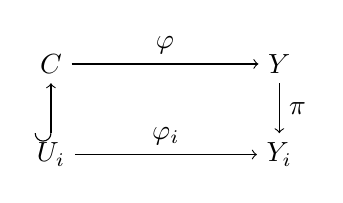
\begin{tikzpicture}[x=2.9cm,y=1.15cm,baseline=(current bounding box.center)]
  \node (C) at (0,1) {$C$};
  \node (Y) at (1,1) {$Y$};
  \node (U) at (0,0) {$U_i$};
  \node (Yi) at (1,0) {$Y_i$};
  \draw[->] (C)-- node[above] {$\varphi$} (Y);
  \draw[->] (U.north)--(C.south);
  \draw (U.north) arc[start angle=0,end angle=-180,radius=1mm];
  \draw[->] (U)-- node[above] {$\varphi_i$} (Yi);
  \draw[->] (Y)-- node[right] {$\pi$} (Yi);
\end{tikzpicture}}\par
\smallskip
\noindent of dominant morphisms, where $\pi$ is the projection map onto the $i$th factor. Thus we have inclusions of local rings
\[
\mathcal O_{\varphi_i(P),Y_i}\hookrightarrow\mathcal O_{\varphi(P),Y}\hookrightarrow\mathcal O_{P,C}
\]
by (Ex. \Goto{ex-I-3.3}{3.3}). The two outside ones are isomorphic, so the middle one is also. Thus we see that for any $P\in C$, the map $\varphi_P^*\colon\mathcal O_{\varphi(P),Y}\to\mathcal O_{P,C}$ is an isomorphism.

Next, let $Q$ be any point of $Y$. Then $\mathcal O_Q$ is dominated by some discrete valuation ring $R$ of $K/k$ (take for example a localization of the integral closure of $\mathcal O_Q$ at a maximal ideal). But $R=R_P$ for some $P\in C$, and $\mathcal O_{\varphi(P)}\cong R$, so by \Goto{result-I-6.4}{(6.4)} we must have $Q=\varphi(P)$. This shows that $\varphi$ is surjective. But $\varphi$ is clearly injective, because distinct points of $C$ correspond to distinct subrings of $K$.

Thus $\varphi$ is a bijective morphism of $C$ to $Y$, and for every $P\in C$, $\varphi_P^*$ is an isomorphism, so by (Ex. \Goto{ex-I-3.3}{3.3b}), $\varphi$ is an isomorphism.

\smallskip
\noindent\hypertarget{result-I-6.10}{}\textbf{Corollary 6.10.} \emph{Every abstract nonsingular curve is isomorphic to a quasi-projective curve. Every nonsingular quasi-projective curve is isomorphic to an open subset of a nonsingular projective curve.}

\smallskip
\noindent\hypertarget{result-I-6.11}{}\textbf{Corollary 6.11.} \emph{Every curve is birationally equivalent to a nonsingular projective curve.}

\smallskip
\noindent\textsc{Proof.} Indeed, if $Y$ is any curve, with function field $K$, then $Y$ is birationally equivalent to $C_K$ which is nonsingular and projective.

\smallskip
\noindent\hypertarget{result-I-6.12}{}\hypertarget{err-I-6-12}{}\textbf{Corollary 6.12.} \emph{The following three categories are equivalent:}
\begin{enumerate}[label=(\roman*),leftmargin=2.4em,nosep]
\itshape
\item nonsingular projective curves, and dominant morphisms;
\item quasi-projective curves, and dominant rational maps;
\item \EditionText{the opposite of the category of function fields of dimension $1$ over $k$ with $k$-homomorphisms.}
\end{enumerate}

\smallskip
\noindent\textsc{Proof.} We have an obvious functor from (i) to (ii). We have the functor $Y\mapsto K(Y)$ from (ii) to (iii), which induces an equivalence of categories by \Goto{result-I-4.4}{(4.4)}. To complete the cycle, we need a functor from (iii) to (i).

To a function field $K$, associate the curve $C_K$, which by the theorem is a projective nonsingular curve. If $K_2\to K_1$ is a homomorphism, then by (ii) $\cong$ (iii), it induces a rational map of the corresponding curves. This can be represented by a morphism $\varphi\colon U\to C_{K_2}$, where $U\subseteq C_{K_1}$ is an open subset. By \Goto{result-I-6.8}{(6.8)} $\varphi$ extends to a morphism $\overline\varphi\colon C_{K_1}\to C_{K_2}$. If $K_3\to K_2\to K_1$}
% Contents from body/page-060.tex.
\ChapterSheet[11.2]{60}{46}{\Goto{p-15}{I\quad Varieties}}{%
\setlength{\parskip}{0pt}\noindent are two homomorphisms, it follows from the uniqueness part of \Goto{result-I-6.8}{(6.8)} that the corresponding morphisms $C_1\to C_2\to C_3$ and $C_1\to C_3$ are compatible. Hence $K\mapsto C_K$ is a functor from (iii) $\to$ (i). It is \EditionText{quasi-inverse} to the given functor (i) $\to$ (ii) $\to$ (iii), so we have an equivalence of categories.

\bigskip
\noindent\textsc{Exercises}\par
\noindent\hypertarget{ex-I-6.1}{}\textbf{6.1.} Recall that a curve is \emph{rational} if it is birationally equivalent to $\Proj^1$ (Ex. \Goto{ex-I-4.4}{4.4}). Let $Y$ be a nonsingular rational curve which is not isomorphic to $\Proj^1$.
\begin{enumerate}[label=(\alph*),leftmargin=2.4em,nosep]
\item Show that $Y$ is isomorphic to an open subset of $\AffSpace{1}$.
\item Show that $Y$ is affine.
\item Show that $A(Y)$ is a unique factorization domain.
\end{enumerate}

\smallskip
\noindent\hypertarget{ex-I-6.2}{}\textbf{6.2.} \emph{An Elliptic Curve.} Let $Y$ be the curve $y^2=x^3-x$ in $\AffSpace{2}$, and assume that the characteristic of the base field $k$ is $\ne2$. In this exercise we will show that $Y$ is not a rational curve, and hence $K(Y)$ is not a pure transcendental extension of $k$.
\begin{enumerate}[label=(\alph*),leftmargin=2.4em,nosep]
\item Show that $Y$ is nonsingular, and deduce that $A=A(Y)\cong k[x,y]/(y^2-x^3+x)$ is an integrally closed domain.
\item Let $k[x]$ be the subring of $K=K(Y)$ generated by the image of $x$ in $A$. Show that $k[x]$ is a polynomial ring, and that $A$ is the integral closure of $k[x]$ in $K$.
\item Show that there is an automorphism $\sigma\colon A\to A$ which sends $y$ to $-y$ and leaves $x$ fixed. For any $a\in A$, define the \emph{norm} of $a$ to be $N(a)=a\cdot\sigma(a)$. Show that $N(a)\in k[x]$, $N(1)=1$, and $N(ab)=N(a)\cdot N(b)$ for any $a,b\in A$.
\item Using the norm, show that the units in $A$ are precisely the nonzero elements of $k$. Show that $x$ and $y$ are irreducible elements of $A$. Show that $A$ is not a unique factorization domain.
\item Prove that $Y$ is not a rational curve (Ex. \Goto{ex-I-6.1}{6.1}). See \Goto{result-II-8.20.3}{(II, 8.20.3)} and (III, Ex. \Goto{ex-III-5.3}{5.3}) for other proofs of this important result.
\end{enumerate}

\smallskip
\noindent\hypertarget{ex-I-6.3}{}\textbf{6.3.} Show by example that the result of \Goto{result-I-6.8}{(6.8)} is false if either (a) $\dim X\ge2$, or (b) $Y$ is not projective.

\smallskip
\noindent\hypertarget{ex-I-6.4}{}\textbf{6.4.} Let $Y$ be a nonsingular projective curve. Show that every nonconstant rational function $f$ on $Y$ defines a surjective morphism $\varphi\colon Y\to\Proj^1$, and that for every $P\in\Proj^1$, $\varphi^{-1}(P)$ is a finite set of points.

\smallskip
\noindent\hypertarget{ex-I-6.5}{}\textbf{6.5.} Let $X$ be a nonsingular projective curve. Suppose that $X$ is a (locally closed) subvariety of a variety $Y$ (Ex. \Goto{ex-I-3.10}{3.10}). Show that $X$ is in fact a closed subset of $Y$. See (II, Ex. \Goto{ex-II-4.4}{4.4}) for generalization.

\smallskip
\noindent\hypertarget{ex-I-6.6}{}\textbf{6.6.} \emph{Automorphisms of $\Proj^1$.} Think of $\Proj^1$ as $\AffSpace{1}\cup\{\infty\}$. Then we define a \emph{fractional linear transformation} of $\Proj^1$ by sending $x\mapsto(ax+b)/(cx+d)$, for $a,b,c,d\in k$, $ad-bc\ne0$.
\begin{enumerate}[label=(\alph*),leftmargin=2.4em,nosep]
\item Show that a fractional linear transformation induces an automorphism of $\Proj^1$ (i.e., an isomorphism of $\Proj^1$ with itself). We denote the group of all these fractional linear transformations by $\operatorname{PGL}(1)$.
\item Let $\operatorname{Aut}\Proj^1$ denote the group of all automorphisms of $\Proj^1$. Show that $\operatorname{Aut}\Proj^1\cong\operatorname{Aut}k(x)$, the group of $k$-automorphisms of the field $k(x)$.
\item Now show that every automorphism of $k(x)$ is a fractional linear transformation, and deduce that $\operatorname{PGL}(1)\to\operatorname{Aut}\Proj^1$ is an isomorphism.
\end{enumerate}}
% Contents from body/page-061.tex.
\ChapterSheet{61}{47}{\Goto{sec-I-7}{7\quad Intersections in Projective Space}}{%
\noindent\emph{Note:} We will see later \Goto{result-II-7.1.1}{(II, 7.1.1)} that a similar result holds for $\Proj^n$: every automorphism is given by a linear transformation of the homogeneous coordinates.

\smallskip
\noindent\hypertarget{ex-I-6.7}{}\textbf{6.7.} Let $P_1,\ldots,P_r,Q_1,\ldots,Q_s$ be distinct points of $\AffSpace{1}$. If $\AffSpace{1}-\{P_1,\ldots,P_r\}$ is isomorphic to $\AffSpace{1}-\{Q_1,\ldots,Q_s\}$, show that $r=s$. Is the converse true? Cf. (Ex.~\Goto{ex-I-3.1}{3.1}).

\medskip
\noindent\hypertarget{sec-I-7}{}\textbf{\large 7\quad Intersections in Projective Space}\par\smallskip

The purpose of this section is to study the intersection of varieties in a projective space. If $Y,Z$ are varieties in $\Proj^n$, what can one say about $Y\cap Z$? We have already seen (Ex.~\Goto{ex-I-2.16}{2.16}) that $Y\cap Z$ need not be a variety. But it is an algebraic set, and we can ask first about the dimensions of its irreducible components. We take our cue from the theory of vector spaces: if $U,V$ are subspaces of dimensions $r,s$ of a vector space $W$ of dimension $n$, then $U\cap V$ is a subspace of dimension $\geqslant r+s-n$. Furthermore, if $U$ and $V$ are in sufficiently general position, the dimension of $U\cap V$ is equal to $r+s-n$ (provided $r+s-n\geqslant 0$). This result on vector spaces immediately implies the analogous result for linear subspaces of $\Proj^n$ (Ex.~\Goto{ex-I-2.11}{2.11}). Our first result in this section will be to prove that if $Y,Z$ are subvarieties of dimensions $r,s$ of $\Proj^n$, then every irreducible component of $Y\cap Z$ has dimension $\geqslant r+s-n$. Furthermore, if $r+s-n\geqslant0$, then $Y\cap Z$ is nonempty.

Knowing something about the dimension of $Y\cap Z$, we can ask for more precise information. Suppose for example that $r+s=n$, and that $Y\cap Z$ is a finite set of points. Then we can ask, how many points are there? Let us look at a special case. If $Y$ is a curve of degree $d$ in $\Proj^2$, and if $Z$ is a line in $\Proj^2$, then $Y\cap Z$ consists of at most $d$ points, and the number comes to $d$ exactly if we count them with appropriate multiplicities (Ex.~\Goto{ex-I-5.4}{5.4}). This result generalizes to the well-known theorem of B\'ezout, which says that if $Y,Z$ are plane curves of degrees $d,e$, with $Y\ne Z$, then $Y\cap Z$ consists of $de$ points, counted with multiplicities. We will prove B\'ezout's theorem later in this section \Goto{result-I-7.8}{(7.8)}.

The ideal generalization of B\'ezout's theorem to $\Proj^n$ would be this. First, define the degree of any projective variety. Let $Y,Z$ be varieties of dimensions $r,s$, and of degrees $d,e$ in $\Proj^n$. Assume that $Y$ and $Z$ are in a sufficiently general position so that all irreducible components of $Y\cap Z$ have dimension $=r+s-n$, and assume that $r+s-n\geqslant0$. For each irreducible component $W$ of $Y\cap Z$, define the intersection multiplicity $i(Y,Z;W)$ of $Y$ and $Z$ along $W$. Then we should have
\[
\sum i(Y,Z;W)\cdot\deg W=de,
\]
where the sum is taken over all irreducible components of $Y\cap Z$.

The hardest part of this generalization is the correct definition of the intersection multiplicity. (And, by the way, historically it took many attempts before a satisfactory treatment was given by Severi \Goto{bib-severi-3}{[3]} geometrically
}
% Contents from body/page-062.tex.
\ChapterSheet{62}{48}{\Goto{p-15}{I\quad Varieties}}{%
\noindent and by Chevalley \Goto{bib-474-15}{[1]} and Weil \Goto{bib-483-4}{[1]} algebraically). We will define the intersection multiplicity only in the case where $Z$ is a hypersurface. See Appendix \Goto{p-438}{A} for the general case.

Our main task in this section will be the definition of the degree of a variety $Y$ of dimension $r$ in $\Proj^n$. Classically, the degree of $Y$ is defined as the number of points of intersection of $Y$ with a sufficiently general linear space $L$ of dimension $n-r$. However, this definition is difficult to use. Cutting $Y$ successively with $r$ sufficiently general hyperplanes, one can find a linear space $L$ of dimension $n-r$ which meets $Y$ in a finite number of points (Ex.~\Goto{ex-I-1.8}{1.8}). But the number of intersection points may depend on $L$, and it is hard to make precise the notion \textquotedblleft{}sufficiently general.\textquotedblright{}

Therefore we will give a purely algebraic definition of degree, using the Hilbert polynomial of a projective variety. This definition is less geometrically motivated, but it has the advantage of being precise. In an exercise we show that it agrees with the classical definition in a special case (Ex.~\Goto{ex-I-7.4}{7.4}).

\smallskip
\noindent\hypertarget{result-I-7.1}{}\textbf{Proposition 7.1} (Affine Dimension Theorem). \emph{Let $Y,Z$ be varieties of dimensions $r,s$ in $\AffSpace{n}$. Then every irreducible component $W$ of $Y\cap Z$ has dimension $\geqslant r+s-n$.}

\Proof We proceed in several steps. First, suppose that $Z$ is a hypersurface, defined by an equation $f=0$. If $Y\subseteq Z$, there is nothing to prove. If $Y\not\subseteq Z$, we must show that each irreducible component $W$ of $Y\cap Z$ has dimension $r-1$. Let $A(Y)$ be the affine coordinate ring of $Y$. Then the irreducible components of $Y\cap Z$ correspond to the minimal prime ideals $\mathfrak p$ of the principal ideal $(f)$ in $A(Y)$. Now by Krull's Hauptidealsatz \BookLink{r1.11A}{(1.11A)}, each such $\mathfrak p$ has height one, so by the dimension theorem \BookLink{r1.8A}{(1.8A)}, $A(Y)/\mathfrak p$ has dimension $r-1$. By \BookLink{r1.7}{(1.7)} this shows that each irreducible component $W$ has dimension $r-1$.

Now for the general case. We consider the product $Y\times Z\subseteq\AffSpace{2n}$, which is a variety of dimension $r+s$ (Ex.~\Goto{ex-I-3.15}{3.15}). Let $\Delta$ be the diagonal $\{P\times P\mid P\in\AffSpace{n}\}\subseteq\AffSpace{2n}$. Then $\AffSpace{n}$ is isomorphic to $\Delta$ by the map $P\mapsto P\times P$, and under this isomorphism, $Y\cap Z$ corresponds to $(Y\times Z)\cap\Delta$. Since $\Delta$ has dimension $n$, and since $r+s-n=(r+s)+n-2n$, we reduce to proving the result for the two varieties $Y\times Z$ and $\Delta$ in $\AffSpace{2n}$. Now $\Delta$ is an intersection of exactly $n$ hypersurfaces, namely, $x_1-y_1=0,\ldots,x_n-y_n=0$, where $x_1,\ldots,x_n,y_1,\ldots,y_n$ are the coordinates of $\AffSpace{2n}$. Now applying the special case above $n$ times, we have the result.

\smallskip
\noindent\hypertarget{result-I-7.2}{}\textbf{Theorem 7.2} (Projective Dimension Theorem). \emph{Let $Y,Z$ be varieties of dimensions $r,s$ in $\Proj^n$. Then every irreducible component of $Y\cap Z$ has dimension $\geqslant r+s-n$. Furthermore, if $r+s-n\geqslant0$, then $Y\cap Z$ is nonempty.}

\Proof The first statement follows from the previous result, since $\Proj^n$ is covered by affine $n$-spaces. For the second result, let $C(Y)$ and $C(Z)$ be the
}
% Contents from body/page-063.tex.
\ChapterSheet{63}{49}{\Goto{sec-I-7}{7\quad Intersections in Projective Space}}{%
\noindent cones over $Y,Z$ in $\AffSpace{n+1}$ (Ex.~\Goto{ex-I-2.10}{2.10}). Then $C(Y),C(Z)$ have dimensions $r+1,s+1$, respectively. Furthermore, $C(Y)\cap C(Z)\ne\varnothing$, because both contain the origin $P=(0,\ldots,0)$. By the affine dimension theorem, $C(Y)\cap C(Z)$ has dimension $\geqslant(r+1)+(s+1)-(n+1)=r+s-n+1>0$. Hence $C(Y)\cap C(Z)$ contains some point $Q\ne P$, and so $Y\cap Z\ne\varnothing$.

Next, we come to the definition of the Hilbert polynomial of a projective variety. The idea is to associate to each projective variety $Y\subseteq\Proj^n_k$ a polynomial $P_Y\in\mathbf{Q}[z]$ from which we can obtain various numerical invariants of $Y$. We will define $P_Y$ starting from the homogeneous coordinate ring $S(Y)$. In fact, more generally, we will define a Hilbert polynomial for any \hypertarget{err-I-7-hilbert-module}{}\EditionText{finitely generated }graded $S$-module, where $S=k[x_0,\ldots,x_n]$. Although the next few results are almost pure algebra, we include their proofs, for lack of a suitable reference.

\Dfn A \emph{numerical polynomial} is a polynomial $P(z)\in\mathbf{Q}[z]$ such that $P(n)\in\mathbf{Z}$ for all $n\gg0$, $n\in\mathbf{Z}$.

\smallskip
\noindent\hypertarget{result-I-7.3}{}\textbf{Proposition 7.3.}\par
{\itshape
\hypertarget{result-I-7.3a}{}(a) If $P\in\mathbf{Q}[z]$ is a numerical polynomial, then there are integers $c_0,c_1,\ldots,c_r$ such that
\[
P(z)=c_0\binom{z}{r}+c_1\binom{z}{r-1}+\cdots+c_r,
\]
where
\[
\binom{z}{r}=\frac{1}{r!}\,z(z-1)\cdots(z-r+1)
\]
is the binomial coefficient function. In particular $P(n)\in\mathbf{Z}$ for all $n\in\mathbf{Z}$.

\hypertarget{result-I-7.3b}{}(b) If $f\colon\mathbf{Z}\to\mathbf{Z}$ is any function, and if there exists a numerical polynomial $Q(z)$ such that the difference function $\Delta f=f(n+1)-f(n)$ is equal to $Q(n)$ for all $n\gg0$, then there exists a numerical polynomial $P(z)$ such that $f(n)=P(n)$ for all $n\gg0$.\par}

\Proof\par
(a) By induction on the degree of $P$, the case of degree $0$ being obvious. Since $\binom zr=z^r/r!+\cdots$, we can express any polynomial $P\in\mathbf{Q}[z]$ of degree $r$ in the above form, with $c_0,\ldots,c_r\in\mathbf{Q}$. For any polynomial $P$ we define the \emph{difference polynomial} $\Delta P$ by $\Delta P(z)=P(z+1)-P(z)$. Since $\Delta\binom zr=\binom z{r-1}$,
\[
\Delta P=c_0\binom z{r-1}+c_1\binom z{r-2}+\cdots+c_{r-1}.
\]
By induction, $c_0,\ldots,c_{r-1}\in\mathbf{Z}$. But then $c_r\in\mathbf{Z}$ since $P(n)\in\mathbf{Z}$ for $n\gg0$.

(b) Write
\[
Q=c_0\binom zr+\cdots+c_r
\]
}
% Contents from body/page-064.tex.
\ChapterSheet{64}{50}{\Goto{p-15}{I\quad Varieties}}{%
\noindent with $c_0,\ldots,c_r\in\mathbf{Z}$. Let
\[
P=c_0\binom{z}{r+1}+\cdots+c_r\binom z1.
\]
Then $\Delta P=Q$, so $\Delta(f-P)(n)=0$ for all $n\gg0$, so $(f-P)(n)={}$ constant $c_{r+1}$ for all $n\gg0$, so
\[
f(n)=P(n)+c_{r+1}
\]
for all $n\gg0$, as required.

Next, we need some preparations about graded modules. Let $S$ be a graded ring (cf.~\Goto{sec-I-2}{\S2}). A \emph{graded $S$-module} is an $S$-module $M$, together with a decomposition $M=\bigoplus_{d\in\mathbf{Z}} M_d$, such that $S_d\cdot M_e\subseteq M_{d+e}$. For any graded $S$-module $M$, and for any $l\in\mathbf{Z}$, we define the \emph{twisted} module $M(l)$ by shifting $l$ places to the left, i.e., $M(l)_d=M_{d+l}$. If $M$ is a graded $S$-module, we define the \emph{annihilator} of $M$, $\operatorname{Ann} M=\{s\in S\mid s\cdot M=0\}$.. This is a homogeneous ideal in $S$.

The next result is the analogue for graded modules of a well-known result for modules of finite type over a noetherian ring (Bourbaki \Goto{bib-474-4-item-1}{[1, Ch.~IV, \S1, no.~4]} or Matsumura \Goto{bib-479-17}{[2, p.~51]}). Again, we include the proof for lack of an adequate reference.

\smallskip
\noindent\hypertarget{result-I-7.4}{}\textbf{Proposition 7.4.}\enspace
{\itshape Let $M$ be a finitely generated graded module over a noetherian graded ring $S$. Then there exists a filtration $0=M^0\subseteq M^1\subseteq\cdots\subseteq M^r=M$ by graded submodules, such that for each $i$, $M^i/M^{i-1}\cong(S/\mathfrak p_i)(l_i)$, where $\mathfrak p_i$ is a homogeneous prime ideal of $S$, and $l_i\in\mathbf{Z}$. The filtration is not unique, but for any such filtration we do have:

\hypertarget{result-I-7.4a}{}(a) if $\mathfrak p$ is a homogeneous prime ideal of $S$, then $\mathfrak p\supseteq\operatorname{Ann} M\iff\mathfrak p\supseteq\mathfrak p_i$ for some $i$. In particular, the minimal elements of the set $\{\mathfrak p_1,\ldots,\mathfrak p_r\}$ are just the minimal primes of $M$, i.e., the primes which are minimal containing $\operatorname{Ann} M$;

\hypertarget{result-I-7.4b}{}(b) for each minimal prime of $M$, the number of times which $\mathfrak p$ occurs in the set $\{\mathfrak p_1,\ldots,\mathfrak p_r\}$ is equal to the length of $M_{\mathfrak p}$ over the local ring $S_{\mathfrak p}$ (and hence is independent of the filtration).\par}

\Proof For the existence of the filtration, we consider the set of graded submodules of $M$ which admit such a filtration. Clearly, the zero module does, so the set is nonempty. $M$ is a noetherian module, so there is a maximal such submodule $M'\subseteq M$. Now consider $M''=M/M'$. If $M''=0$, we are done. If not, we consider the set of ideals $\mathfrak I=\{I_m=\operatorname{Ann}(m)\mid m\in M''\text{ is a homogeneous element, }m\ne0\}$. Each $I_m$ is a homogeneous ideal, and $I_m\ne S$. Since $S$ is a noetherian ring, we can find an element $m\in M''$, $m\ne0$, such that $I_m$ is a maximal element of the set $\mathfrak I$. I claim that $I_m$ is a prime ideal. Let $a,b\in S$. Suppose that $ab\in I_m$, but $b\notin I_m$. We wish to show $a\in I_m$. By splitting into homogeneous components, we may assume that $a,b$ are homogeneous elements. Now consider the element $bm\in M''$. Since $b\notin I_m$,
}
% Contents from body/page-065.tex.
\ChapterSheet{65}{51}{\Goto{sec-I-7}{7\quad Intersections in Projective Space}}{%
\noindent $bm\ne0$. We have $I_m\subseteq I_{bm}$, so by maximality of $I_m$, $I_m=I_{bm}$. But $ab\in I_m$, so $abm=0$, so $a\in I_{bm}=I_m$ as required. Thus $I_m$ is a homogeneous prime ideal of $S$. Call it $\mathfrak p$. Let $m$ have degree $l$. Then the module $N\subseteq M''$ generated by $m$ is isomorphic to $(S/\mathfrak p)(-l)$. Let $N'\subseteq M$ be the inverse image of $N$ in $M$. Then $M'\subseteq N'$, and $N'/M'\cong(S/\mathfrak p)(-l)$. So $N'$ also has a filtration of the type required. This contradicts the maximality of $M'$. We conclude that $M'$ was equal to $M$, which proves the existence of the filtration.

Now suppose given such a filtration of $M$. Then it is clear that $\mathfrak p\supseteq\operatorname{Ann} M\iff\mathfrak p\supseteq\operatorname{Ann}(M^i/M^{i-1})$ for some $i$. But $\operatorname{Ann}((S/\mathfrak p_i)(l))=\mathfrak p_i$, so this proves \Goto{result-I-7.4a}{(a)}.

To prove \Goto{result-I-7.4b}{(b)} we localize at a minimal prime $\mathfrak p$. Since $\mathfrak p$ is minimal in the set $\{\mathfrak p_1,\ldots,\mathfrak p_r\}$, after localization, we will have $M^i_{\mathfrak p}=M^{i-1}_{\mathfrak p}$ except in the cases where $\mathfrak p_i=\mathfrak p$. And in those cases $M^i_{\mathfrak p}/M^{i-1}_{\mathfrak p}\cong (S/\mathfrak p)_{\mathfrak p}=k(\mathfrak p)$, the quotient field of $S/\mathfrak p$ (we forget the grading). This shows that $M_{\mathfrak p}$ is an $S_{\mathfrak p}$-module of finite length equal to the number of times $\mathfrak p$ occurs in the set $\{\mathfrak p_1,\ldots,\mathfrak p_r\}$.

\Dfn If $\mathfrak p$ is a minimal prime of a graded $S$-module $M$, we define the \emph{multiplicity} of $M$ at $\mathfrak p$, denoted $\mu_{\mathfrak p}(M)$, to be the length of $M_{\mathfrak p}$ over $S_{\mathfrak p}$.

Now we can define the Hilbert polynomial of a \hypertarget{err-I-7-hilbert-function}{}\EditionText{finitely generated }graded module $M$ over the polynomial ring $S=k[x_0,\ldots,x_n]$. First, we define the \emph{Hilbert function} $\varphi_M$ of $M$, given by
\[
\varphi_M(l)=\dim_k M_l
\]
for each $l\in\mathbf{Z}$.

\smallskip
\noindent\hypertarget{result-I-7.5}{}\textbf{Theorem 7.5.} (Hilbert--Serre). \emph{Let $M$ be a finitely generated graded $S=k[x_0,\ldots,x_n]$-module. Then there is a unique polynomial $P_M(z)\in\mathbf{Q}[z]$ such that $\varphi_M(l)=P_M(l)$ for all $l\gg0$. Furthermore, $\deg P_M(z)=\dim Z(\operatorname{Ann} M)$, where $Z$ denotes the zero set in $\Proj^n$ of a homogeneous ideal (cf.~\Goto{sec-I-2}{\S2}).}

\Proof If $0\to M'\to M\to M''\to0$ is a short exact sequence, then $\varphi_M=\varphi_{M'}+\varphi_{M''}$, and $Z(\operatorname{Ann} M)=Z(\operatorname{Ann} M')\cup Z(\operatorname{Ann} M'')$, so if the theorem is true for $M'$ and $M''$, it is also true for $M$. By \Goto{result-I-7.4}{(7.4)}, $M$ has a filtration with quotients of the form $(S/\mathfrak p)(l)$ where $\mathfrak p$ is a homogeneous prime ideal, and $l\in\mathbf{Z}$. So we reduce to $M\cong(S/\mathfrak p)(l)$. The shift $l$ corresponds to a change of variables $z\mapsto z+l$, so it is sufficient to consider the case $M=S/\mathfrak p$. If $\mathfrak p=(x_0,\ldots,x_n)$, then $\varphi_M(l)=0$ for $l>0$, so $P_M=0$ is the corresponding polynomial, and $\deg P_M=\dim Z(\mathfrak p)$, where we make the convention that the zero polynomial has degree $-1$, and the empty set has dimension $-1$.

If $\mathfrak p\ne(x_0,\ldots,x_n)$, choose $x_i\notin\mathfrak p$, and consider the exact sequence $0\to M\xrightarrow{x_i}M\to M''\to0$, where $M''=M/x_iM$. Then $\varphi_{M''}(l)=\varphi_M(l)-\varphi_M(l-1)=(\Delta\varphi_M)(l-1)$. On the other hand, $Z(\operatorname{Ann} M'')=Z(\mathfrak p)\cap H$, where $H$ is the hyperplane $x_i=0$, and $Z(\mathfrak p)\not\subseteq H$ by choice of $x_i$, so by \Goto{result-I-7.2}{(7.2)}, $\dim Z(\operatorname{Ann} M'')=\dim Z(\mathfrak p)-1$. Now using induction on $\dim Z(\operatorname{Ann} M)$,
}
% Contents from body/page-066.tex.
\ChapterSheet{66}{52}{\Goto{p-15}{I\quad Varieties}}{%
\noindent we may assume that $\varphi_{M''}$ is a polynomial function, corresponding to a polynomial $P_{M''}$ of degree $=\dim Z(\operatorname{Ann} M'')$. Now, by \Goto{result-I-7.3}{(7.3)}, it follows that $\varphi_M$ is a polynomial function, corresponding to a polynomial of degree $=\dim Z(\mathfrak p)$. The uniqueness of $P_M$ is clear.

\Dfn The polynomial $P_M$ of the theorem is the \emph{Hilbert polynomial of $M$}.

\Dfn If $Y\subseteq\Proj^n$ is an algebraic set of dimension $r$, we define the \emph{Hilbert polynomial of $Y$} to be the Hilbert polynomial $P_Y$ of its homogeneous coordinate ring $S(Y)$. (By the theorem, it is a polynomial of degree $r$.) \hypertarget{err-I-7-degree-nonempty}{}\EditionText{If $Y\ne\varnothing$, we define the \emph{degree} of $Y$ to be} $r!$ times the leading coefficient of $P_Y$.

\smallskip
\noindent\hypertarget{result-I-7.6}{}\textbf{Proposition 7.6.}\par
{\itshape
\hypertarget{result-I-7.6a}{}(a) If $Y\subseteq\Proj^n$, $Y\ne\varnothing$, then the degree of $Y$ is a positive integer.

\hypertarget{result-I-7.6b}{}(b) Let $Y=Y_1\cup Y_2$, where $Y_1$ and $Y_2$ have the same dimension $r$, and where $\dim(Y_1\cap Y_2)<r$. Then $\deg Y=\deg Y_1+\deg Y_2$.

\hypertarget{result-I-7.6c}{}(c) $\deg\Proj^n=1$.

\hypertarget{result-I-7.6d}{}(d) If $H\subseteq\Proj^n$ is a hypersurface whose ideal is generated by a homogeneous polynomial of degree $d$, then $\deg H=d$. (In other words, this definition of degree is consistent with the degree of a hypersurface as defined earlier \Goto{result-I-1.4.2}{(1.4.2)}.)\par}

\Proof\par
\Goto{result-I-7.6a}{(a)} Since $Y\ne\varnothing$, $P_Y$ is a nonzero polynomial of degree $r=\dim Y$. By \Goto{result-I-7.3a}{(7.3a)}, $\deg Y=c_0$, which is an integer. It is a positive integer because for $l\gg0$, $P_Y(l)=\varphi_{S/I}(l)\geqslant0$.

\Goto{result-I-7.6b}{(b)} Let $I_1,I_2$ be the ideals of $Y_1$ and $Y_2$. Then $I=I_1\cap I_2$ is the ideal of $Y$. We have an exact sequence
\[
0\to S/I\to S/I_1\oplus S/I_2\to S/(I_1+I_2)\to0.
\]
Now $Z(I_1+I_2)=Y_1\cap Y_2$, which has smaller dimension. Hence $P_{S/(I_1+I_2)}$ has degree $<r$. So the leading coefficient of $P_{S/I}$ is the sum of the leading coefficients of $P_{S/I_1}$ and $P_{S/I_2}$.

\Goto{result-I-7.6c}{(c)} We calculate the Hilbert polynomial of $\Proj^n$. It is the polynomial $P_S$, where $S=k[x_0,\ldots,x_n]$. For $l>0$, $\varphi_S(l)=\binom{l+n}{n}$, so $P_S=\binom{z+n}{n}$. In particular, its leading coefficient is $1/n!$, so $\deg\Proj^n=1$.

\Goto{result-I-7.6d}{(d)} If $f\in S$ is homogeneous of degree $d$, then we have an exact sequence of graded $S$-modules
\[
0\to S(-d)\xrightarrow{f}S\to S/(f)\to0.
\]
Hence
\[
\varphi_{S/(f)}(l)=\varphi_S(l)-\varphi_S(l-d).
\]
Therefore we can find the Hilbert polynomial of $H$, as
\[
P_H(z)=\binom{z+n}{n}-\binom{z-d+n}{n}=\frac{d}{(n-1)!}\,z^{n-1}+\cdots.
\]
Thus $\deg H=d$.
}
% Contents from body/page-067.tex.
% Printed p. 53 (source PDF p. 68).
\ChapterSheet{67}{53}{\Goto{sec-I-7}{7\quad Intersections in Projective Space}}{%
Now we come to our main result about the intersection of a projective variety with a hypersurface, which is a partial generalization of B\'ezout's theorem to higher projective spaces. Let $Y\subseteq\Proj^n$ be a projective variety of dimension $r$. Let $H$ be a hypersurface not containing $Y$. Then, by \Goto{result-I-7.2}{(7.2)}, $Y\cap H=Z_1\cup\cdots\cup Z_s$, where $Z_j$ are varieties of dimension $r-1$. Let $\mathfrak p_j$ be the homogeneous prime ideal of $Z_j$. We define the \emph{intersection multiplicity} of $Y$ and $H$ along $Z_j$ to be $i(Y,H;Z_j)=\mu_{\mathfrak p_j}(S/(I_Y+I_H))$. Here $I_Y,I_H$ are the homogeneous ideals of $Y$ and $H$. The module $M=S/(I_Y+I_H)$ has annihilator $I_Y+I_H$, and $Z(I_Y+I_H)=Y\cap H$, so $\mathfrak p_j$ is a minimal prime of $M$, and $\mu$ is the multiplicity introduced above.

\AuditItem{result-I-7.7}{Theorem 7.7.} \emph{Let $Y$ be a variety of dimension $\geqslant 1$ in $\Proj^n$, and let $H$ be a hypersurface not containing $Y$. Let $Z_1,\ldots,Z_s$ be the irreducible components of $Y\cap H$. Then}
\[
\sum_{j=1}^{s}i(Y,H;Z_j)\cdot\deg Z_j=(\deg Y)(\deg H).
\]

\noindent\textsc{Proof.}\enspace Let $H$ be defined by the homogeneous polynomial $f$ of degree $d$. We consider the exact sequence of graded $S$-modules
\[
0\longrightarrow (S/I_Y)(-d)\xrightarrow{f}S/I_Y\longrightarrow M\longrightarrow0,
\]
where $M=S/(I_Y+I_H)$. Taking Hilbert polynomials, we find that
\[
P_M(z)=P_Y(z)-P_Y(z-d).
\]
Our result comes from comparing the leading coefficients of both sides of this equation. Let $Y$ have dimension $r$ and degree $e$. Then $P_Y(z)=(e/r!)z^r+\cdots$ so on the right we have
\[
(e/r!)z^r+\cdots-[(e/r!)(z-d)^r+\cdots]=(de/(r-1)!)z^{r-1}+\cdots.
\]
Now consider the module $M$. By \Goto{result-I-7.4}{(7.4)}, $M$ has a filtration $0=M^0\subseteq M^1\subseteq\cdots\subseteq M^q=M$, whose quotients $M^i/M^{i-1}$ are of the form $(S/\mathfrak q_i)(l_i)$. Hence $P_M=\sum_{i=1}^{q}P_i$, where $P_i$ is the Hilbert polynomial of $(S/\mathfrak q_i)(l_i)$. If $Z(\mathfrak q_i)$ is a projective variety of dimension $r_i$ and degree $f_i$, then
\[
P_i=(f_i/r_i!)z^{r_i}+\cdots.
\]
Note that the shift $l_i$ does not affect the leading coefficient of $P_i$. Since we are interested only in the leading coefficient of \hypertarget{err-I-7-7}{}\EditionText{$P_M$}, we can ignore those $P_i$ of degree $<r-1$. We are left with those $P_i$, where $\mathfrak q_i$ is a minimal prime of $M$, namely, one of the primes $\mathfrak p_1,\ldots,\mathfrak p_s$ corresponding to the $Z_j$. Each one of these occurs $\mu_{\mathfrak p_j}(M)$ times, so the leading coefficient of $P_M$ is
\[
\left(\sum_{j=1}^{s}i(Y,H;Z_j)\cdot\deg Z_j\right)/(r-1)!
\]
Comparing with the above, we have our result.}
% Contents from body/page-068.tex.
% Printed p. 54 (source PDF p. 69).
\ChapterSheet[10.35]{68}{54}{\Goto{p-15}{I\quad Varieties}}{%
\AuditItem{result-I-7.8}{Corollary 7.8} (B\'ezout's Theorem). \emph{Let $Y,Z$ be distinct curves in $\Proj^2$, having degrees $d,e$. Let $Y\cap Z=\{P_1,\ldots,P_s\}$. Then}
\[
\sum i(Y,Z;P_j)=de.
\]
\noindent\textsc{Proof.}\enspace We have only to observe that a point has Hilbert polynomial $1$, hence degree $1$. See \Goto{result-V-1.4.2}{(V, 1.4.2)} for another proof.

\AuditItem{result-I-7.8.1}{Remark 7.8.1.} Our definition of intersection multiplicity in terms of the homogeneous coordinate ring is different from the local definition given earlier \Goto{ex-I-5.4}{(Ex. 5.4)}. However, it is easy to show that they coincide in the case of intersections of plane curves.

\AuditItem{result-I-7.8.2}{Remark 7.8.2.} The proof of \Goto{result-I-7.8}{(7.8)} extends easily to the case where $Y$ and $Z$ are \textquotedblleft{}reducible curves,\textquotedblright{} i.e., algebraic sets of dimension $1$ in $\Proj^2$, provided they have no irreducible component in common.

\smallskip\noindent\textsc{Exercises}\par
\AuditItem{ex-I-7.1}{7.1.} (a) Find the degree of the $d$-uple embedding of $\Proj^n$ in $\Proj^N$ \Goto{ex-I-2.12}{(Ex. 2.12)}. [Answer: $d^n$]\par
(b) Find the degree of the Segre embedding of $\Proj^r\times\Proj^s$ in $\Proj^N$ \Goto{ex-I-2.14}{(Ex. 2.14)}. [Answer: $\binom{r+s}{r}$]

\AuditItem{ex-I-7.2}{7.2.} Let $Y$ be a variety of dimension $r$ in $\Proj^n$, with Hilbert polynomial $P_Y$. We define the \emph{arithmetic genus} of $Y$ to be $p_a(Y)=(-1)^r(P_Y(0)-1)$. This is an important invariant which (as we will see later in \Goto{ex-III-5.3}{(III, Ex. 5.3)}) is independent of the projective embedding of $Y$.\par
(a) Show that $p_a(\Proj^n)=0$.\par
(b) If $Y$ is a plane curve of degree $d$, show that $p_a(Y)=\tfrac12(d-1)(d-2)$.\par
(c) More generally, if $H$ is a hypersurface of degree $d$ in $\Proj^n$, then $p_a(H)=\binom{d-1}{n}$.\par
(d) If $Y$ is a complete intersection \Goto{ex-I-2.17}{(Ex. 2.17)} of surfaces of degrees $a,b$ in $\Proj^3$, then $p_a(Y)=\tfrac12ab(a+b-4)+1$.\par
(e) Let $Y^r\subseteq\Proj^n$, $Z^s\subseteq\Proj^m$ be projective varieties, and embed $Y\times Z\subseteq\Proj^n\times\Proj^m\to\Proj^N$ by the Segre embedding. Show that
\[
p_a(Y\times Z)=p_a(Y)p_a(Z)+(-1)^s p_a(Y)+(-1)^r p_a(Z).
\]

\AuditItem{ex-I-7.3}{7.3.} \emph{The Dual Curve.} Let $Y\subseteq\Proj^2$ be a curve\hypertarget{err-I-7-3}{}\EditionText{ other than a line.} We regard the set of lines in $\Proj^2$ as another projective space, $(\Proj^2)^*$, by taking $(a_0,a_1,a_2)$ as homogeneous coordinates of the line $L\colon a_0x_0+a_1x_1+a_2x_2=0$. For each nonsingular point $P\in Y$, show that there is a unique line $T_P(Y)$ whose intersection multiplicity with $Y$ at $P$ is $>1$. This is the \emph{tangent line} to $Y$ at $P$. Show that the mapping $P\mapsto T_P(Y)$ defines a \emph{morphism} of $\operatorname{Reg}Y$ (the set of nonsingular points of $Y$) into $(\Proj^2)^*$. The closure of the image of this morphism is called the \emph{dual curve} $Y^*\subseteq(\Proj^2)^*$ of $Y$.

\AuditItem{ex-I-7.4}{7.4.} Given a curve $Y$ of degree $d$ in $\Proj^2$, show that there is a nonempty open subset $U$ of $(\Proj^2)^*$ in its Zariski topology such that for each $L\in U$, $L$ meets $Y$ in exactly $d$ points. [\emph{Hint:} Show that the set of lines in $(\Proj^2)^*$ which are either tangent to $Y$ or pass through a singular point of $Y$ is contained in a proper closed subset.] This result shows that we could have defined the degree of $Y$ to be the number $d$ such that almost all lines in $\Proj^2$ meet $Y$ in $d$ points, where \textquotedblleft{}almost all\textquotedblright{} refers to a nonempty}
% Contents from body/page-069.tex.
% Printed p. 55 (source PDF p. 70).
\BookMark{1}{1.8 What Is Algebraic Geometry?}{sec-I-8}
\ChapterSheet{69}{55}{\Goto{sec-I-8}{8\quad What Is Algebraic Geometry?}}{%
open set of the set of lines, when this set is identified with the dual projective space $(\Proj^2)^*$.

\AuditItem{ex-I-7.5}{7.5.} (a) Show that an irreducible curve $Y$ of degree $d>1$ in $\Proj^2$ cannot have a point of multiplicity $\geqslant d$ \Goto{ex-I-5.3}{(Ex. 5.3)}.\par
(b) If $Y$ is an irreducible curve of degree $d>1$ having a point of multiplicity $d-1$, then $Y$ is a rational curve \Goto{ex-I-6.1}{(Ex. 6.1)}.

\AuditItem{ex-I-7.6}{7.6.} \emph{Linear Varieties.} Show that an algebraic set $Y$ of pure dimension $r$ (i.e., every irreducible component of $Y$ has dimension $r$) has degree $1$ if and only if $Y$ is a linear variety \Goto{ex-I-2.11}{(Ex. 2.11)}. [\emph{Hint:} First, use \Goto{result-I-7.7}{(7.7)} and treat the case $\dim Y=1$. Then do the general case by cutting with a hyperplane and using induction.]

\AuditItem{ex-I-7.7}{7.7.} Let $Y$ be a variety of dimension $r$ and degree $d>1$ in $\Proj^n$. Let $P\in Y$ be a nonsingular point. Define $X$ to be the closure of the union of all lines $PQ$, where $Q\in Y$, $Q\ne P$.\par
(a) Show that $X$ is a variety of dimension $r+1$.\par
(b) Show that $\deg X<d$. [\emph{Hint:} Use induction on $\dim Y$.]

\AuditItem{ex-I-7.8}{7.8.} Let $Y^r\subseteq\Proj^n$ be a variety of degree $2$. Show that $Y$ is contained in a linear subspace $L$ of dimension $r+1$ in $\Proj^n$. Thus $Y$ is isomorphic to a quadric hypersurface in $\Proj^{r+1}$ \Goto{ex-I-5.12}{(Ex. 5.12)}.

\medskip\noindent\hypertarget{sec-I-8}{}\large\textbf{8\quad What Is Algebraic Geometry?}\normalsize\par\smallskip
Now that we have met some algebraic varieties, and have encountered some of the main concepts about them, it is appropriate to ask, what is this subject all about? What are the important problems in the field, and where is it going?

To define algebraic geometry, we could say that it is the study of the solutions of systems of polynomial equations in an affine or projective $n$-space. In other words, it is the study of algebraic varieties.

In any branch of mathematics, there are usually guiding problems, which are so difficult that one never expects to solve them completely, yet which provide stimulus for a great amount of work, and which serve as yardsticks for measuring progress in the field. In algebraic geometry such a problem is the \emph{classification problem}. In its strongest form, the problem is to classify all algebraic varieties up to isomorphism. We can divide the problem into parts. The first part is to classify varieties up to birational equivalence. As we have seen, this is equivalent to the question of classifying function fields (finitely generated extension fields) over $k$ up to isomorphism. The second part is to identify a good subset of a birational equivalence class, such as the nonsingular projective varieties, and classify them up to isomorphism. The third part is to study how far an arbitrary variety is from one of the good ones considered above. In particular, we want to know (a) how much do you have to add to a nonprojective variety to get a projective variety, and (b) what is the structure of singularities, and how can they be resolved to give a nonsingular variety?}
% Contents from body/page-070.tex.
% Printed p. 56 (source PDF p. 71).
\ChapterSheet{70}{56}{\Goto{p-15}{I\quad Varieties}}{%
Typically, the answer to any classification problem in algebraic geometry consists of a discrete part and a continuous part. So we can rephrase the problem as follows: define numerical invariants and continuous invariants of algebraic varieties, which allow one to distinguish among nonisomorphic varieties. Another special feature of the classification problem is that often when there is a continuous family of nonisomorphic objects, the parameter space can itself be given a structure of algebraic variety. This is a very powerful method, because then all the techniques of the subject can be applied to the study of the parameter space as well as to the original varieties.

\medskip
Let us illustrate these ideas by describing what is known about the classification of algebraic curves (over a fixed algebraically closed field $k$). First, the birational classification. There is an invariant called the \emph{genus} of a curve, which is a birational invariant, and which takes on all nonnegative values $g\geqslant0$. For $g=0$ there is exactly one birational equivalence class, namely, that of the rational curves (i.e., those curves which are birationally equivalent to $\Proj^1$). For each $g>0$ there is a continuous family of birational equivalence classes, which can be parametrized by an irreducible algebraic variety $\mathfrak M_g$, called the \emph{variety of moduli} of curves of genus $g$, which has dimension $1$ if $g=1$, and dimension $3g-3$ if $g\geqslant2$. \hypertarget{err-I-8-elliptic}{}\EditionText{The nonsingular projective representatives of the classes with $g=1$, equipped with a chosen point, are \emph{elliptic curves}.} Thus for curves, the birational classification question is answered by giving the genus, which is a discrete invariant, and a point on the variety of moduli, which is a continuous invariant. See Chapter \Goto{p-307}{IV} for more details.

The second question for curves, namely, to describe all nonsingular projective curves in a given birational equivalence class, has a simple answer, as we have seen, since there is exactly one.

For the third question, we know that any curve can be completed to a projective curve by adding a finite number of points, so there is not much more to say there. As for the classification of singularities of curves, see \Goto{result-V-3.9.4}{(V, 3.9.4)}.

\medskip
While we are discussing the classification problem, I would like to describe another special case where a satisfactory answer is known, namely, the classification of nonsingular projective surfaces within a given birational equivalence class. In this case one knows that (1) every birational equivalence class of surfaces has a nonsingular projective surface in it, (2) the set of nonsingular projective surfaces with a given function field $K/k$ is a partially ordered set under the relation given by the existence of a birational morphism, (3) any birational morphism $f\colon X\to Y$ can be factored into a finite number of steps, each of which is a blowing-up of a point, and (4) unless $K$ is \emph{rational} (i.e., equal to $K(\Proj^2)$) or \emph{ruled} (i.e., $K$ is the function field of a product $\Proj^1\times C$, where $C$ is a curve), there is a unique minimal element of this partially ordered set, which is called the \emph{minimal model} of the function field $K$. (In the rational and ruled cases, there are infinitely many minimal elements,}
% Contents from body/page-071.tex.
% Printed p. 57 (source PDF p. 72).
\ChapterSheet{71}{57}{\Goto{sec-I-8}{8\quad What Is Algebraic Geometry?}}{%
and their structure is also well-known.) The theory of minimal models is a very beautiful branch of the theory of surfaces. The results were known to the Italians, but were first proved in all characteristics by Zariski \Goto{bib-zariski-5}{[5]}, \Goto{bib-zariski-6}{[6]}. See Chapter \Goto{p-370}{V} for more details.

\medskip
From these remarks it should be clear that the classification problem is a very fruitful problem to keep in mind while studying algebraic geometry. This leads us to the next question: how does one go about defining invariants of an algebraic variety? So far, we have defined the dimension, and for projective varieties we have defined the Hilbert polynomial, and hence the degree and the arithmetic genus $p_a$. Of course the dimension is a birational invariant. But the degree and the Hilbert polynomial depend on the embedding in projective space, so they are not even invariants under isomorphism of varieties. Now it happens that the arithmetic genus is an invariant under isomorphism \Goto{ex-III-5.3}{(III, Ex. 5.3)}, and is even a \emph{birational} invariant \hypertarget{err-I-8-genus}{}\EditionText{among nonsingular projective curves and surfaces, and among nonsingular projective varieties in characteristic $0$ (see \Goto{result-V-5.6.1}{(V, 5.6.1)}),} but this is not at all apparent from our definition.

To go further, we must study the intrinsic geometry on a variety, which we have not done at all yet. So, for example, we will study \emph{divisors} on a variety $X$. A divisor is an element of the free abelian group generated by the subvarieties of codimension one. We will define \emph{linear equivalence} of divisors, and then we can form the group of divisors modulo linear equivalence, \hypertarget{err-I-8-picard}{}\EditionText{which is the \emph{Picard group} of $X$ when $X$ is nonsingular.} This is an intrinsic invariant of $X$. Another very important notion is that of a differential form on a variety $X$. Using differential forms, one can give an intrinsic definition of the tangent bundle and cotangent bundle on an \EditionText{nonsingular algebraic variety}. Then one can carry over many constructions from differential geometry to define numerical invariants. For example, one can define the genus of a curve as the dimension of the vector space of global differential forms on the nonsingular projective model. From this definition it is clear that it is a birational invariant. See (II, \Goto{sec-II-6}{\S6},\Goto{sec-II-7}{7},\Goto{sec-II-8}{8}).

Perhaps the most important modern technique for defining numerical invariants is by cohomology. There are many cohomology theories, but we will be principally concerned in this book with the cohomology of coherent sheaves, which was introduced by Serre \Goto{bib-serre-3}{[3]}. Cohomology is an extremely powerful and versatile tool. Not only can it be used to define numerical invariants (for example, the genus of a \hypertarget{err-I-8-cohomological-genus}{}\EditionText{nonsingular projective curve} $X$ can be defined as $\dim H^1(X,\mathcal O_X)$), but it can be used to prove many important results which do not apparently have any connection with cohomology, such as \textquotedblleft{}Zariski's main theorem,\textquotedblright{} which has to do with the structure of birational transformations. To set up a cohomology theory requires a lot of work, but I believe it is well worth the effort. We will devote a whole chapter to cohomology later in the book (Chapter \Goto{p-215}{III}). Cohomology is also a useful vehicle for understanding and expressing important results such as the Riemann--Roch theorem. This theorem was known classically for curves and surfaces, but it was by using cohomology that Hirzebruch \Goto{bib-hirzebruch-1}{[1]} and Grothendieck (see Borel and Serre}
% Contents from body/page-072.tex.
% Printed p. 58 (source PDF p. 73).
\ChapterSheet{72}{58}{\Goto{p-15}{I\quad Varieties}}{%
\Goto{bib-borel-serre-1}{[1]}) were able to clarify and generalize it to varieties of any dimension (\Goto{p-438}{Appendix A}).

\medskip
Now that we have seen a little bit of what algebraic geometry is about, we should discuss the degree of generality in which to develop the foundations of the subject. In this chapter we have worked over an algebraically closed field, because that is the simplest case. But there are good reasons for allowing fields which are not algebraically closed. One reason is that the local ring of a subvariety on a variety has a residue field which \hypertarget{err-I-8-residue}{}\EditionText{need not be} algebraically closed \Goto{ex-I-3.13}{(Ex. 3.13)}, and at times it is desirable to give a unified treatment of properties which hold along a subvariety and properties which hold at a point. Another strong reason for allowing non-algebraically closed fields is that many problems in algebraic geometry are motivated by number theory, and in number theory one is primarily concerned with solutions of equations over finite fields or number fields. For example, Fermat's problem is equivalent to the question, does the curve $x^n+y^n=z^n$ in $\Proj^2$ for $n\geqslant3$ have any points rational over $\mathbb Q$ (i.e., points whose coordinates are in $\mathbb Q$), with $x,y,z\ne0$.

The need to work over arbitrary ground fields was recognized by Zariski and Weil. In fact, perhaps one of the principal contributions of Weil's \textquotedblleft{}Foundations\textquotedblright{} \Goto{bib-483-4}{[1]} was to provide a systematic framework for studying varieties over arbitrary fields, and the various phenomena which occur with change of ground field. Nagata \Goto{bib-nagata-2}{[2]} went further by developing the foundations of algebraic geometry over Dedekind domains.

Another direction in which we need to expand our foundations is to define some kind of abstract variety which does not a priori have an embedding in an affine or projective space. This is especially necessary in problems such as the construction of a variety of moduli, because there one may be able to make the construction locally, without knowing anything about a global embedding. In \Goto{sec-I-6}{\S6} we gave a definition of an abstract curve. In higher dimensions that method does not work, because there is no unique nonsingular model of a given function field. However, we can define an abstract variety by starting from the observation that any variety has an open covering by affine varieties. Thus one can define an abstract variety as a topological space $X$, with an open cover $U_i$, plus for each $U_i$ a structure of affine variety, such that on each intersection $U_i\cap U_j$ the induced variety structures are isomorphic. It turns out that this generalization of the notion of variety is not illusory, because in dimension $\geqslant2$ there are abstract varieties which are not isomorphic to any quasi-projective variety \Goto{result-II-4.10.2}{(II, 4.10.2)}.

There is a third direction in which it is useful to expand our notion of algebraic variety. In this chapter we have defined a variety as an irreducible algebraic set in affine or projective space. But it is often convenient to allow reducible algebraic sets, or even algebraic sets with multiple components. For example, this is suggested by what we have seen of intersection theory in \Goto{sec-I-7}{\S7}, since the intersection of two varieties may be reducible, and the sum}
% Contents from body/page-073.tex.
% Printed p. 59 (source PDF p. 74).
\ChapterSheet{73}{59}{\Goto{sec-I-8}{8\quad What Is Algebraic Geometry?}}{%
of the ideals of the two varieties may not be the ideal of the intersection. So one might be tempted to define a \textquotedblleft{}generalized projective variety\textquotedblright{} in $\Proj^n$ to be an ordered pair $\langle V,I\rangle$, where $V$ is an algebraic set in $\Proj^n$, and $I\subseteq S=k[x_0,\ldots,x_n]$ is any ideal such that $V=Z(I)$. This is not in fact what we will do, but it gives the general idea.

All three generalizations of the notion of variety suggested above are contained in Grothendieck's definition of a scheme. He starts from the observation that an affine variety corresponds to a finitely generated integral domain over a field \Goto{result-I-3.8}{(3.8)}. But why restrict one's attention to such a special class of rings? So for any commutative ring $A$, he defines a topological space $\operatorname{Spec} A$, and a sheaf of rings on $\operatorname{Spec} A$, which generalizes the ring of regular functions on an affine variety, and he calls this an affine scheme. An arbitrary scheme is then defined by glueing together affine schemes, thus generalizing the notion of abstract variety we suggested above.

One caution about working in extreme generality. There are many advantages to developing a theory in the most general context possible. In the case of algebraic geometry there is no doubt that the introduction of schemes has revolutionized the subject and has made possible tremendous advances. On the other hand, the person who works with schemes has to carry a considerable load of technical baggage with him: sheaves, abelian categories, cohomology, spectral sequences, and so forth. Another more serious difficulty is that some things which are always true for varieties may no longer be true. For example, an affine scheme need not have finite dimension, even if its ring is noetherian. So our intuition must be supported by a good knowledge of commutative algebra.

In this book we will develop the foundations of algebraic geometry using the language of schemes, starting with the next chapter.}
